 e vim: tw=80

\chapter[Measurement of the Triple-Differential Dijet Cross Section]{Measurement
of the Triple-Differential\\ Dijet Cross Section}
\label{sec:measurement}

The preceding chapter laid the foundation for the triple-differential dijet
cross section measurement by presenting the pQCD calculations and
demonstrating the observable's sensitivity to the PDFs. Especially the sizable
PDF uncertainties in phase space regions involving boosted dijet events indicate
that a sufficiently precise measurement could be exploited to better constrain
the PDFs. 

This chapter is dedicated to the measurement of the cross section from collision
data recorded by CMS during the 2012 LHC run at a center-of-mass energy of
\SI{8}{\TeV}. The first two sections give the definition of the measured cross
section and the analyzed data sets. Section~\ref{sec:event_selection} describes the
event selection in which dijet events are identified. By comparisons with simulated
events, the detector response is studied and the jet energy resolution is
derived, which is used subsequently to correct the measured cross section for detector
effects in an iterative unfolding procedure. A detailed study of all
experimental sources of uncertainty in Sec.~\ref{sec:experimental_uncertainties}
concludes the measurement.

Finally, the comparison of unfolded data to NLO predictions is presented in
Sec.~\ref{sec:nlo_comparisons}. Furthermore, comparisons to NLO calculations
complemented with matched parton showers, as made possible with Powheg and the
recently released Herwig~7 MC event generators, are shown.

\section{Cross Section Definition}

The observed dijet event yields are transformed into a triple-differential
cross section, which is defined as
%
\begin{equation*}
    \frac{d^3 \sigma}{d \ptavg d \ystar d \yboost} = \frac{1}{\epsilon
        \mathcal{L}_{\mathrm{int, eff}}} \frac{N}{\Delta \ptavg \Delta \ystar
        \Delta \yboost},
\end{equation*}
%
where $N$ denotes the number of dijet events, $\mathcal{L}_{\mathrm{int, eff}}$
the effective integrated luminosity and $\epsilon$ the product of trigger and
event selection efficiencies which are greater than 99\% in the measured phase
space. The cross sections of background processes like $t\bar t$ production are
multiple orders of magnitude smaller so that their contributions can be
neglected in this analysis. The cross section is normalized by the widths of
the \ptavg, \ystar, and \yboost bins. 

The size of the \ptavg bins is chosen based on the observed resolution for
\ptavg at the bin center. For simplicity, the same bin widths as for the
inclusive jet cross section measurement are chosen, which has a comparable
resolution. The equidistant \ystar and \yboost bins start from zero and go up to
three with a bin size of one.

\section{Data samples}
\label{sec:data sets}

The measurement is based on data collected by CMS in the 2012 run
period of the LHC at a center-of-mass energy of \SI{8}{\TeV}. The accumulated
data correspond to a total integrated luminosity of $\SI{19.71}{\fbinv}$. 

The 2012 CMS data taking is subdivided into four periods A, B, C, and D and the
data sets are split accordingly into separate samples. Each data set is further
split into subsets containing only a fraction of all triggered events, which are
grouped with respect to the physics purpose. This analysis relies on a range of jet
triggers. All events triggered by prescaled jet triggers were streamed into the
data sets \texttt{Jet} and \texttt{JetMon}, while the events of unprescaled jet
triggers were stored in the data set \texttt{JetHT}. As this assignment changed
over the 2012 run periods, it was taken care to only select the correct subset
of events. Table~\ref{tab:data:data sets} presents the CMS collision data sets
analyzed in this thesis as well as the integrated luminosity collected in
each run period.

\begin{table}[htbp]
    \setlength\tabcolsep{3.0pt} 
    \centering
    \caption[Data sets of the 2012 LHC run period]
       {The 2012 collision data of CMS comprise four data sets collected in the run periods
           A, B, C and D. The total integrated luminosity of all data collected
           in 2012 sums up to \SI{19.71}{\fbinv}.}
    \label{tab:data:data sets}
    \begin{tabular}{cclc}
    \toprule
    \textbf{Run}  & \textbf{Run range} & \multicolumn{1}{c}{\textbf{Data set}}                       & \textbf{Luminosity}\\
                  &                    &                                        & \si{\fbinv}\\\midrule
    A             & 190456--193621     & /Jet/Run2012A-22Jan2013-v1/AOD         & \num{0.88}\\
    B             & 193834--196531     & /Jet[Mon,HT]/Run2012B-22Jan2013-v1/AOD & \num{4.41}\\
    C             & 197770--203755     & /Jet[Mon,HT]/Run2012C-22Jan2013-v1/AOD & \num{7.06}\\
    D             & 203773--209465     & /Jet[Mon,HT]/Run2012D-22Jan2013-v1/AOD & \num{7.37}\\
    \bottomrule
    \end{tabular}
\end{table}

\subsection{Monte Carlo Event Samples}

To compare the measured data with simulated events, two
Monte Carlo event generators were used, which are described in
Sec.~\ref{subsection:mc_generators}. Each MC generator is utilizing an optimized
tune to simulate the underlying event. Additionally, the Monte Carlo event samples
contain not only the hard scattering event, but also an admixture
simulating the pileup collisions observed in real collisions.

The Madgraph Monte Carlo sample is generated with a multijet QCD
process. The LO matrix elements do not only contain the $2
\rightarrow 2$ matrix elements, but also tree-level multijet matrix elements. These better
describe multi-jet events, but have to be matched to the subsequent parton
shower. The underlying event is modeled using the tune Z2$^*$. The parton shower
and hadronization is carried out using the Pythia~6 event generator interfaced
to Madgraph by the LHE event record~\cite{Alwall:2006yp}. This simulated event
sample is the main sample used for data comparisons, not because of the
multileg-improved matrix elements, which are not as important for the dijet
analysis in this thesis, but because of the huge number of events generated and simulated.

Furthermore, a data sample generated with Pythia~8 is used. While including only the $2
\rightarrow 2$ LO matrix elements, the event simulation and the underlying event
tune are improved in this newer version of the Pythia Monte Carlo generator.

To be able to perform comparisons between data and simulated events on
reconstructed level, events from both MC event generators were propagated
through the complete simulation of the CMS detector. This allows for further
studies like the measurement of the jet transverse momentum resolution, which are
needed to finally correct the measured cross sections for detector effects.

Predictions of jet cross sections, especially those involving the jet transverse
momenta, are notoriously difficult to be calculated because of the steeply
falling spectrum. Consequently, it is not possible to generate enough events to
populate all the phase space up to highest \pt with a sufficiently large
number of events. However, there are two approaches to overcome this issue.
The first method involves the reweighting of the generation process to generate
more events at high transverse momentum. Unfortunately, this spoils the absolute
normalization of the cross section as well as it involves the consideration of
huge event weights. The second method is based on splitting the phase space into
multiple regions, in which events are generated separately. The different phase
space regions are then stitched together in the data analysis while taking
into account the cross sections in the different phase space regions. 

The Madgraph sample is split into four regions according to the scalar sum of
the transverse momenta, $H_{\mathrm{T}}$, while the Pythia 8 sample is split
into twelve data sets according to the transverse momentum of the leading jet.
Table~\ref{tab:mc_samples} shows all Monte Carlo data sets as well as their cross
section and the generated number of events.

\section{Event selection}
\label{sec:event_selection}

The selection of events is based on several quality criteria which are either
recommended by CMS or developed specifically for this analysis in order to yield
a dijet event sample with high purity and high selection efficiency.
Furthermore, phase space cuts on the jets ensure the applicability and
comparability of NLO theory calculations.

\subsection{Certified Data Selection}

The first step in the event processing chain is to only pick data from runs and
lumisections\footnote{CMS stores data split in different subsets according to
    a fixed time range in which the instantaneous luminosity is assumed to be
constant.}which fulfill certain criteria. These criteria include
proper performance of all detector subsystems as well as the passing of data
quality monitoring (DQM) steps during the validation process. The good
sections within a run are announced using a data file. The applied certification
file\footnote{\texttt{Cert\_190456-208686\_8TeV\_22Jan2013ReReco\_Collisions12\_JSON}}
in this analysis is based on the final event reconstruction of the 2012 CMS data
sets.

\subsection{Trigger Selection}

To measure and reconstruct the \ptavg spectrum of dijet production, a set of
single jet triggers has been used. Single jet triggers consist of one L1 trigger
seed and multiple HLT filters. The L1 trigger has a lower threshold to ensure
full efficiency versus \pt of the HLT trigger. Since the \pt spectrum is steeply
falling and the rates for low-\pt jets are very high, it is not feasible to use
a single unprescaled trigger for the selection of all interesting events.
Instead, a set of five prescaled low-\pt trigger paths, each with different
prescale value, is used to collect sufficient data in the lower part of the \pt
spectrum.  Additionally, one unprescaled trigger is used in the high \pt region, in
which the rate is sufficiently small to collect and store all
events. A prescale value of $n$ means, that only every $n$\textsuperscript{th} event accepted by
a trigger, is kept. Of course, the applied prescale values are taken into
account when the original spectrum is reconstructed. 

\begin{table}[htbp]
    \centering
    \caption[Single jet trigger paths]{List of all single jet trigger paths used in the analysis. Each
        trigger is employed in a mutually exclusive phase space region in
        \ptavg, in which the trigger exhibits an efficiency larger than 99\%. The column
        $p_{\mathrm{T,avg},99\%}$ indicates the value at which each trigger reaches
        that value. The last column reports the effective luminosity seen by
        each trigger. This number, divided by the total integrated luminosity of
        \SI{19.71}{\fbinv}, gives the effective prescale applied on a trigger
        over the whole run period.}
    \label{tab:triggers}
    \begin{tabular}{lcccc}
        \toprule
        \textbf{Trigger path}        & \textbf{L1 threshold} & \textbf{HLT
        threshold} & \boldmath$p_{\mathrm{T,avg},99\%}$ & \textbf{Eff. Lumi} \\
                                     & \si{\GeV}             & \si{\GeV}              & \si{\GeV}              & \si{\fbinv}\\\midrule
                                     \textsc{HLT\_PFJet40}   & 16                    & 40                     & ---                     & \num{0.8e-4}\\
                                     \textsc{HLT\_PFJet80}   & 36                    & 80                     & 123                    & \num{0.21e-2}\\
                                     \textsc{HLT\_PFJet140}  & 68                    & 140                    & 192                    & \num{0.56e-1}\\
                                     \textsc{HLT\_PFJet200}  & 92                    & 200                    & 263                    & \num{0.26}\\
                                     \textsc{HLT\_PFJet260}  & 128                   & 260                    & 353                    & \num{1.06}\\
                                     \textsc{HLT\_PFJet320}  & 128                   & 320                    & 412                    & \num{19.71}\\
        \bottomrule
    \end{tabular}
\end{table}

Table~\ref{tab:triggers} shows all single jet triggers used in the data
analysis. Each trigger is used in mutually exclusive regions of \ptavg, in which
the trigger is fully efficient.

\begin{figure}[htbp]
    \centering
    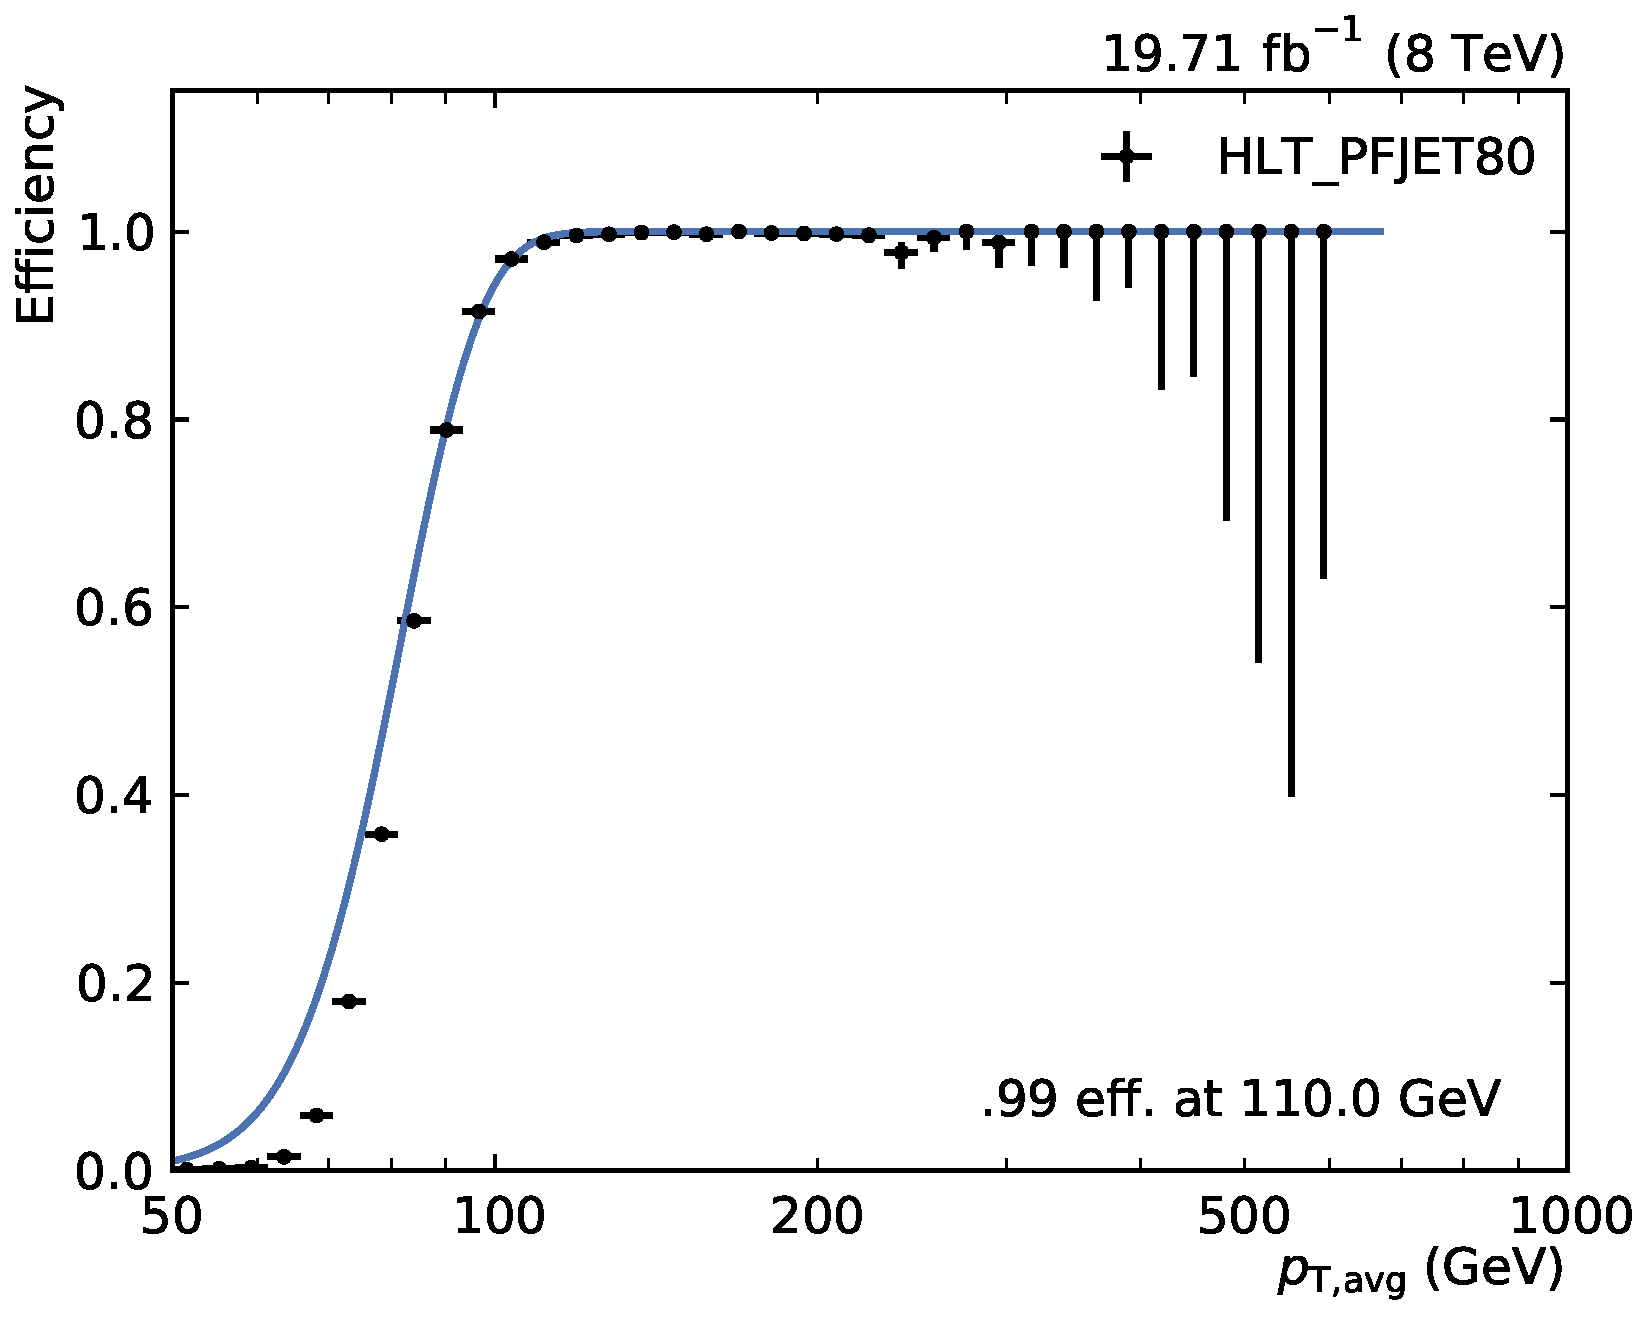
\includegraphics[width=0.49\textwidth]{figures/measurement/trigger_eff_HLT_PFJET80_default.pdf}\hfill
    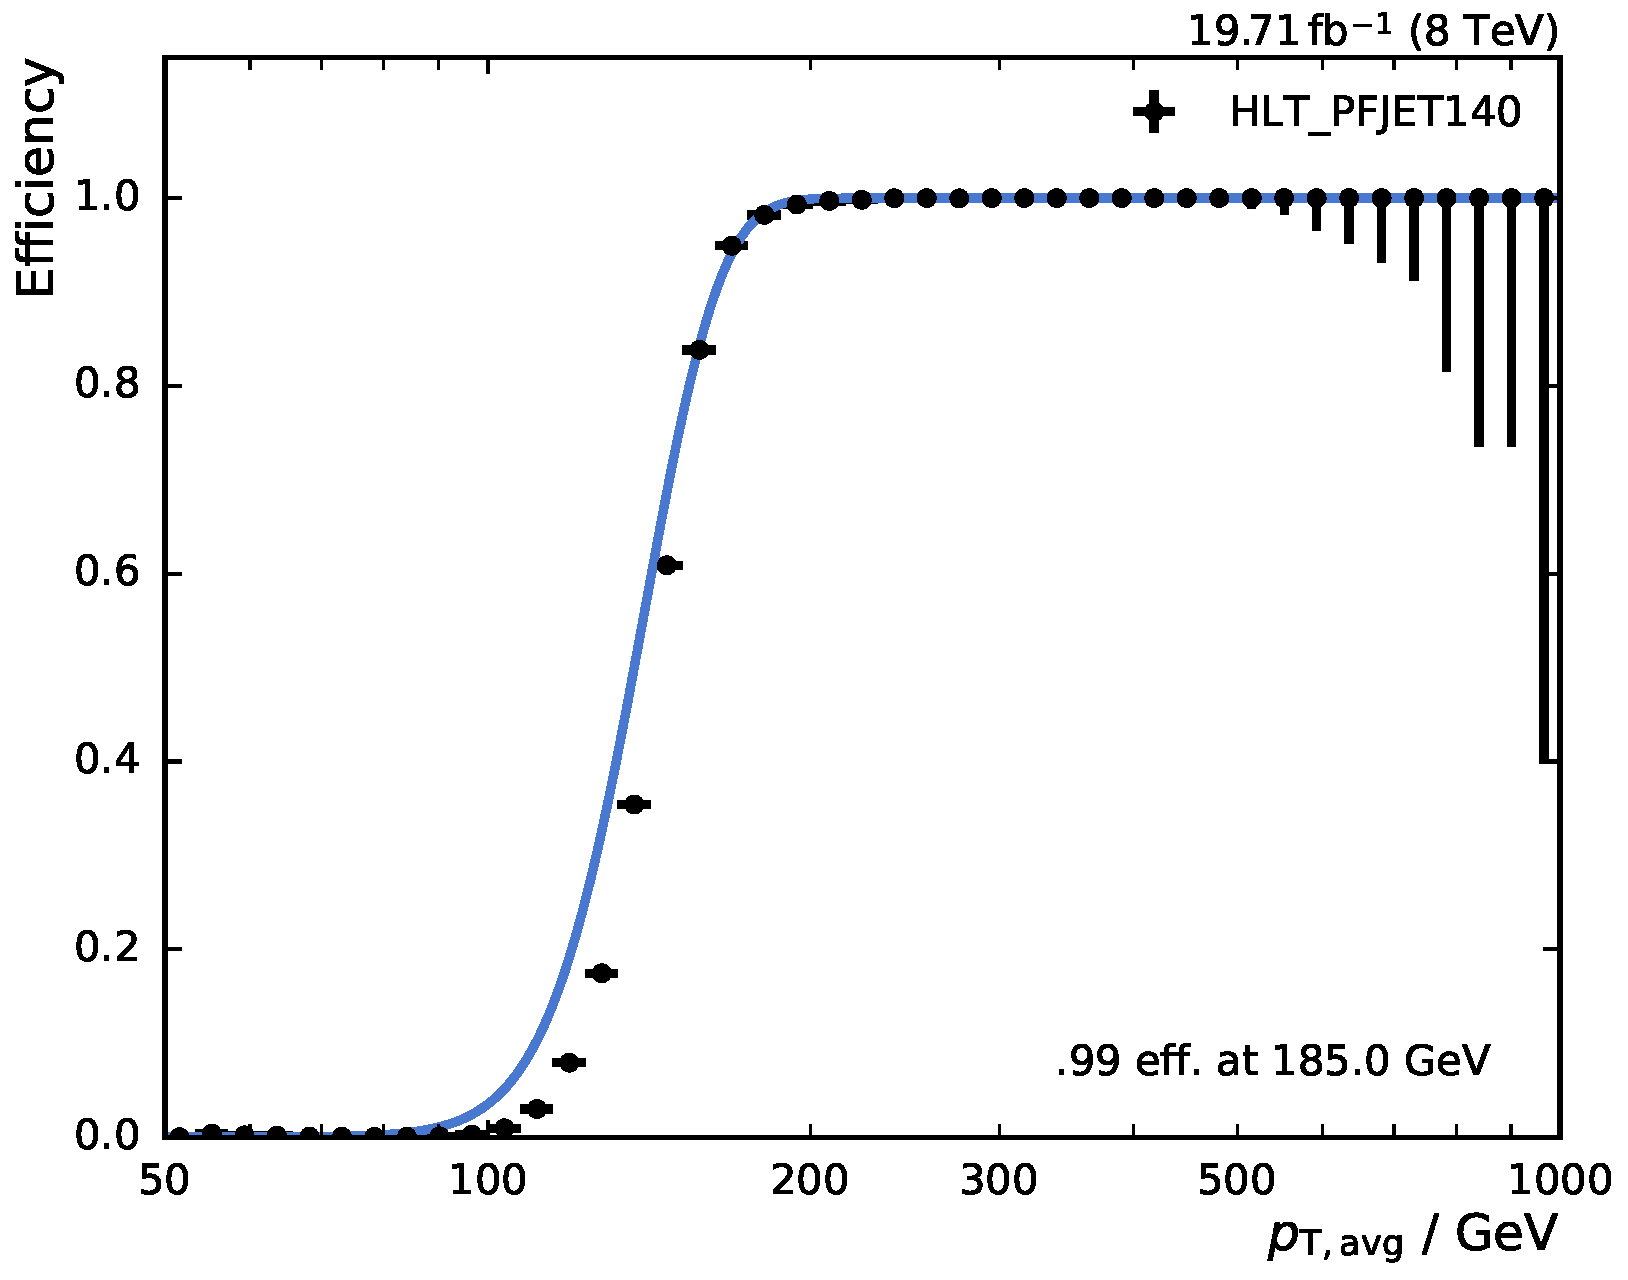
\includegraphics[width=0.49\textwidth]{figures/measurement/trigger_eff_HLT_PFJET140_default.pdf}
    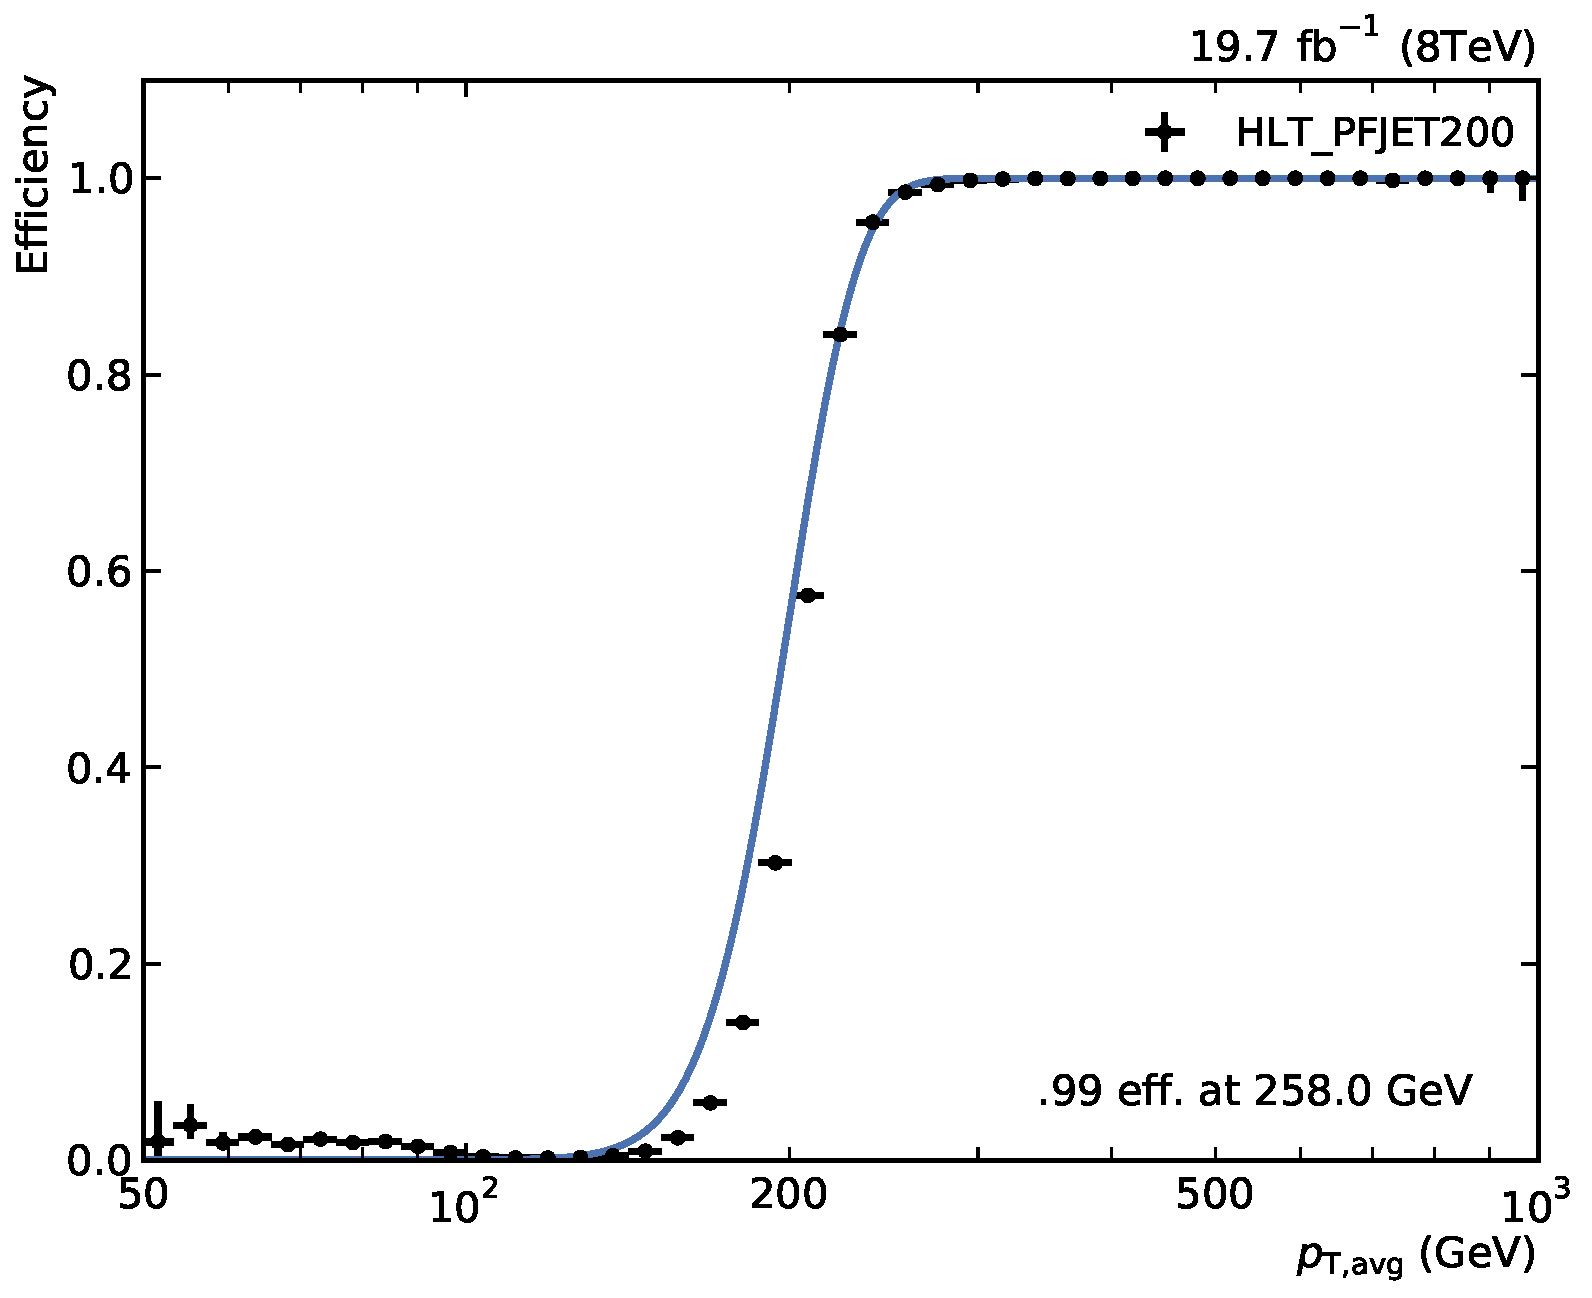
\includegraphics[width=0.49\textwidth]{figures/measurement/trigger_eff_HLT_PFJET200_default.pdf}\hfill
    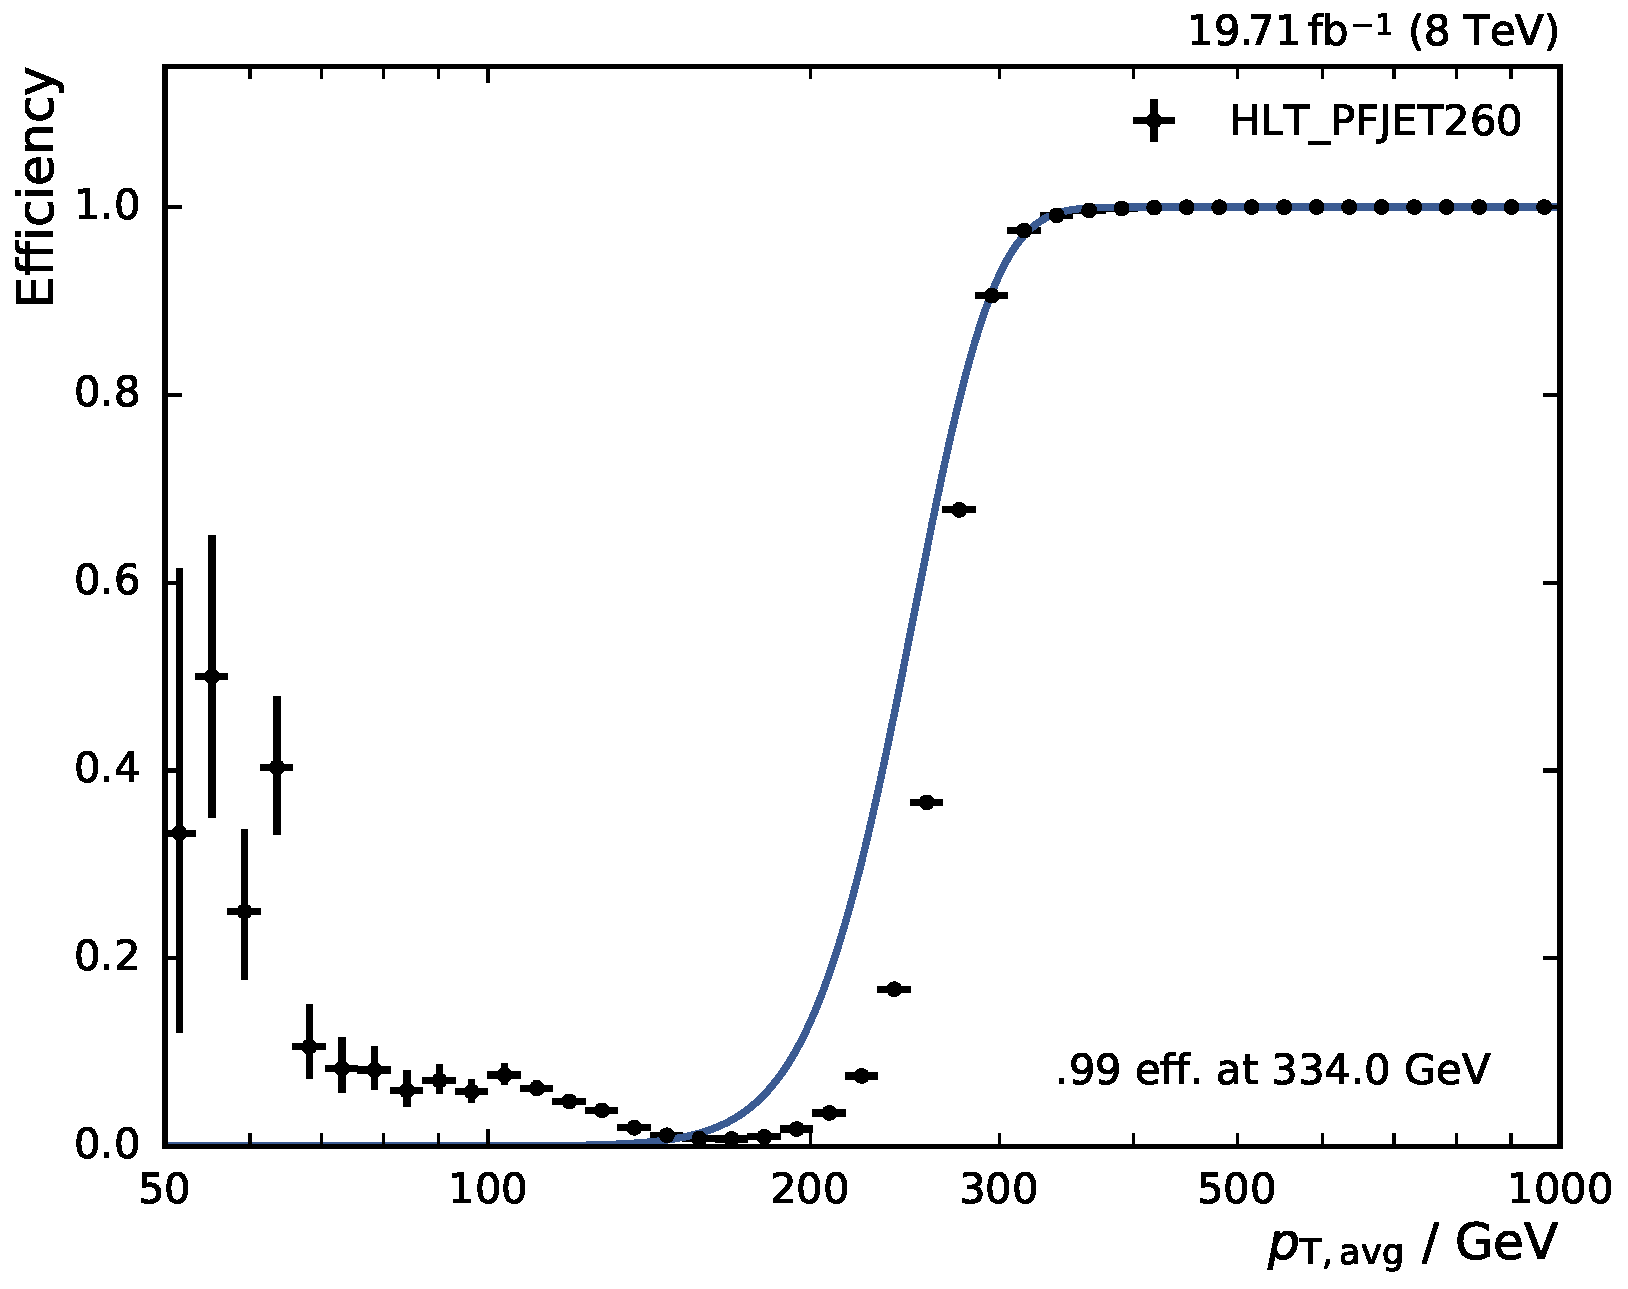
\includegraphics[width=0.49\textwidth]{figures/measurement/trigger_eff_HLT_PFJET260_default.pdf}
    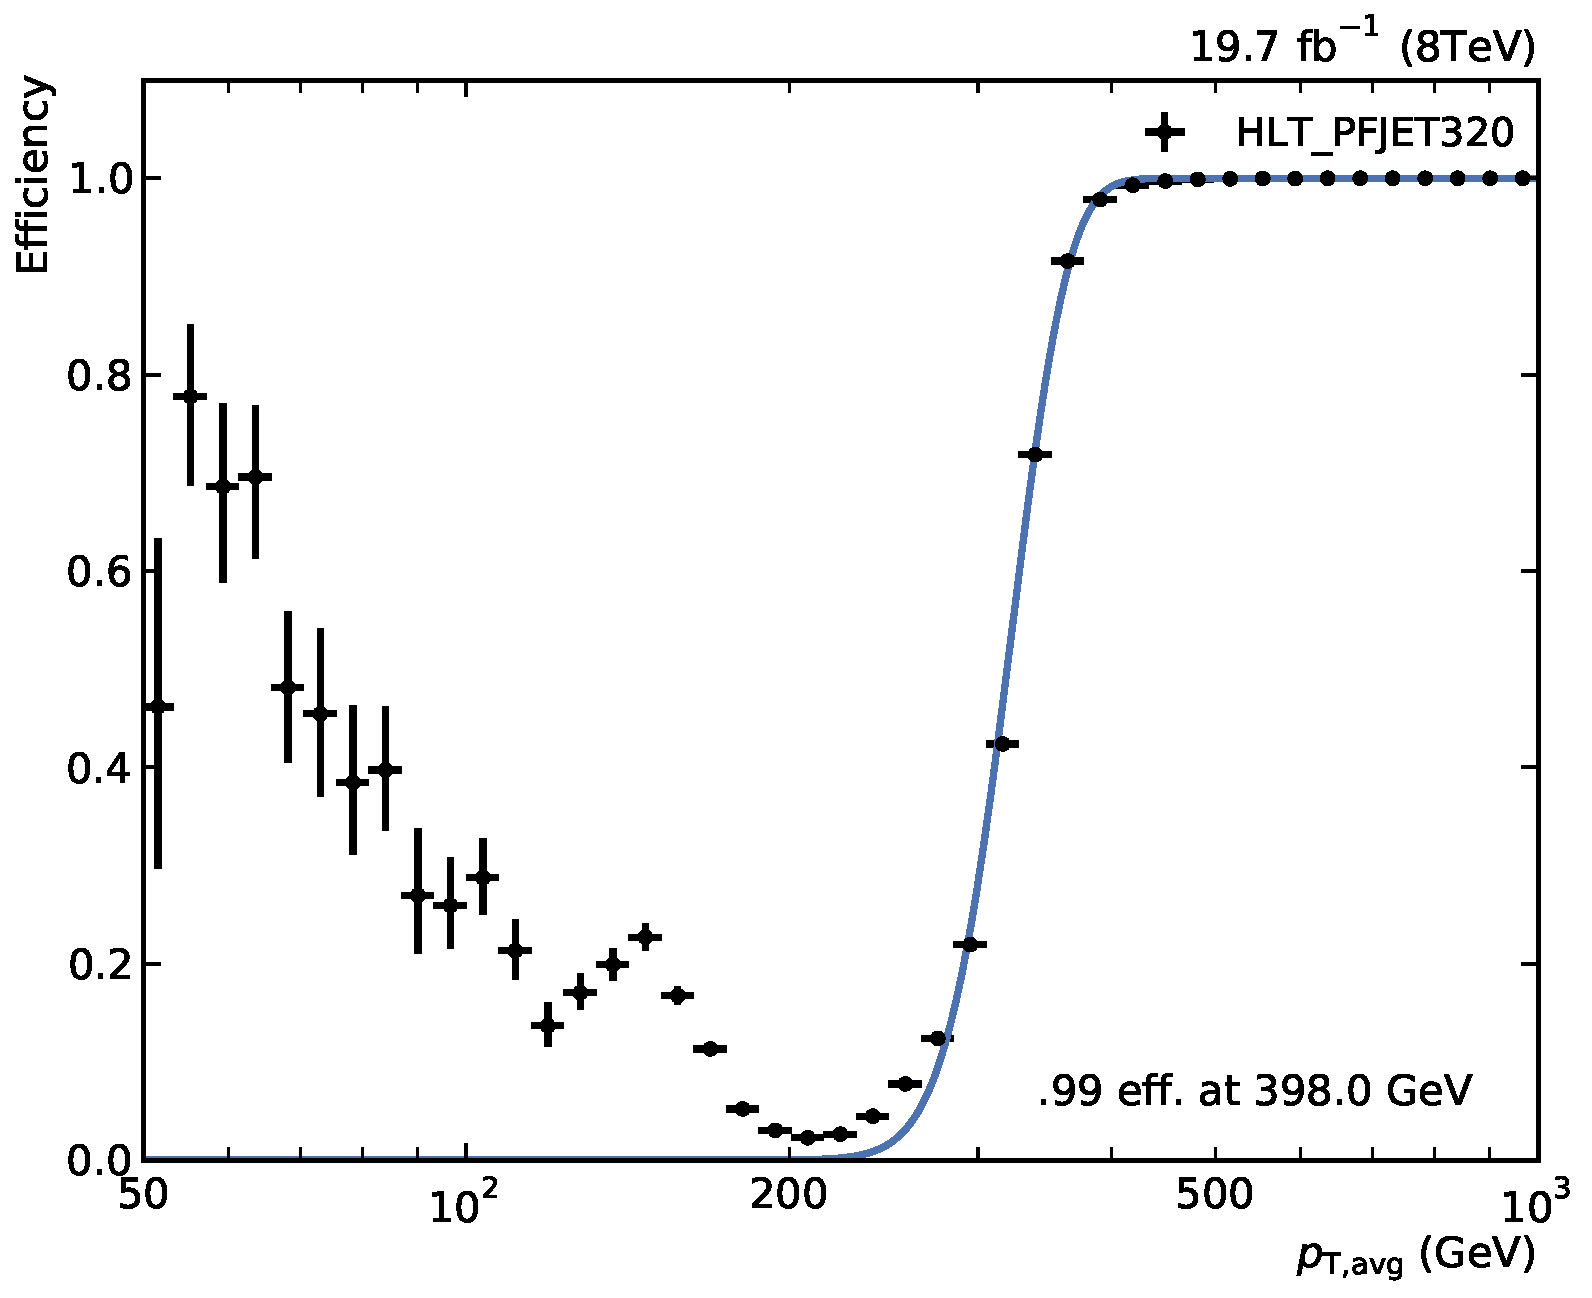
\includegraphics[width=0.49\textwidth]{figures/measurement/trigger_eff_HLT_PFJET320_default.pdf}\hfill
    \caption[Turn-on curves of single jet HLT trigger paths]{Trigger turn-on curves for the single jet trigger
    paths used in the analysis. To determine the 99\% efficiency threshold, the
    trigger turn-on curves are fitted using a sigmoid function taking into account the
    uncertainties using Clopper-Pearson confidence intervals.}
    \label{fig:trigger_eff}
\end{figure}

The jet reconstruction algorithms and the jet energy corrections applied on HLT
level slightly differ from the ones used for the final event reconstruction.
Furthermore, the efficiency of each trigger is not calculated as a function of
jet \pt, which was used in the trigger decision, but versus \ptavg of the two
leading jets as used in this analysis. Therefore, the triggers exhibit a turn-on
behavior, as can been seen in Fig.~\ref{fig:trigger_eff}. Consequently, it is
necessary to determine the threshold above which a trigger becomes fully
efficient. It is defined as the value at which the efficiency exceeds 99\%.

Basically, it is possible to calculate the efficiency of a given trigger by
dividing the number of passing events through the number of events that pass
the next-lower trigger in \pt, because by definition the looser trigger is efficient,
as soon as the higher trigger becomes efficient. This is aggravated through the
different prescales applied to each trigger path. While it is possible to
normalize the yield by the effective luminosity seen by each trigger, this
method is affected by larger statistical fluctuations as the number of events
differs strongly between the two trigger paths.

Therefore, a more challenging but superior method is employed: When the L1
and HLT triggers are processed, the jet four-vectors, on
which the trigger decision is based, are stored. Thus, it is possible to
recalculate the trigger decision by comparing the transverse momentum of the L1
trigger object with the L1 threshold and the \pt of the HLT trigger object with
the HLT threshold~\cite{Stober:2012abc}.

Similarly, the trigger decision of the next higher trigger can be emulated
starting from a lower trigger path. A set of events $S_1 = \left\{E_i | T_A
(E_i)\right\}$ which was accepted  by the lower trigger path $T_A$ is
used to determine the subset $S_2 = \left\{E_i|T_A(E_i) \wedge  T_B(E_i)
\right\}$ which also passes the next higher trigger $T_B$, see
Eq.~\ref{eq:trigger_eff}. The quotient of both event sets is used to determine
the turn-on curve as shown for each trigger path in Fig.~\ref{fig:trigger_eff}. 
The uncertainty on the efficiency is
indicated by error bars which represent Clopper-Pearson confidence intervals.

\begin{equation}
\label{eq:trigger_eff}
    f_{\mathrm{eff}} (x) = \frac{N(\left\{E_i|T_A(E_i) \wedge T_B(E_i), x)\right\}}{N(\left\{ E_i | T_A(E_i)\right\} , x)}
\end{equation}

To determine the point, at which the trigger efficiency is larger than 99\%, the
turn-on distribution is fitted using a sigmoid function that describes the
turn-on behavior of the trigger paths close to the efficiency threshold.

\begin{equation}
\label{eq:trigger_eff_fit}
    f_{\mathrm{fit}} (x) = \frac{1}{2} \left( 1 + \erf \left(\frac{x-\mu}{\sqrt{2}\sigma}\right)\right)
\end{equation}

The thresholds which were finally used in the data analysis deviate slightly
from the ones shown in Fig.~\ref{fig:trigger_eff} as the trigger thresholds
were measured separately in each \ystar and \yboost bin. The most
conservative, thus the highest threshold, is finally chosen. They are reported in
Table~\ref{tab:triggers}.

It is important to mention the HLT triggers which specifically trigger on the
average transverse momentum of the two leading jets and have been implemented
for dijet calibration purposes. At first, they appear to be the obvious choice
for this analysis. However, studies of these triggers revealed, that the
performance is at best comparable to the single jet triggers. Larger prescales
applied to the \ptavg trigger paths result in larger statistical uncertainties.
Therefore, the single jet trigger paths were used in this analysis.

\subsection{Primary Vertex Selection}

The cuts on the primary vertices further reject beam background and off-center bunch
crossings. Each event has to contain at least one primary vertex (PV) which is well
reconstructed within a distance of $|z_\mathrm{PV}| < \SI{24}{\centi \meter}$ to
the nominal interaction point of the detector. Furthermore, the radial distance
$\rho_\mathrm{PV}$ needs to be smaller than $\SI{2}{\centi\meter}$. To
ensure a high quality of the vertex reconstruction, the number of
degrees of freedom in the vertex fit, $n_{\mathrm{dof,PV}}$, needs to be at least
four. Thus, at least four tracks must be present in order to
perform a valid vertex fit.

\subsection{Missing Transverse Energy Cut}

If all particles could be identified and perfectly measured, the transverse
momentum of all particles would sum up to zero. The imbalance in the transverse
momentum of all visible particles, which can be measured in the detector, is
called the missing transverse momentum (MET). Neutrinos, for example, leave the
detector undetected and contribute to the MET. MET is an important ingredient
in many measurements involving W bosons, top quarks or searches for physics
beyond the Standard Model which involve undetectable particles. 

\begin{figure}[htbp]
    \centering
    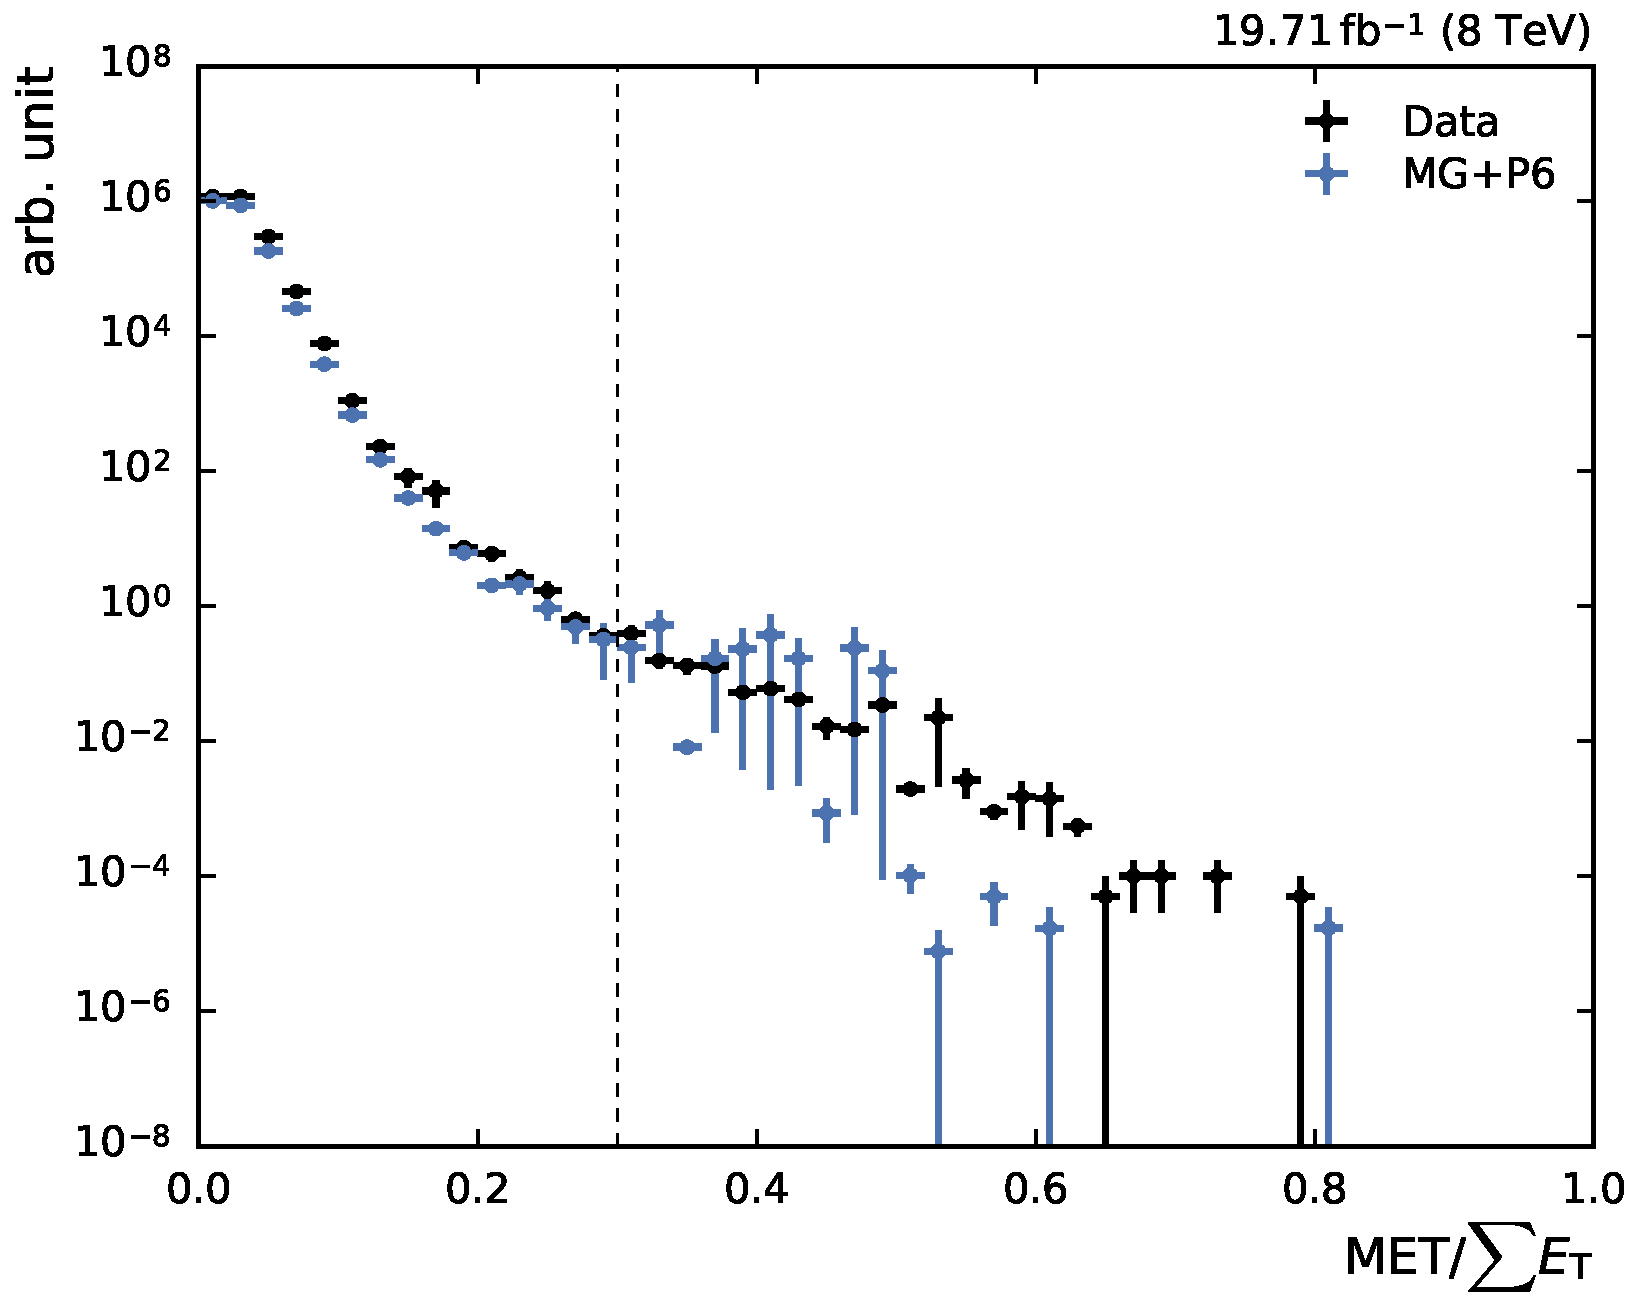
\includegraphics[width=0.7\textwidth]{figures/measurement/metoversumet.pdf}
    \caption[Missing transverse energy distribution]{Missing transverse energy
    fraction of the total transverse energy per event in data and simulated
    events. To remove background and noise, events with a fraction exceeding a
    certain threshold, here indicated by the dashed line, are rejected.}
    \label{fig:mc:met_fraction}
\end{figure}

However, a large fraction of MET in an event is not always caused by interesting
physics processes. Very often, the reason can be found in detector noise, cosmic
rays or beam-halo particles. Therefore, a sequence of algorithms developed by
the MET working group at CMS~\cite{jetmet:metfilters} is employed, which
identifies and rejects these events. Moreover, a cut removing events in which
the missing transverse energy fraction \met constitutes a large fraction of the
total transverse energy $\sum_i E_{\mathrm{T},i}$ is applied, see
Fig.~\ref{fig:mc:met_fraction},

\begin{equation}
    \frac{\met}{\sum_i E_{\mathrm{T},i}} < 0.3.
\end{equation}

\subsection{Jet Identification}

The jet identification criteria (jet ID) reject noise and noise-enhanced jets
while all real jets are kept. The jet ID is not applied per event, but each jet
is accepted or removed from the list of valid jets. The algorithm works on
reconstructed jets using information of the clustered particle candidates.
Following the official recommendations of the \textsc{JetMET}
group~\cite{jetmet:jetid}, the so-called loose jet ID is used. All jets passing the jet ID
are then further processed in the analysis chain. 

The properties of the reconstructed jets and their respective cuts are listed in
Table~\ref{tab:jetid}. The cut on the fraction of neutral hadrons and photons
removes HCAL noise and ECAL noise, respectively. Muons that are falsely
identified and clustered as jets are removed by the muon fraction criterion.
Based on information of the tracker, additional selection cuts are enforced in
the region $|\eta| < 2.4$. Jets clustered from misidentified electrons are removed by the
charged electromagnetic fraction cut. Furthermore, the fraction of charged hadrons in the
jet must be larger than zero. This cut is important since the CHS algorithm
removes charged particles from pileup vertices. Consequently, jets without any
charged hadrons are very likely to be pileup jets. The
Figs.~\ref{fig:jet_constituents_fractions} and~\ref{fig:jet_constituents_counts}
show the distributions of the jet constituents observed in data and simulated
events.

\begin{figure}[htbp]
    \centering
    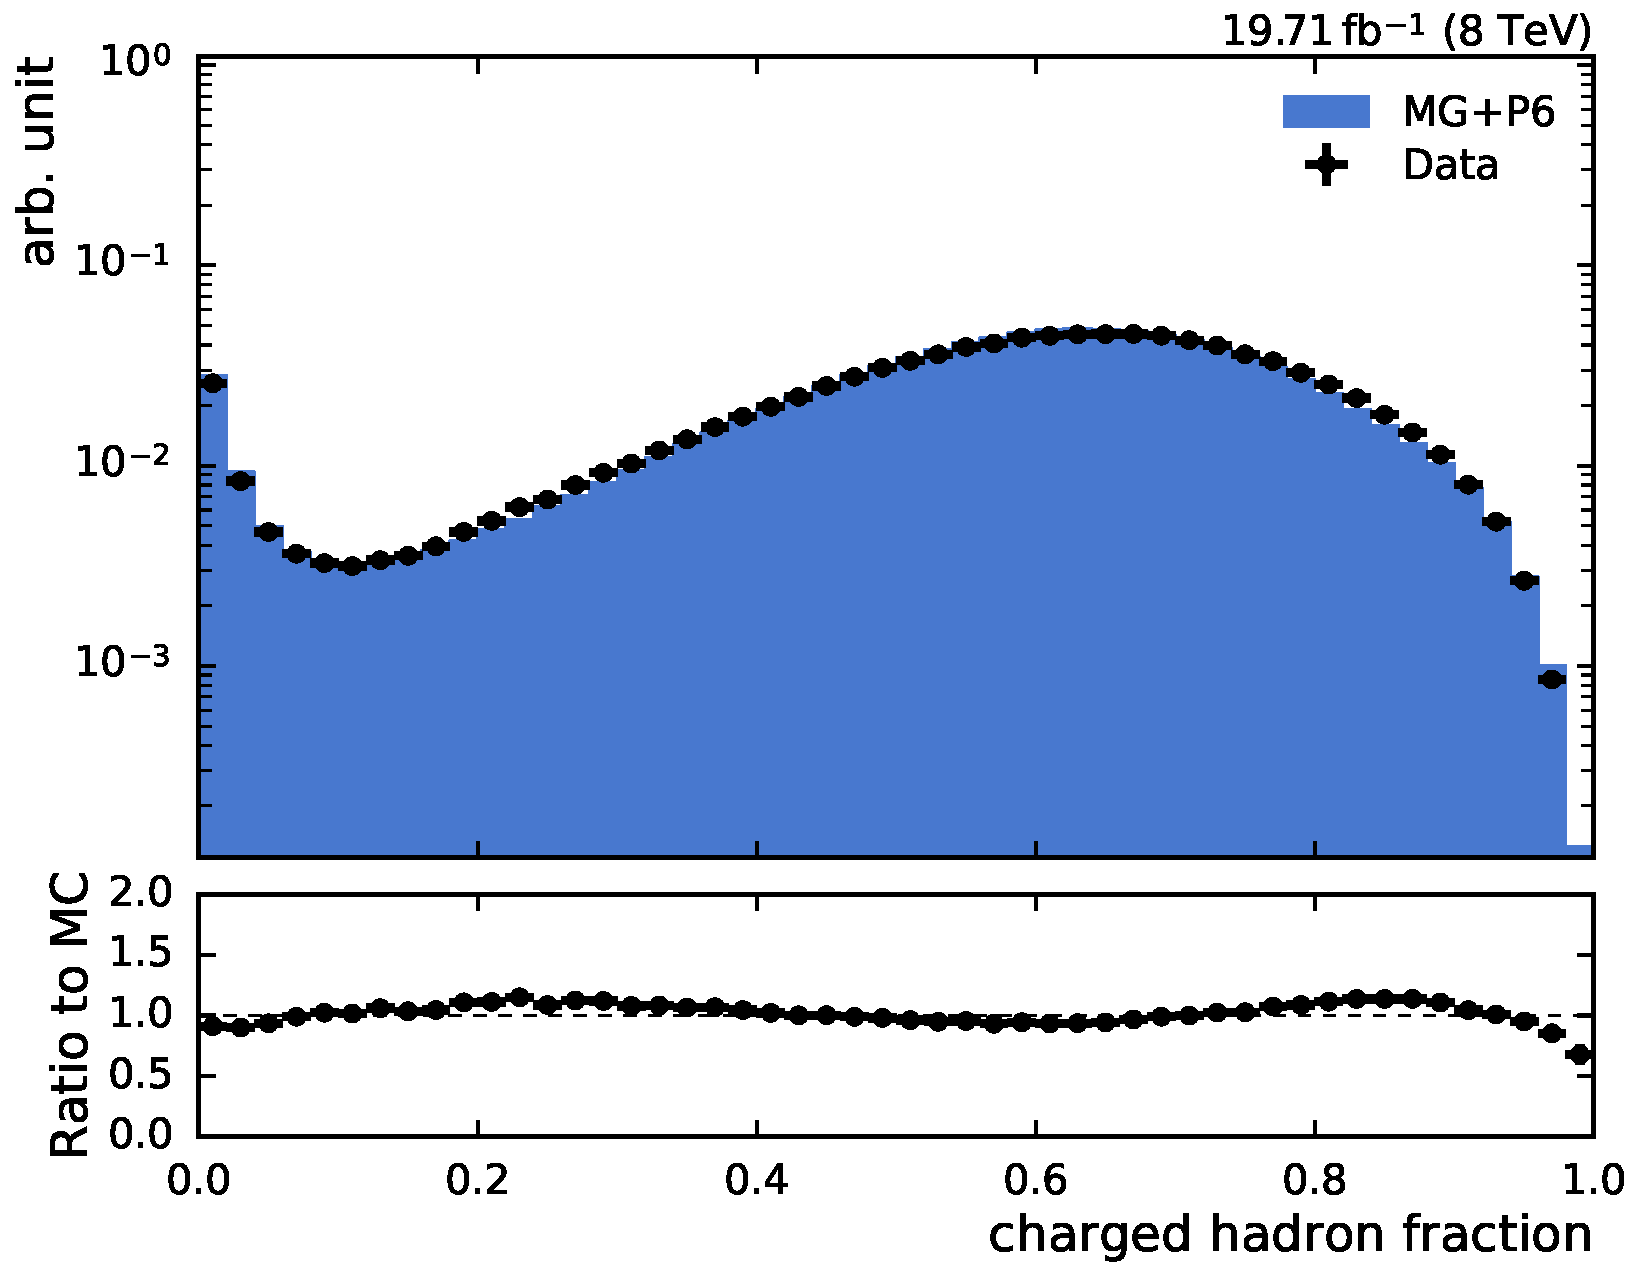
\includegraphics[width=0.49\textwidth]{figures/measurement/jet_constituent_chargedHadronFraction.pdf}\hfill
    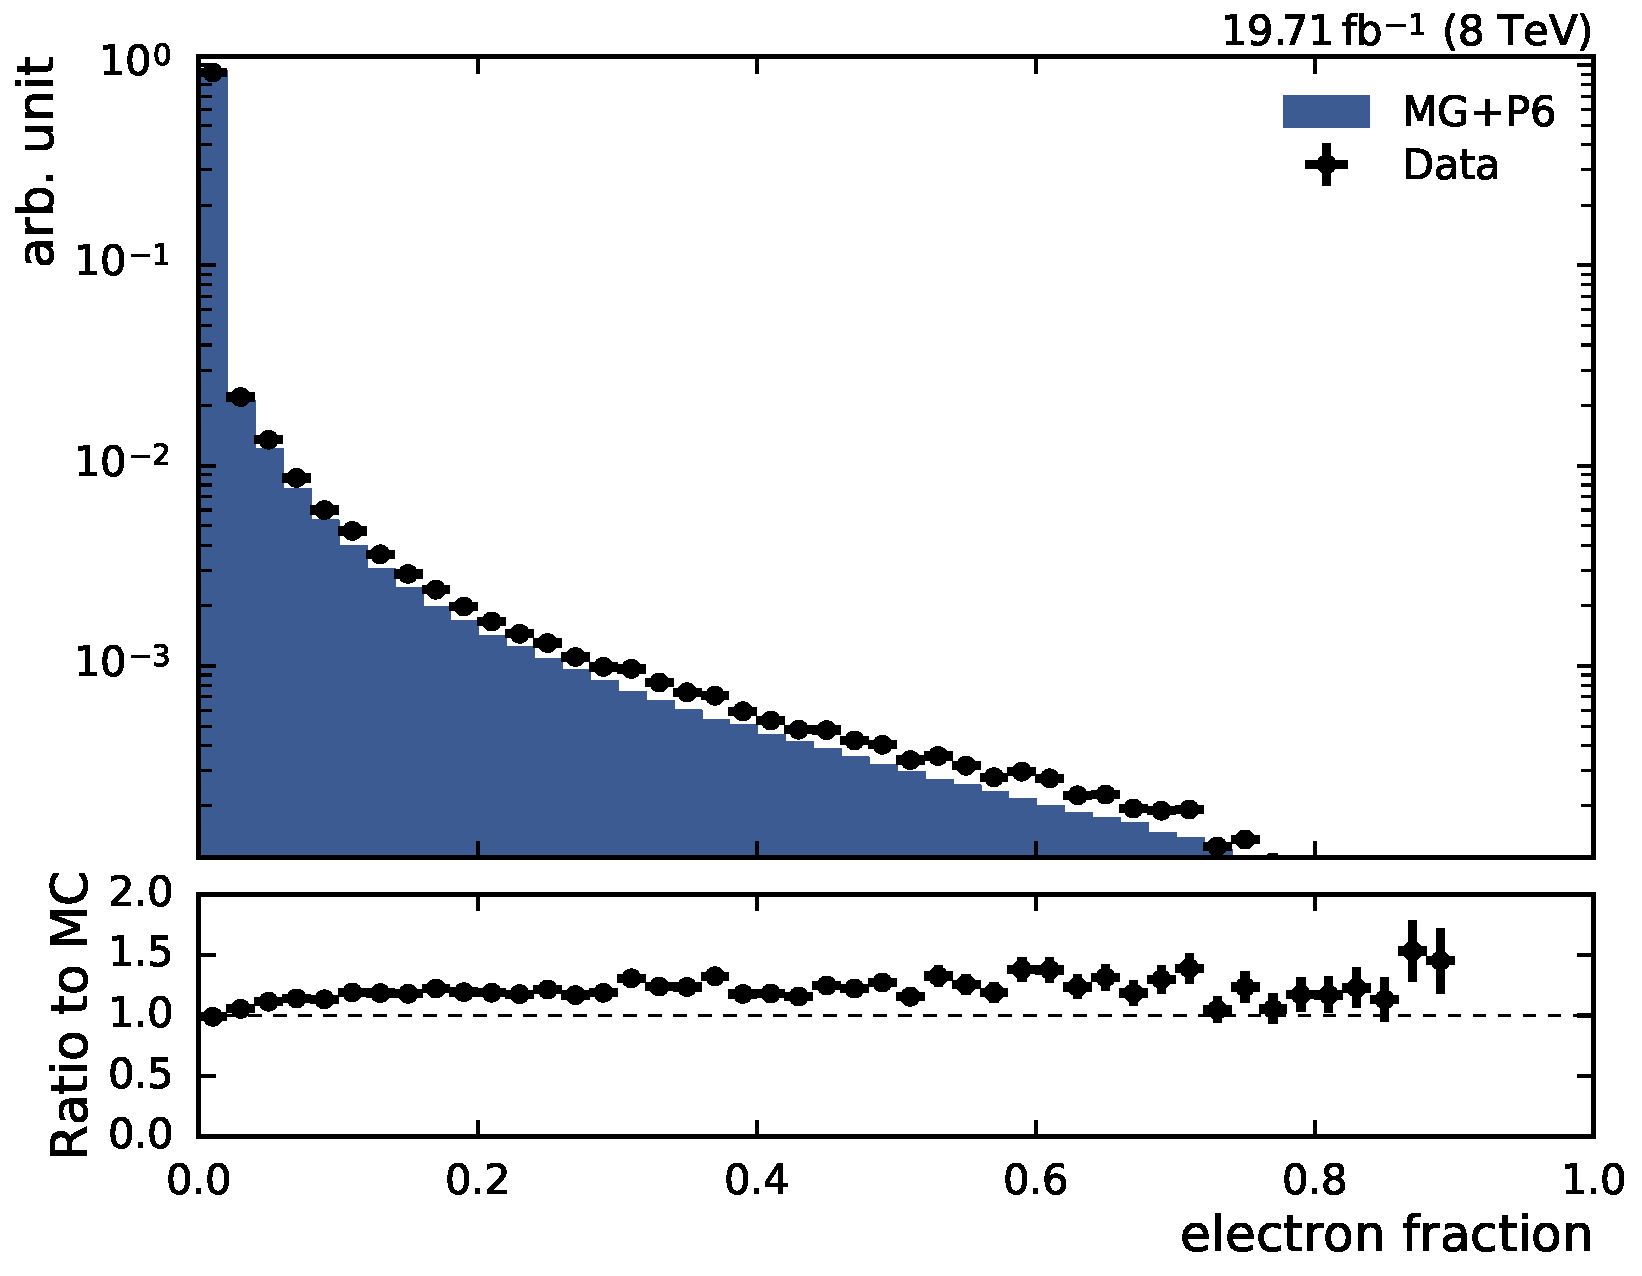
\includegraphics[width=0.49\textwidth]{figures/measurement/jet_constituent_electronFraction.pdf}
    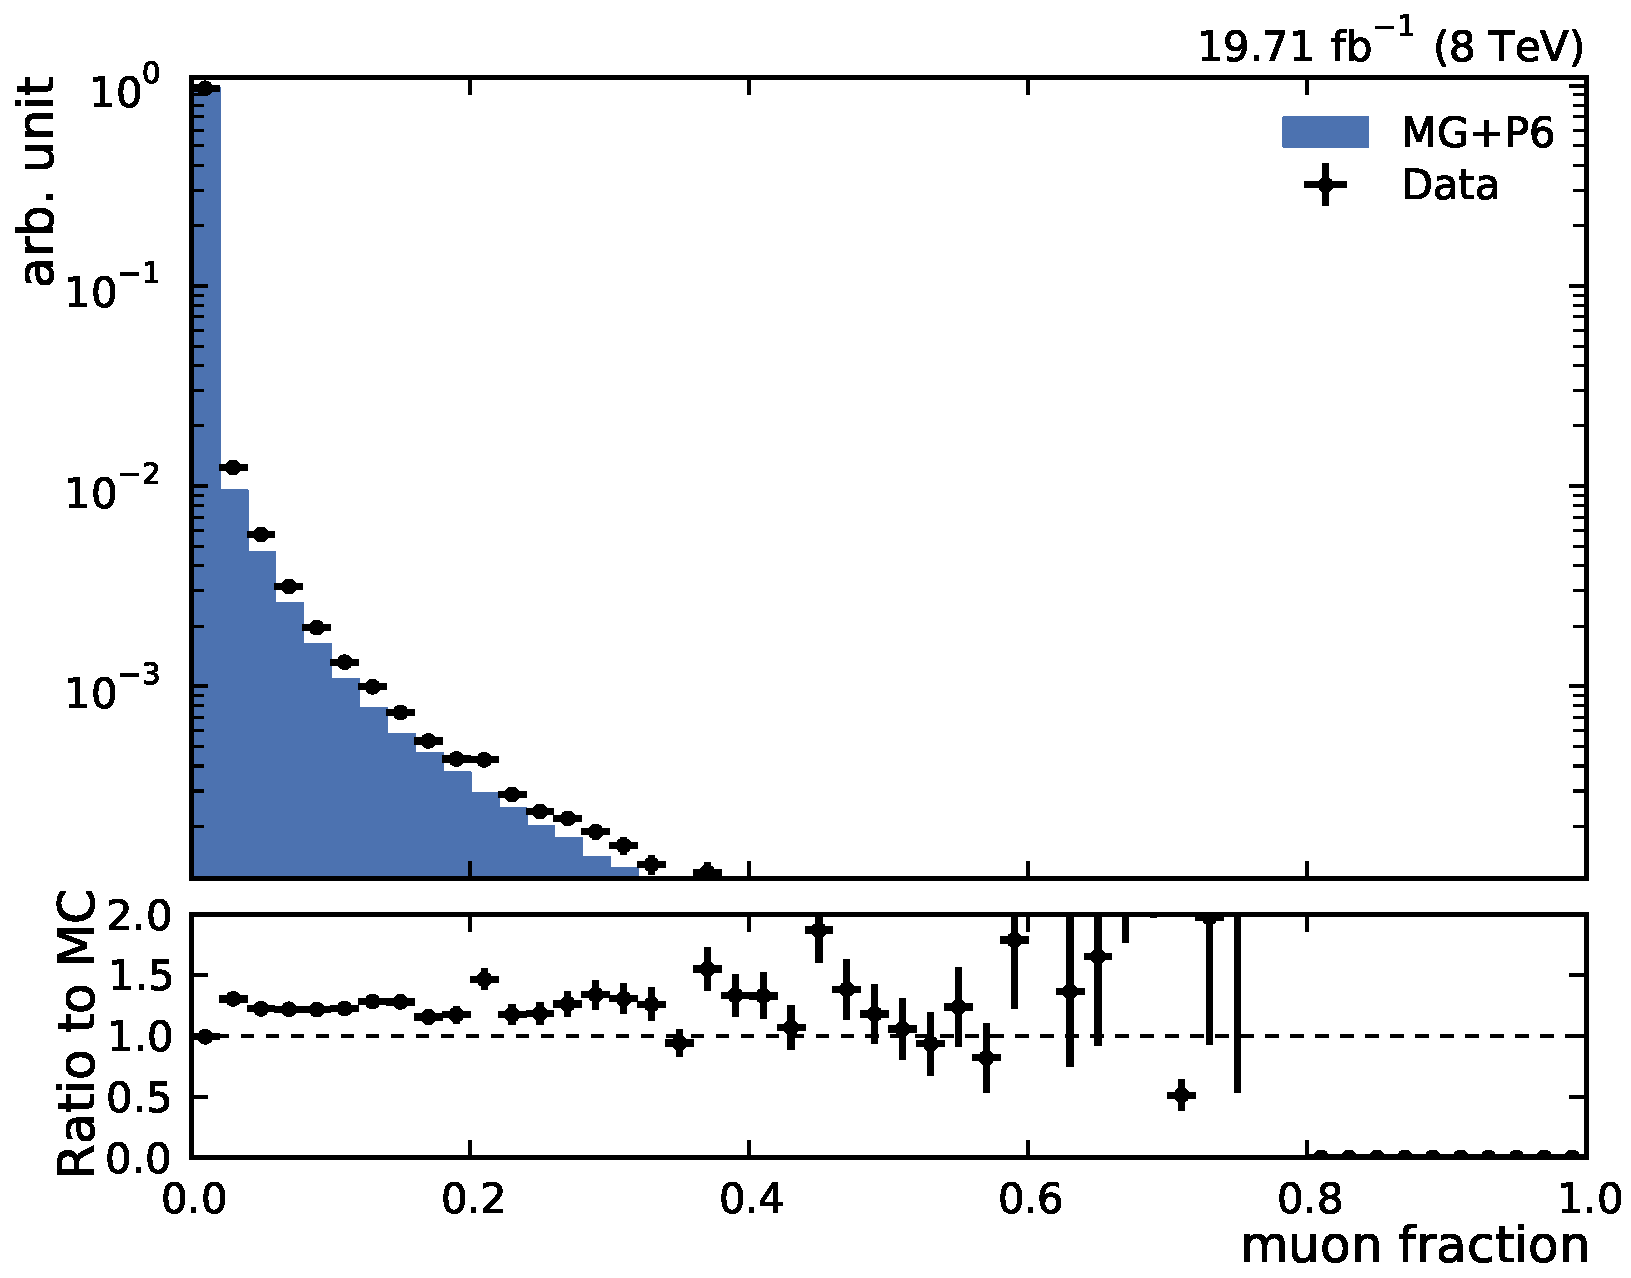
\includegraphics[width=0.49\textwidth]{figures/measurement/jet_constituent_muonFraction.pdf}\hfill
    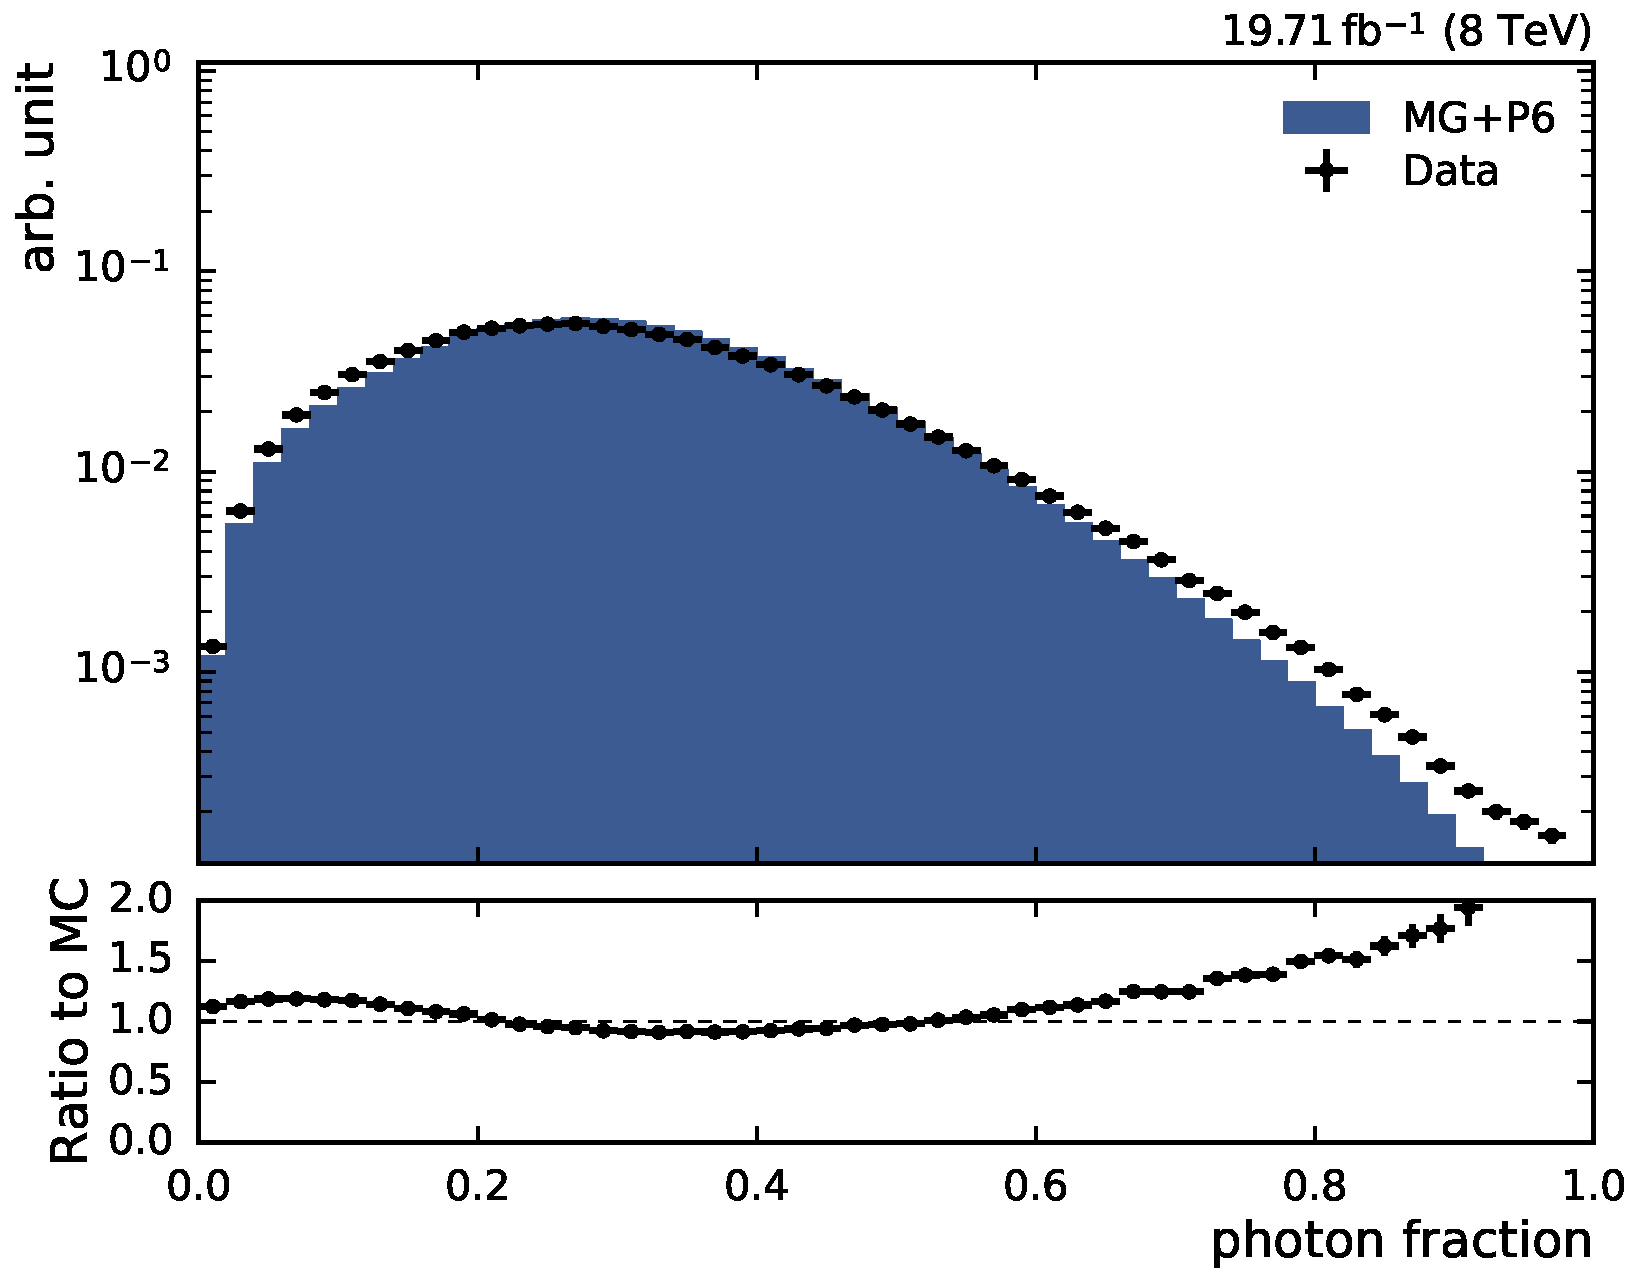
\includegraphics[width=0.49\textwidth]{figures/measurement/jet_constituent_neutralEMFraction.pdf}
    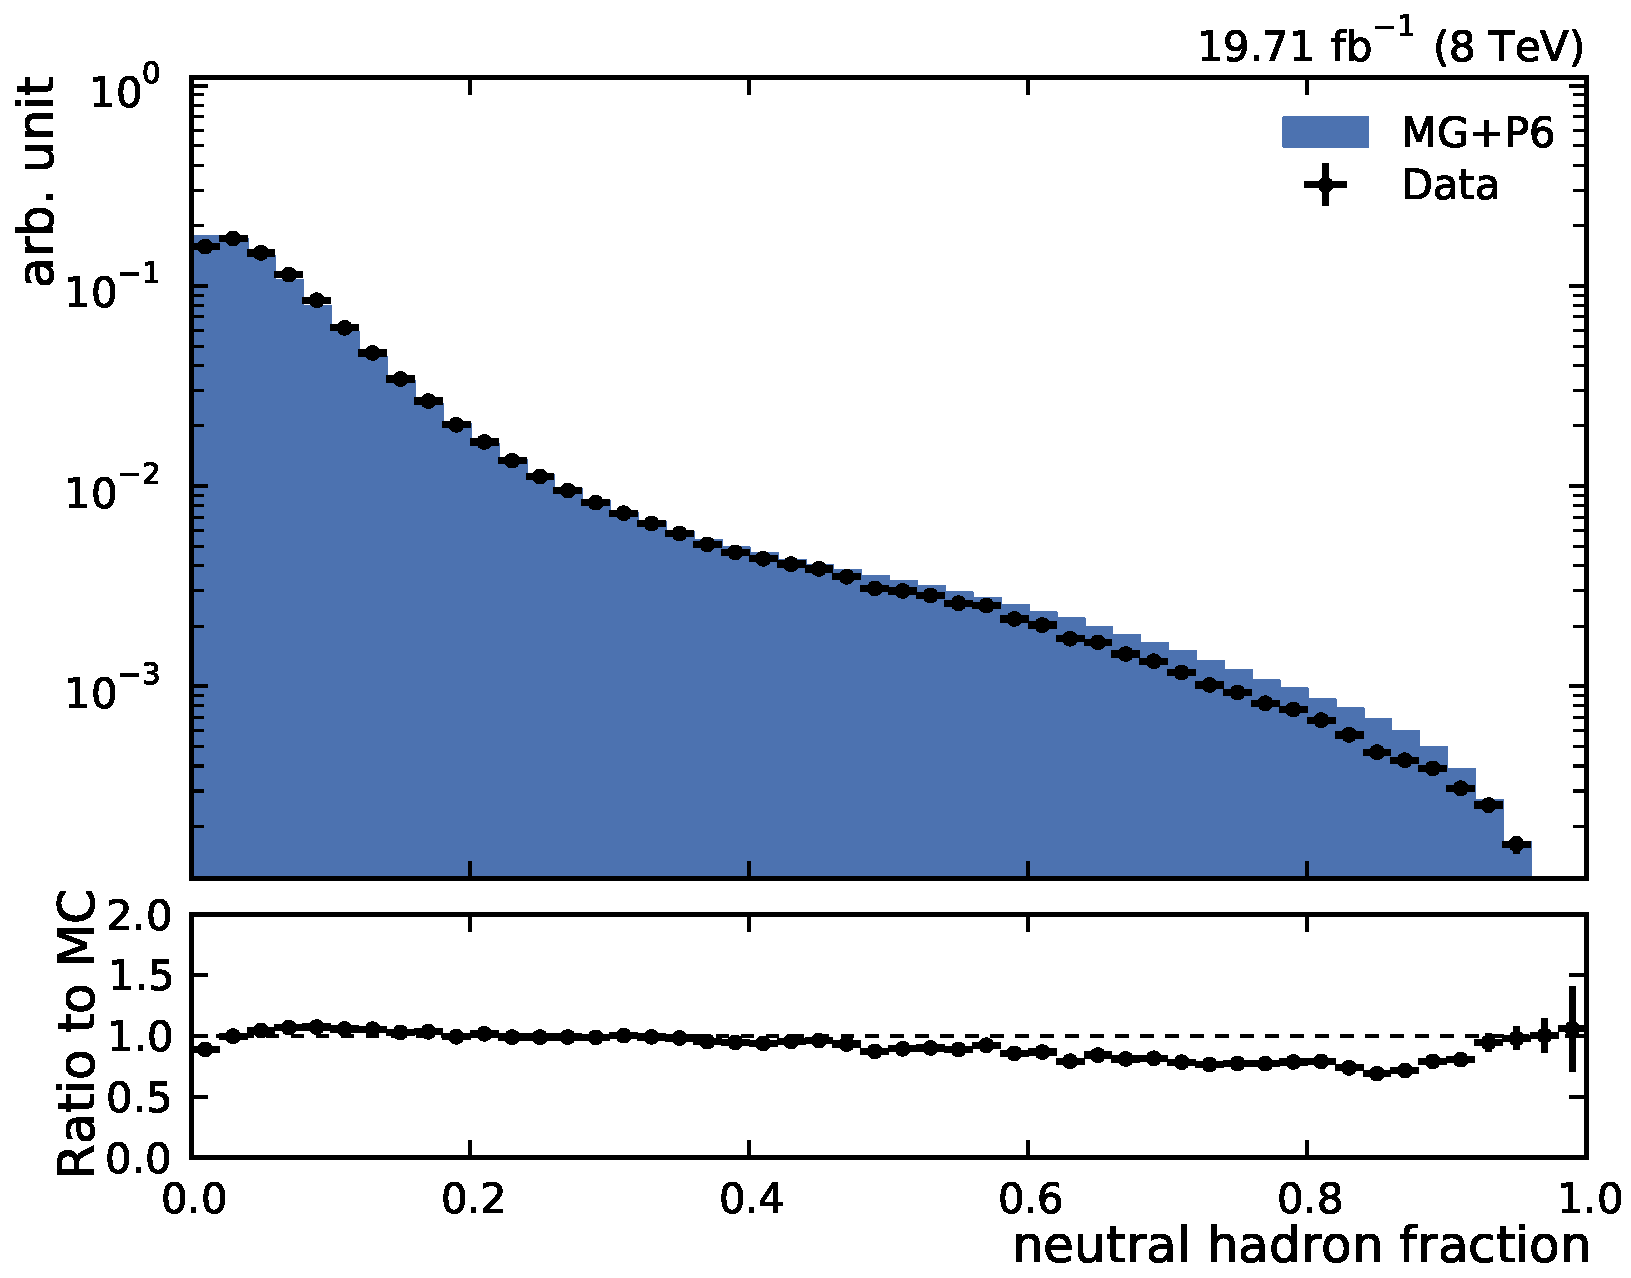
\includegraphics[width=0.49\textwidth]{figures/measurement/jet_constituent_neutralHadronFraction.pdf}
    \caption[PF candidate fractions in jets]{The fractions of jet constituents as
            observed in data and simulated events for different types of PF candidates.
            Data and simulation are normalized to the same number of events. The
            distributions are shown after the application of the jet ID.}
    \label{fig:jet_constituents_fractions}
\end{figure}

\begin{figure}[htbp]
    \centering
    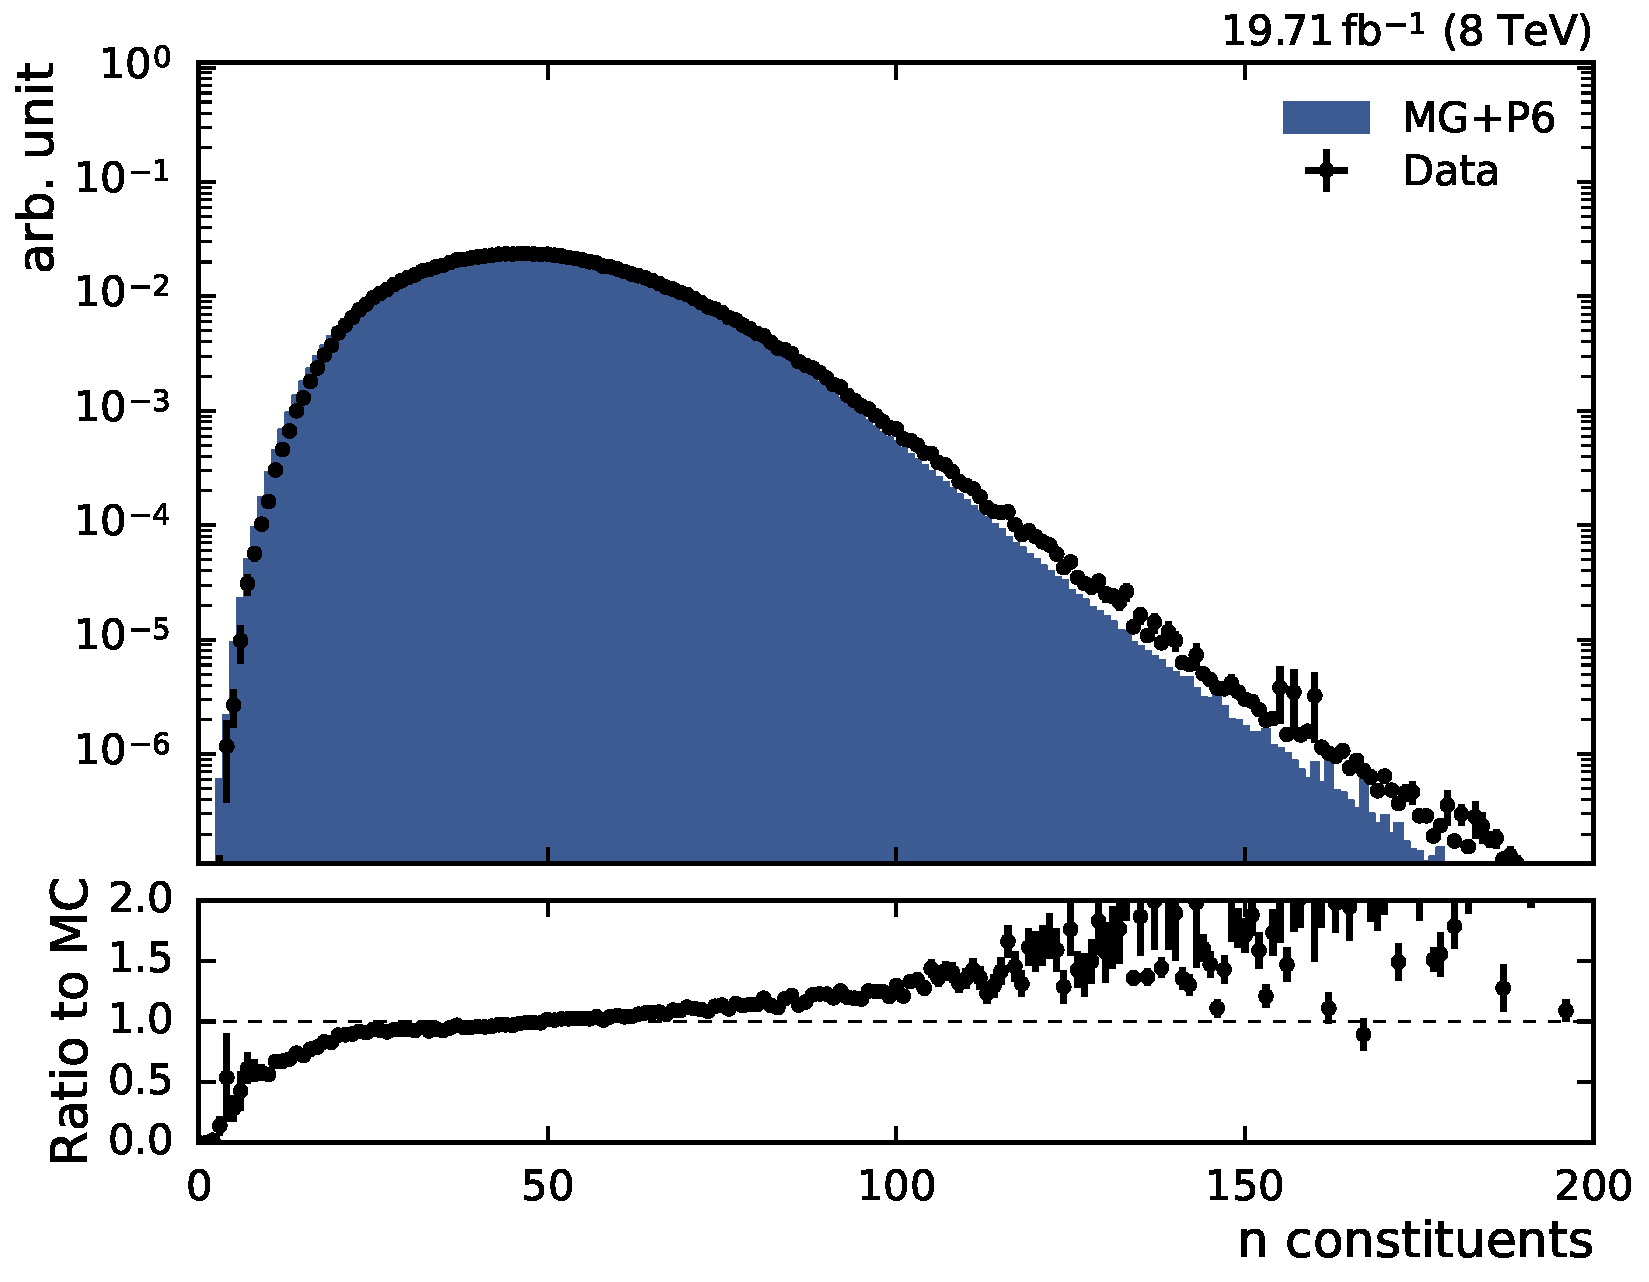
\includegraphics[width=0.49\textwidth]{figures/measurement/jet_constituent_nConstituents.pdf}\hfill
    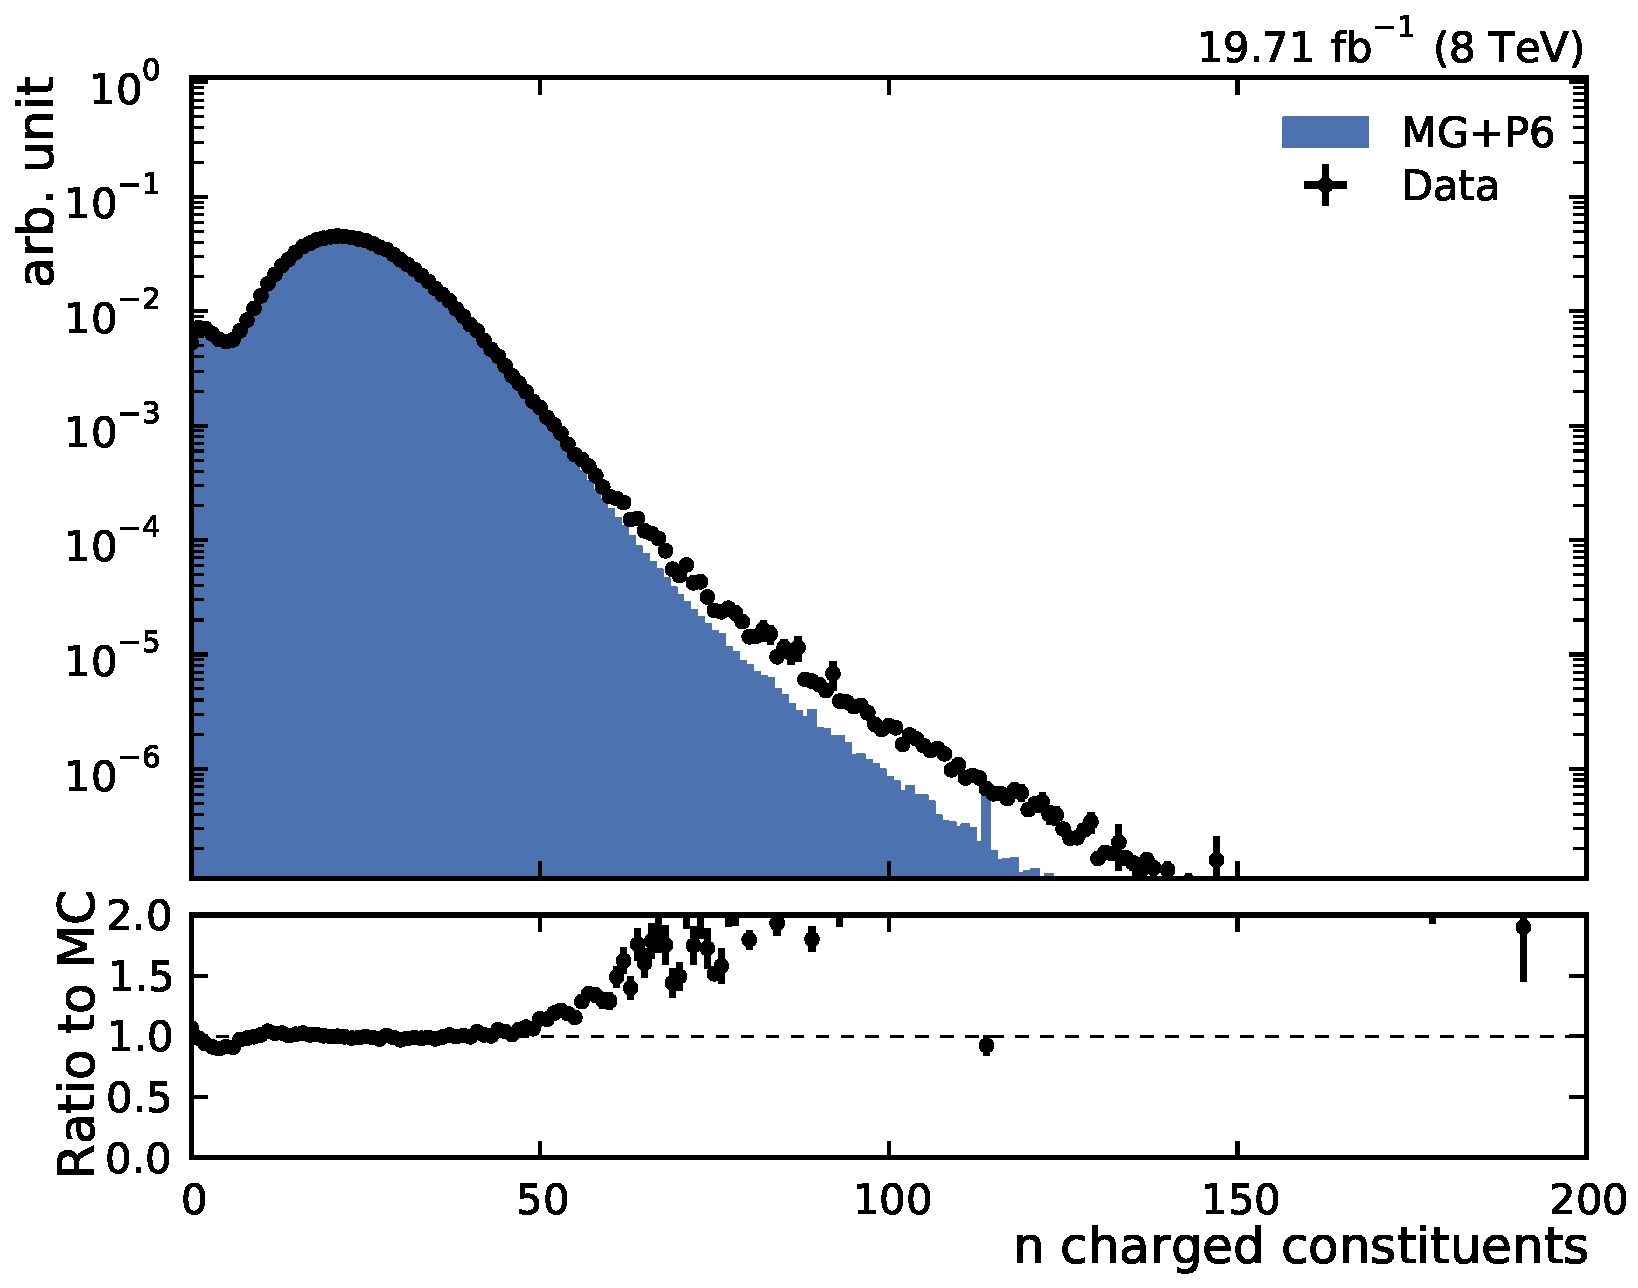
\includegraphics[width=0.49\textwidth]{figures/measurement/jet_constituent_nCharged.pdf}
    \caption[Number of particle candidates in jets]{Number of PF candidates
             clustered into a jet in data and simulated events. Data and simulation are
             normalized to the same number of events.}
    \label{fig:jet_constituents_counts}
\end{figure}

While studying the loose and tight jet criteria, it was found that the tight jet
ID removes a non-negligible fraction of jets in the forward region ($|y| > 2.4$) of the
phase space considered in this analysis. Therefore, the loose jet ID is favored
and applied in this thesis which is also the official recommendation of the
\textsc{JetMET} group.

\begin{table}[htbp]
    \centering
    \caption[Jet ID criteria]{The jet ID removes noise and fake jets based on
        the properties of the reconstructed jets and the clustered particle
        candidates. All selection cuts which are recommended by the
        \textsc{JetMET} group are applied~\cite{jetmet:jetid}. The loose jet ID is
        used in this analysis as the tight ID removes a non-negligible fraction
        of signal events, particularly in the forward region without tracker
        coverage.}
    \label{tab:jetid}
    \begin{tabular}{llll}
    \toprule
                                 & \textbf{Property}       & \textbf{Loose ID} & \textbf{Tight ID}\\\cmidrule(lr){2-4}
                                 \textbf{Whole $\bm{\eta}$ region} &                         &                   & \\\cmidrule(lr){1-1}
                                 & neutral hadron fraction & $< 0.99$          & $< 0.90$\\
                                 & neutral EM fraction     & $< 0.99$          & $< 0.90$\\
                                 & number of constituents  & $> 1$             & $> 1$\\
                                 & muon fraction           & $< 0.80$           & $< 0.80$\\
                                 \textbf{only $\bm{|\eta| < 2.4}$} &                         &                   & \\\cmidrule(lr){1-1}
                                 & charged hadron fraction & $> 0$             & $> 0$\\
                                 & charged multiplicity    & $> 0$             & $> 0$\\
                                 & charged EM fraction     & $< 0.99$          & $< 0.90$\\
    \bottomrule
    \end{tabular}
\end{table}


\subsection{Jet ID Efficiency}

The applied jet ID ensures a high purity of real jet events. The efficiency of
the jet ID in the investigated phase space is studied using a
tag-and-probe technique. Dijet events, in which the leading two jets are well
balanced in $\phi$, are selected using
%
\begin{equation*}
    | \Delta\phi - \pi | < 0.3,
\end{equation*}
%
where $\Delta\phi$ is the azimuthal separation between the two leading jets. One
of the dijets is chosen as tag jet and has to fulfill the loose jet ID. For the
other jet it is examined, whether it also passes the jet ID. The quotient of events in
which the probe jet also passes the criteria versus the total number of dijet
events yields the efficiency. Fig.~\ref{fig:jetid_eff} shows the
efficiency as a function of \ptavg of the dijet system for all \ystar and
\yboost bins. As advertized by the \textsc{JetMET} group, the efficiency is
larger than \SI{99}{\percent} in all phase space regions.

\begin{figure}[htbp]
    \centering
    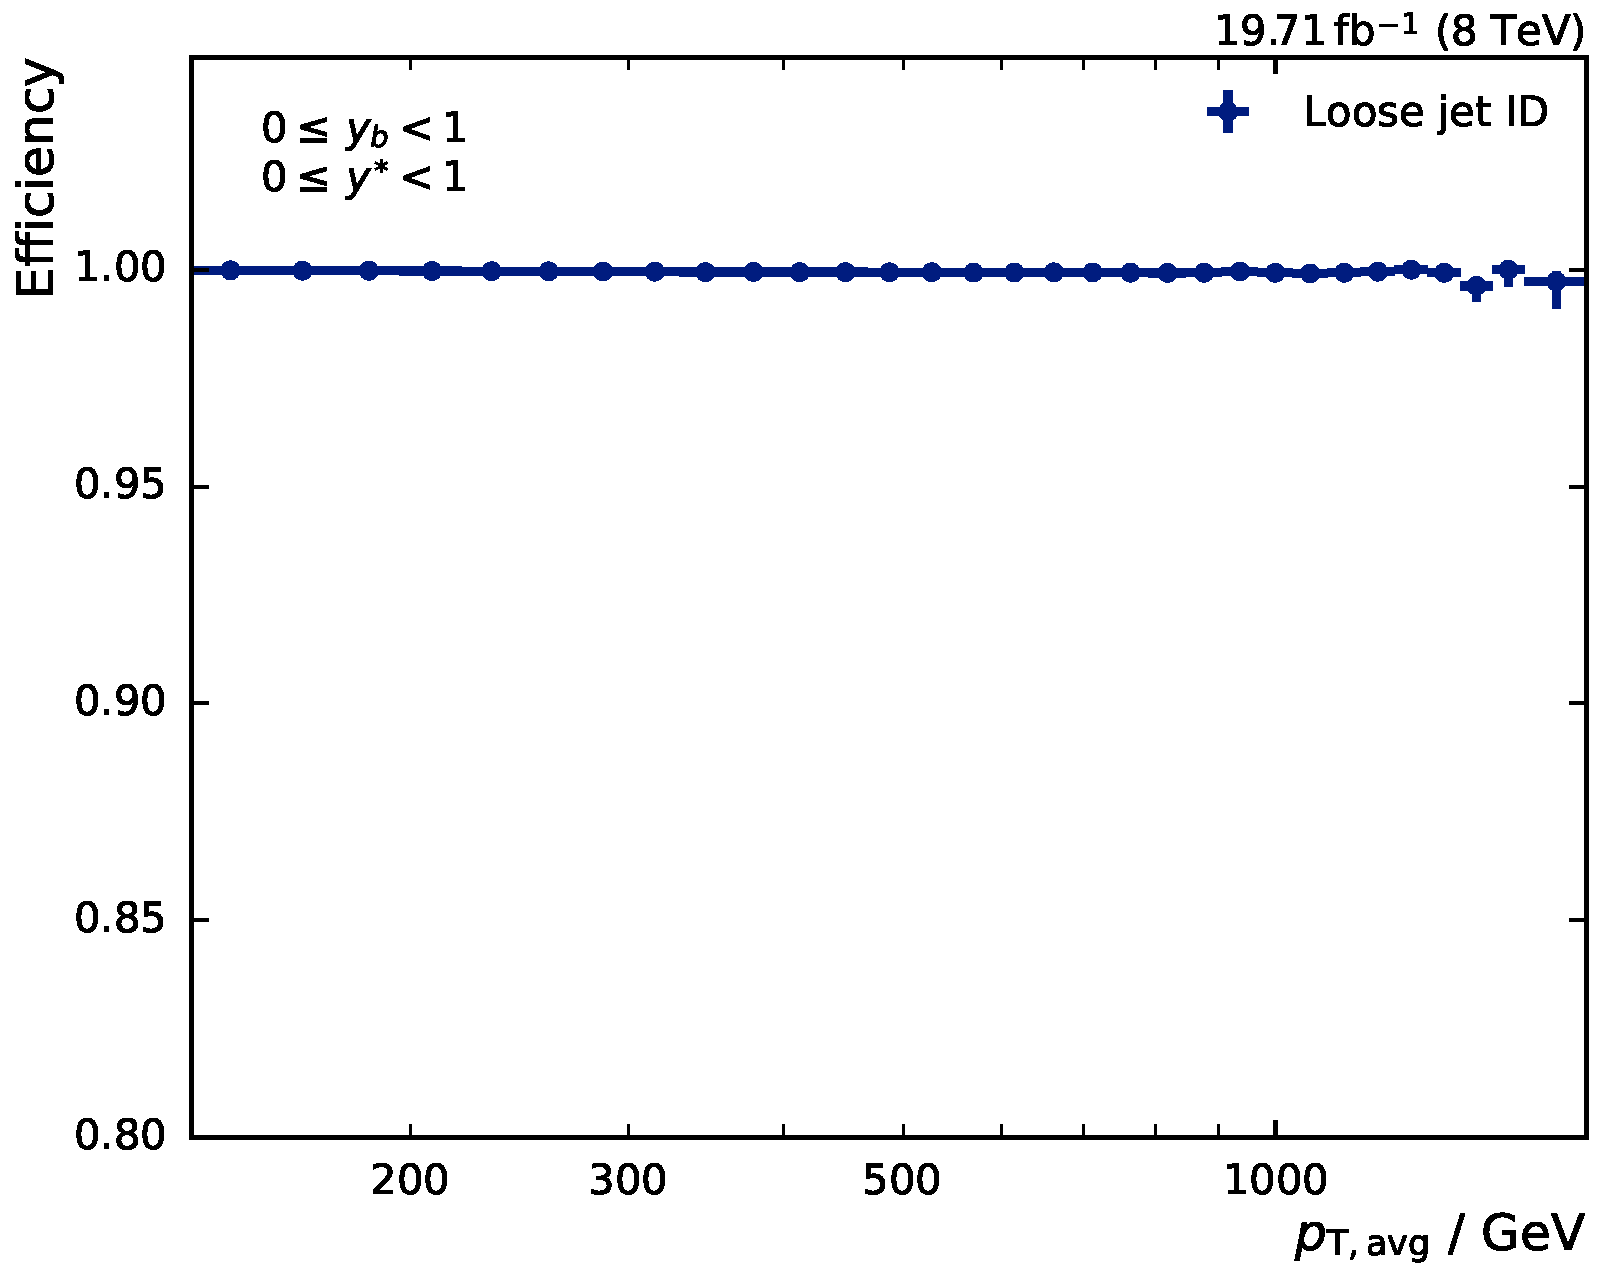
\includegraphics[width=0.49\textwidth]{figures/measurement/jetideff_yb0ys0.pdf}\hfill
    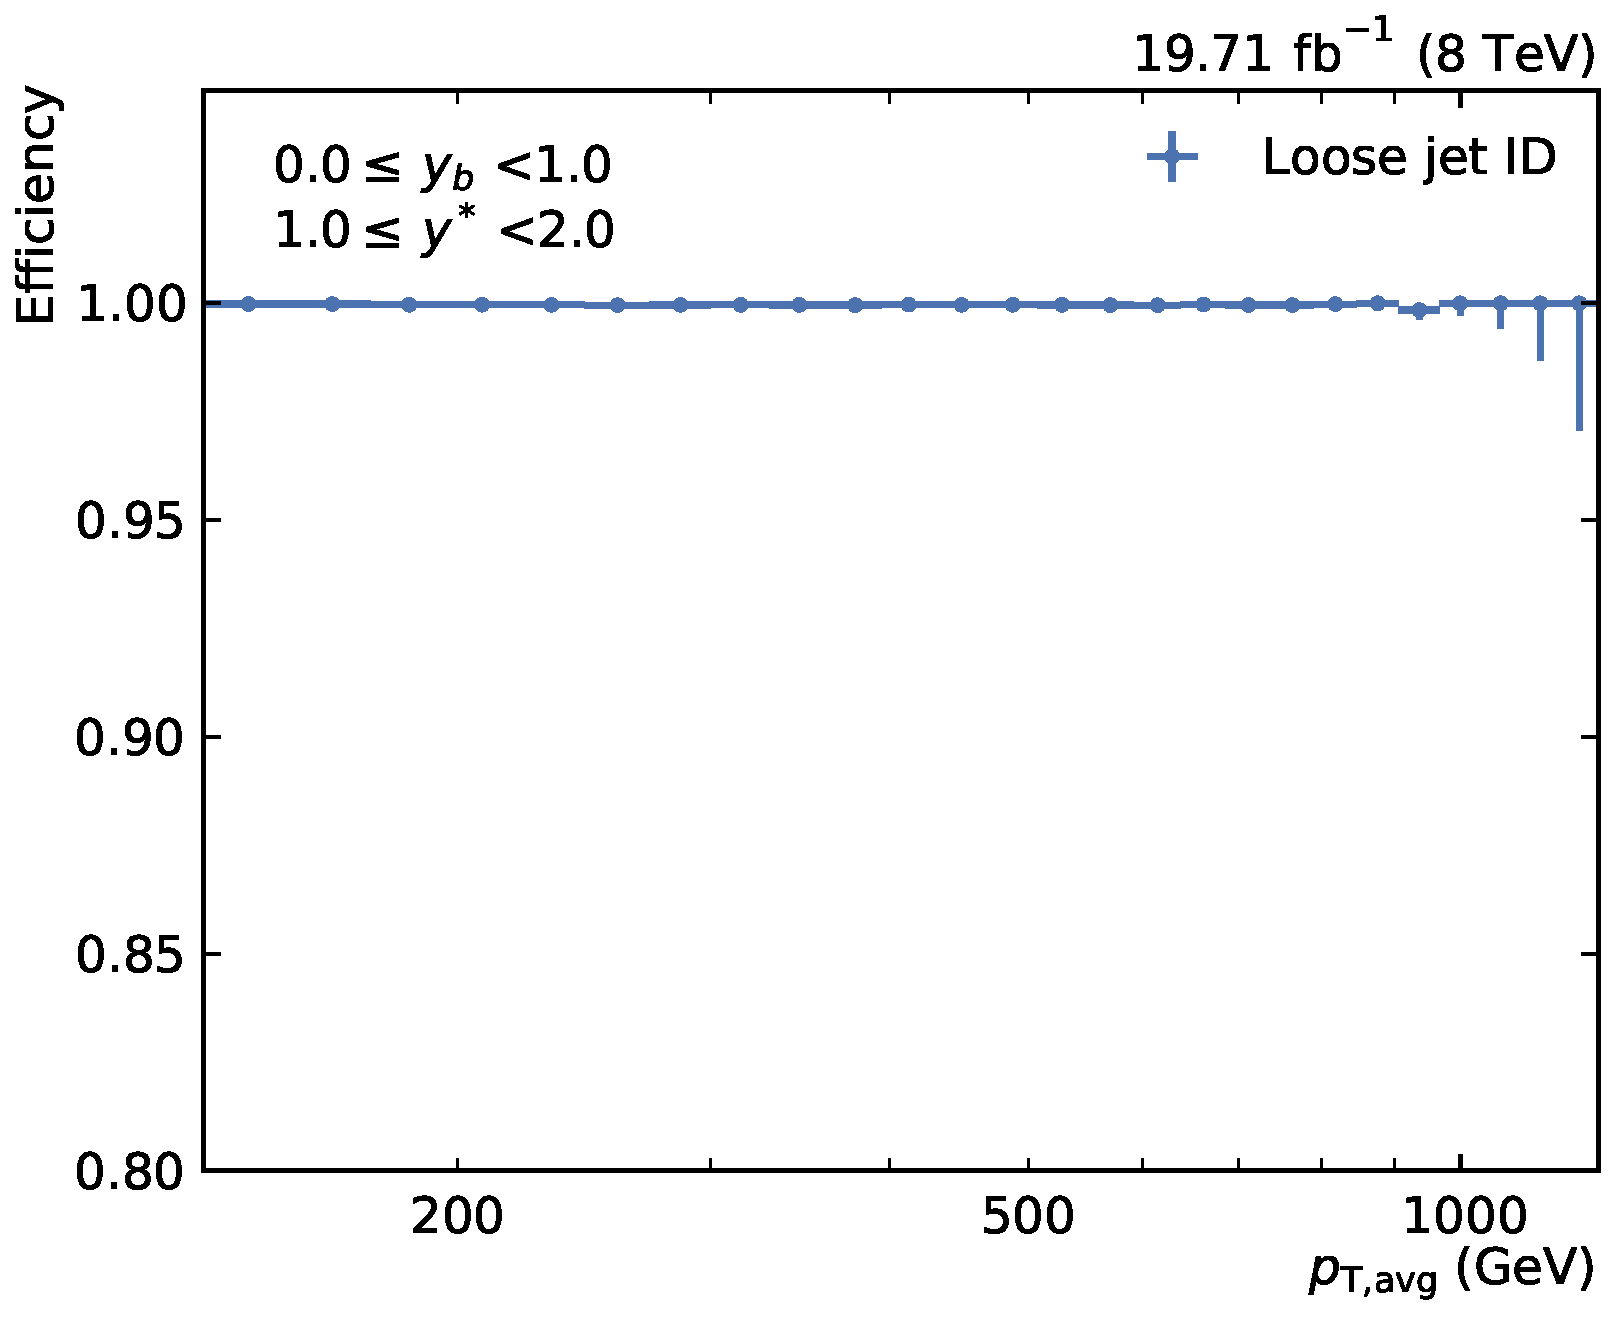
\includegraphics[width=0.49\textwidth]{figures/measurement/jetideff_yb0ys1.pdf}
    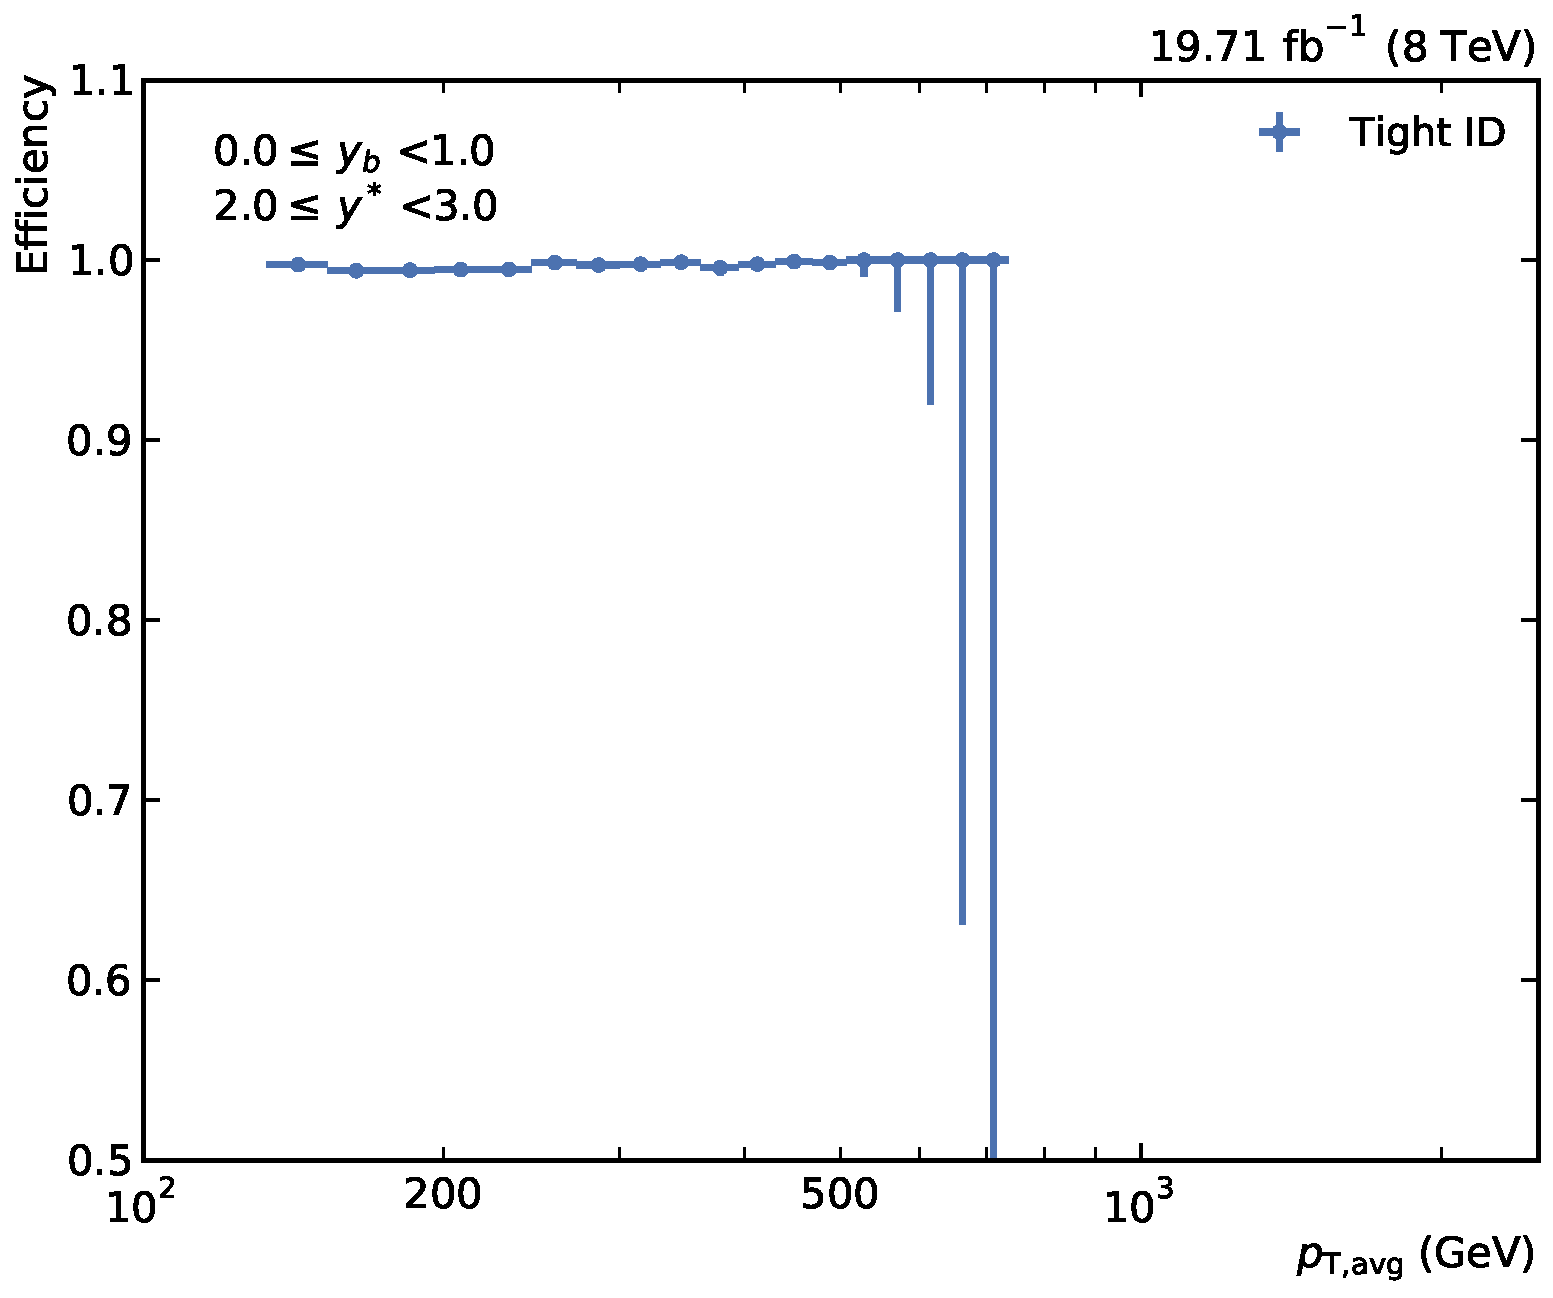
\includegraphics[width=0.49\textwidth]{figures/measurement/jetideff_yb0ys2.pdf}\hfill
    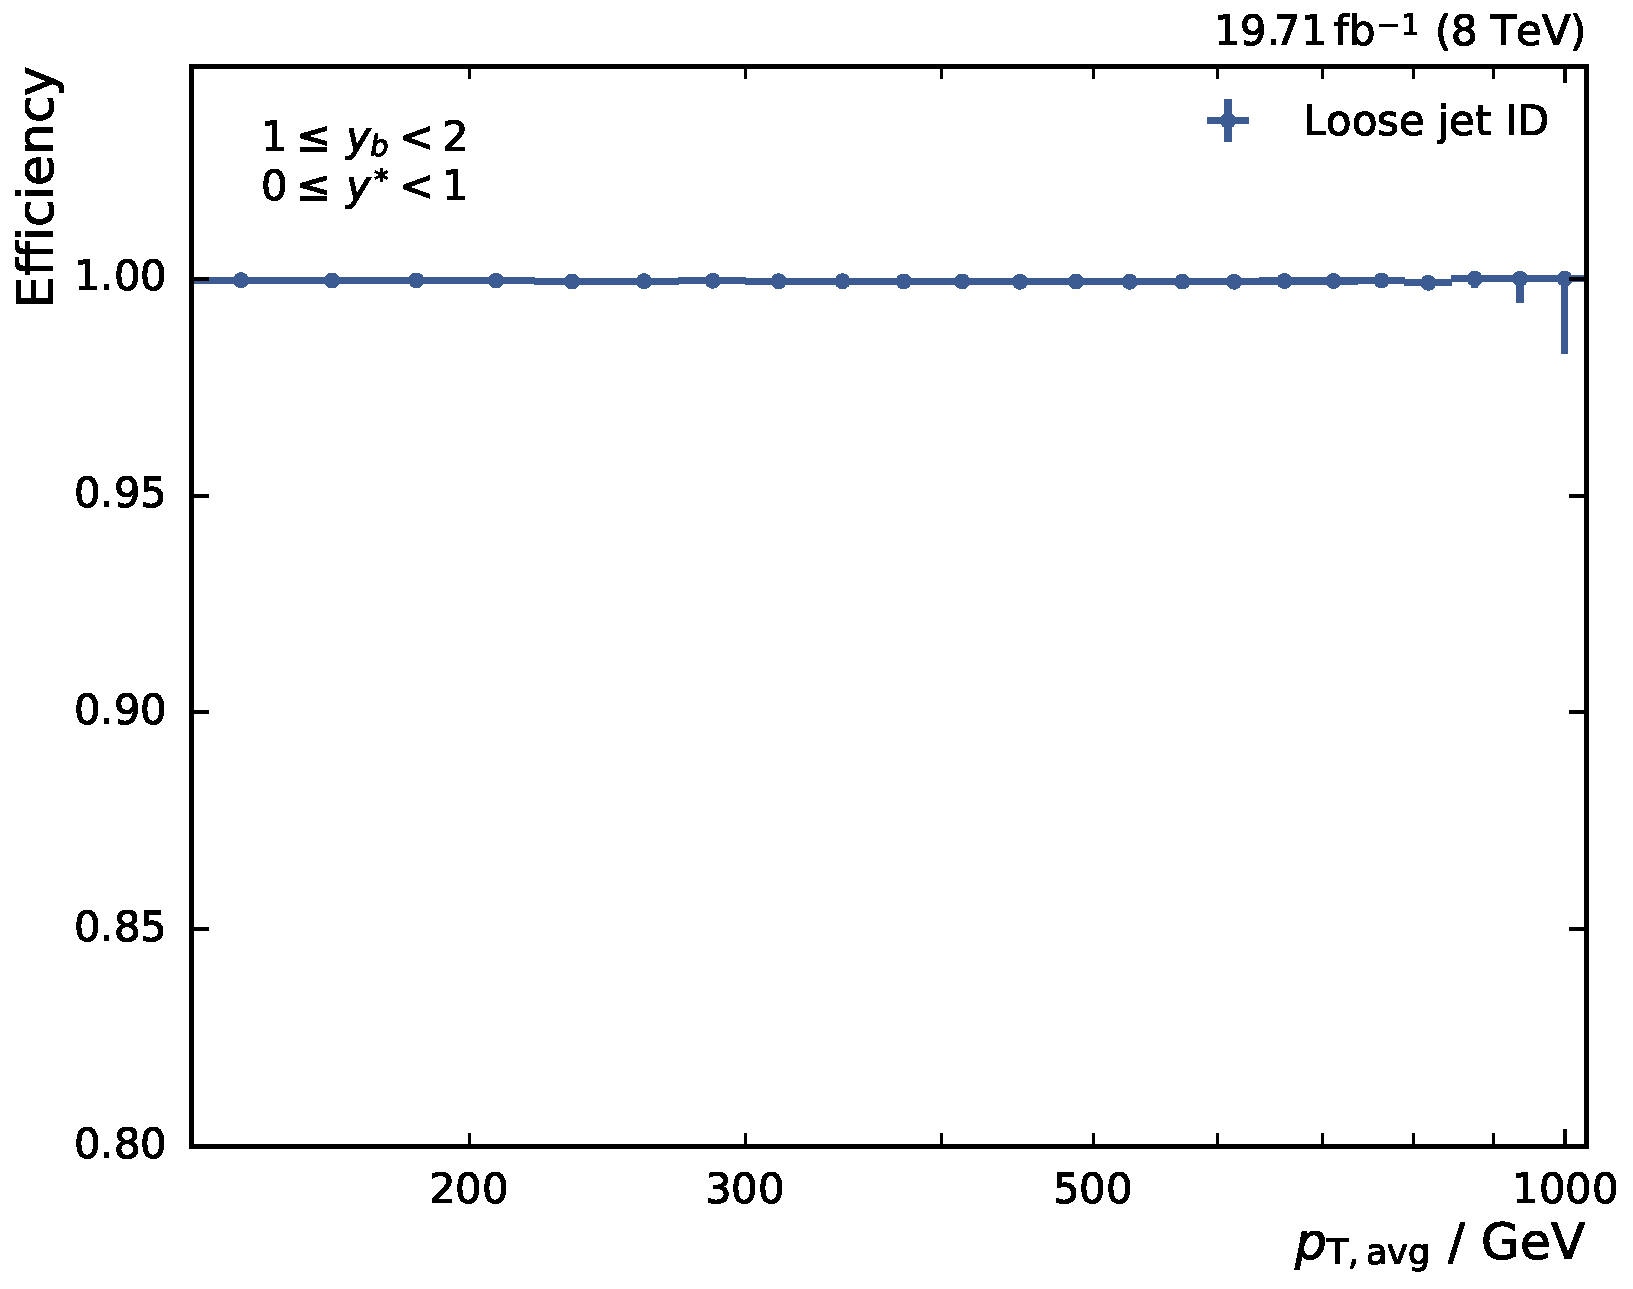
\includegraphics[width=0.49\textwidth]{figures/measurement/jetideff_yb1ys0.pdf}
    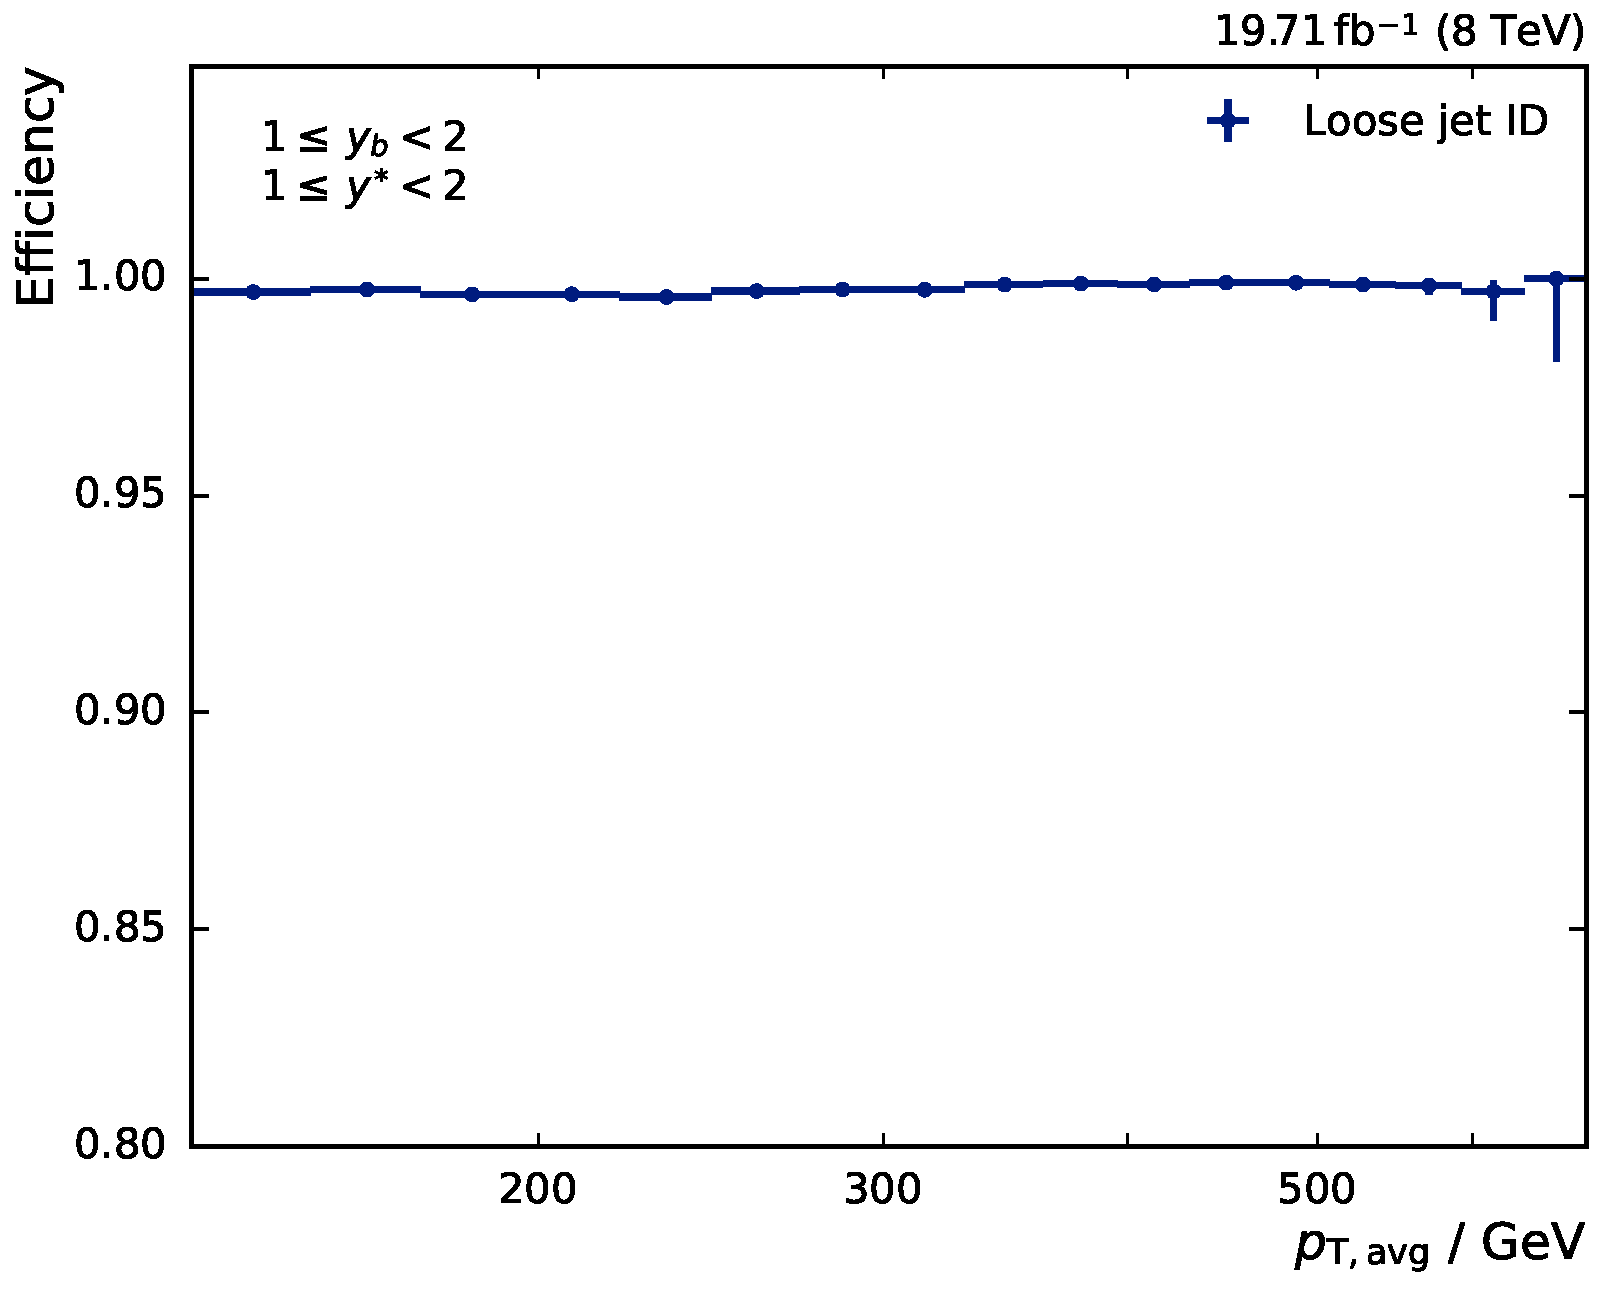
\includegraphics[width=0.49\textwidth]{figures/measurement/jetideff_yb1ys1.pdf}\hfill
    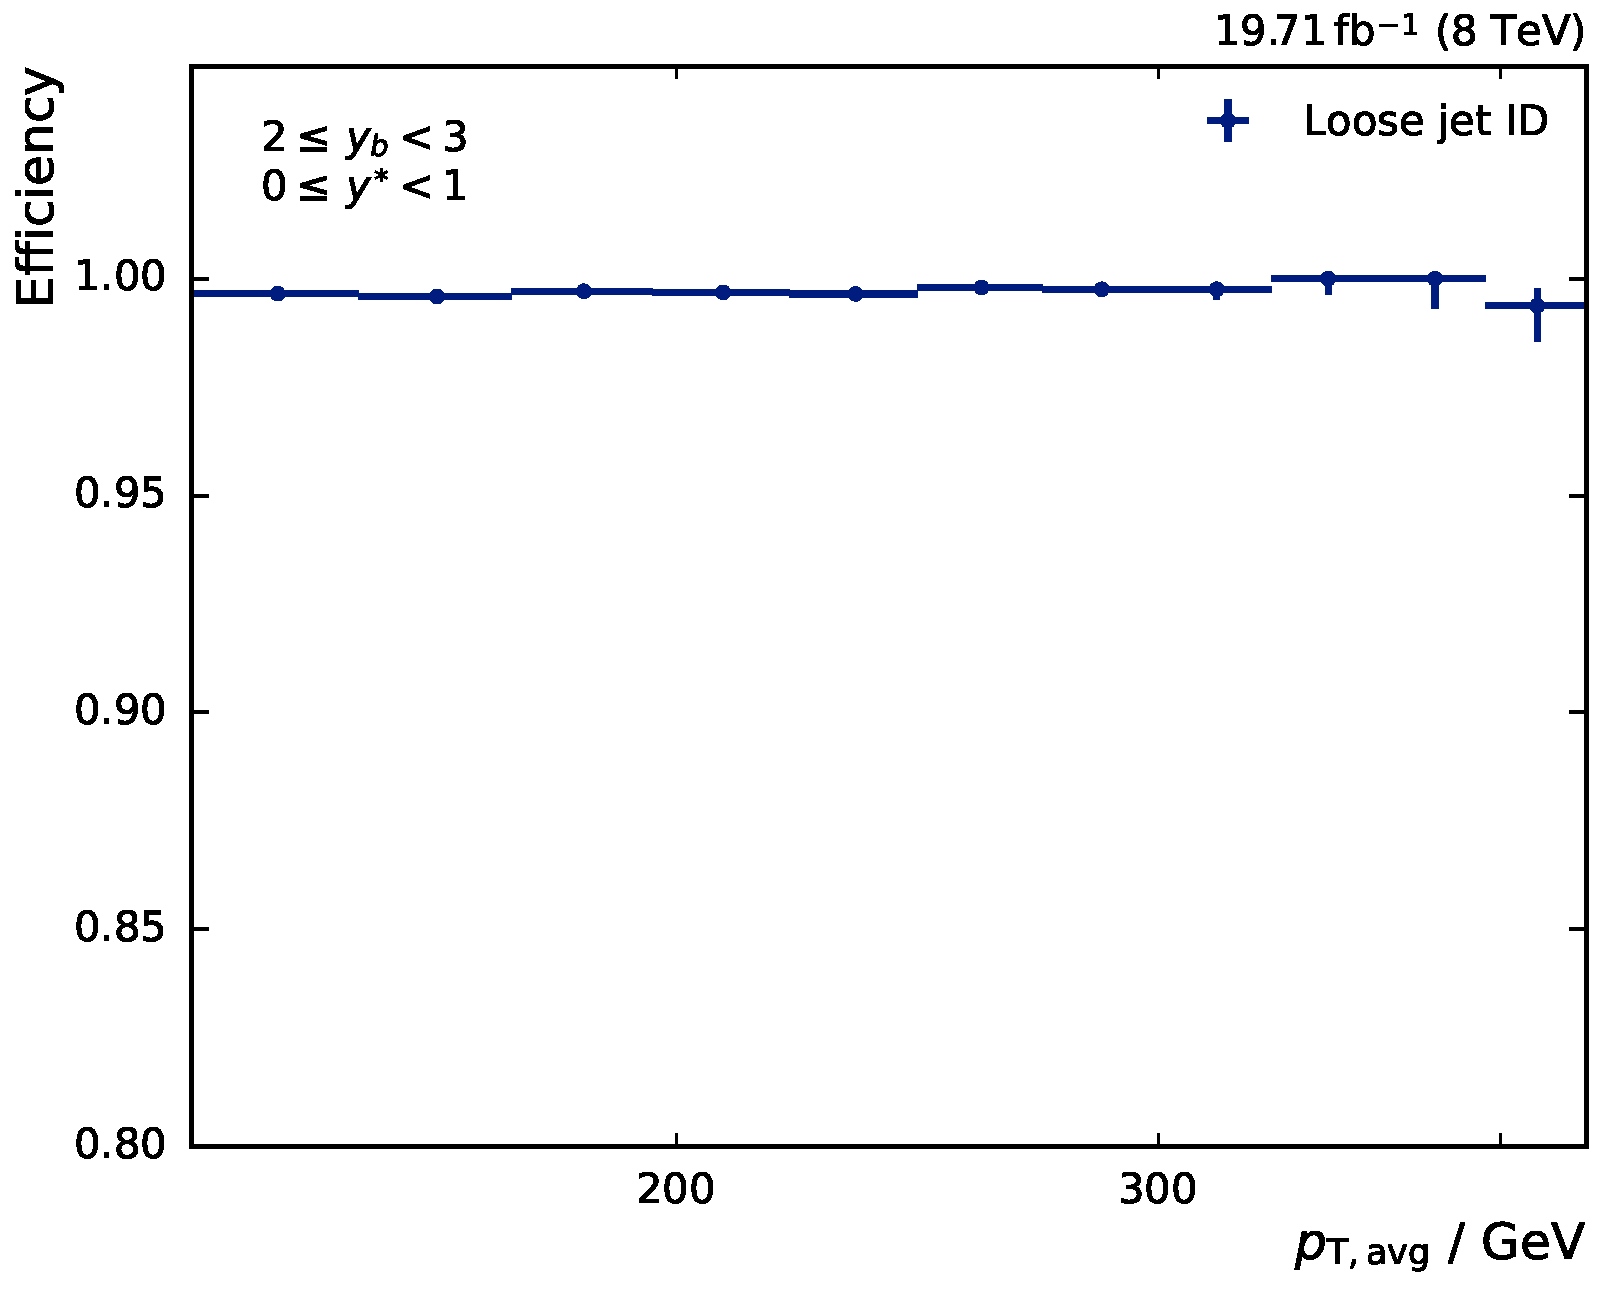
\includegraphics[width=0.49\textwidth]{figures/measurement/jetideff_yb2ys0.pdf}
    \caption[Efficiency of the jet ID]{The jet ID efficiency as a function of
    \ptavg for all \ystar and \yboost bins. It is studied using a
    tag-and-probe approach on dijet event topologies. The efficiency is
    shown as a function of \ptavg for all bins. It always exceeds \SI{99}{\percent}.}
    \label{fig:jetid_eff}
\end{figure}

\subsection{Jet Energy Corrections and Selection}

The measurement presented in this thesis is based on jets clustered from PF
candidates using the anti-\kt jet algorithm with a size parameter of 0.7. The
following phase space cuts remove jets instead of whole events due to their
transverse momentum and rapidity. Consequently, all jet energy corrections
recommended by CMS are applied prior to this selection in order to have the
correct energy scale of the jets. The factorized correction approach employed by
CMS is discussed in Sec.~\ref{sec:jec} and comprises different correction levels
for jets in data\footnote{The JEC version applied on data is internally referred
to as \texttt{Winter14\_V8}} and for jets in simulated events\footnote{The
latest JEC for run-independent Monte Carlo Samples are called
\texttt{START53\_V27}}.

The accessible phase space in theoretical calculations and in the measurement is
synchronized by selecting jets only from a restricted part of the complete phase
space, in which the detector acceptance is high and the applicability of NLO
pQCD calculations is guaranteed:
%
\begin{align*}
    \ptjet &> \SI{50}{\GeV}\\
    |y_\mathrm{jet}| &\leq 3.0\\
\end{align*}
%
Events in which the leading or second jet fail the jet selection are
discarded in order to only keep events in which both leading jets stem
from the hard scattering. Furthermore, an additional cut on the
average transverse momentum of the dijets is applied:
%
\begin{align*}
    \ptavg &> \SI{133}{\GeV}
\end{align*}
%
This cut is necessary, as the first employed single jet trigger becomes
efficient at this point. Often, it is recommended to have asymmetric cuts on the
transverse momentum of the two leading jets to avoid an infrared sensitive
region. Because of the much higher cut on the average transverse momentum, this
is not an issue here. Other advantages of the high cut on \ptavg are the
avoidance of a turn-on region which would lead to complications in the applied
unfolding procedure as well as the restriction to a phase space region in which
non-perturbative contributions are small.

\subsection{Angular Jet Corrections}

The jet energy corrections relate the reconstructed jet energy to the particle-level jet energy, but they do not include any correction for angular
reconstruction biases of the jets. However, especially in the transitional
regions of the detector, \ie when the tracker coverage ends, a systematic
reconstruction bias is observed, see Fig.~\ref{fig:jet_eta_corr}. Jets are
reconstructed with systematically larger absolute pseudorapidity, meaning they
are shifted towards the forward region. While the absolute shift is rather
small, it causes a relevant systematic effect whenever the rapidity separation
of two jets is of interest. There are two effects however, that limit the impact of the
misreconstruction: First, it is only pronounced for jets with low transverse momentum
(as can be seen in Fig~\ref{fig:jet_eta_corr_vs_pt}) and second, the large bin
size in \ystar and \yboost used in this analysis reduces the impact. 

Nonetheless, the systematic bias is accounted for by applying a correction on
each jet based on the average difference between the pseudorapidity of
particle-level jets and reconstructed jets as a function of reconstructed jet
\pt and pseudorapidity. The Figs.~\ref{fig:jet_eta_corr}
and~\ref{fig:jet_eta_corr_vs_pt} also show the distribution after applying the
correction, in which the majority of the $\eta$-dependent effects is removed.

\begin{figure}[htbp]
    \centering
    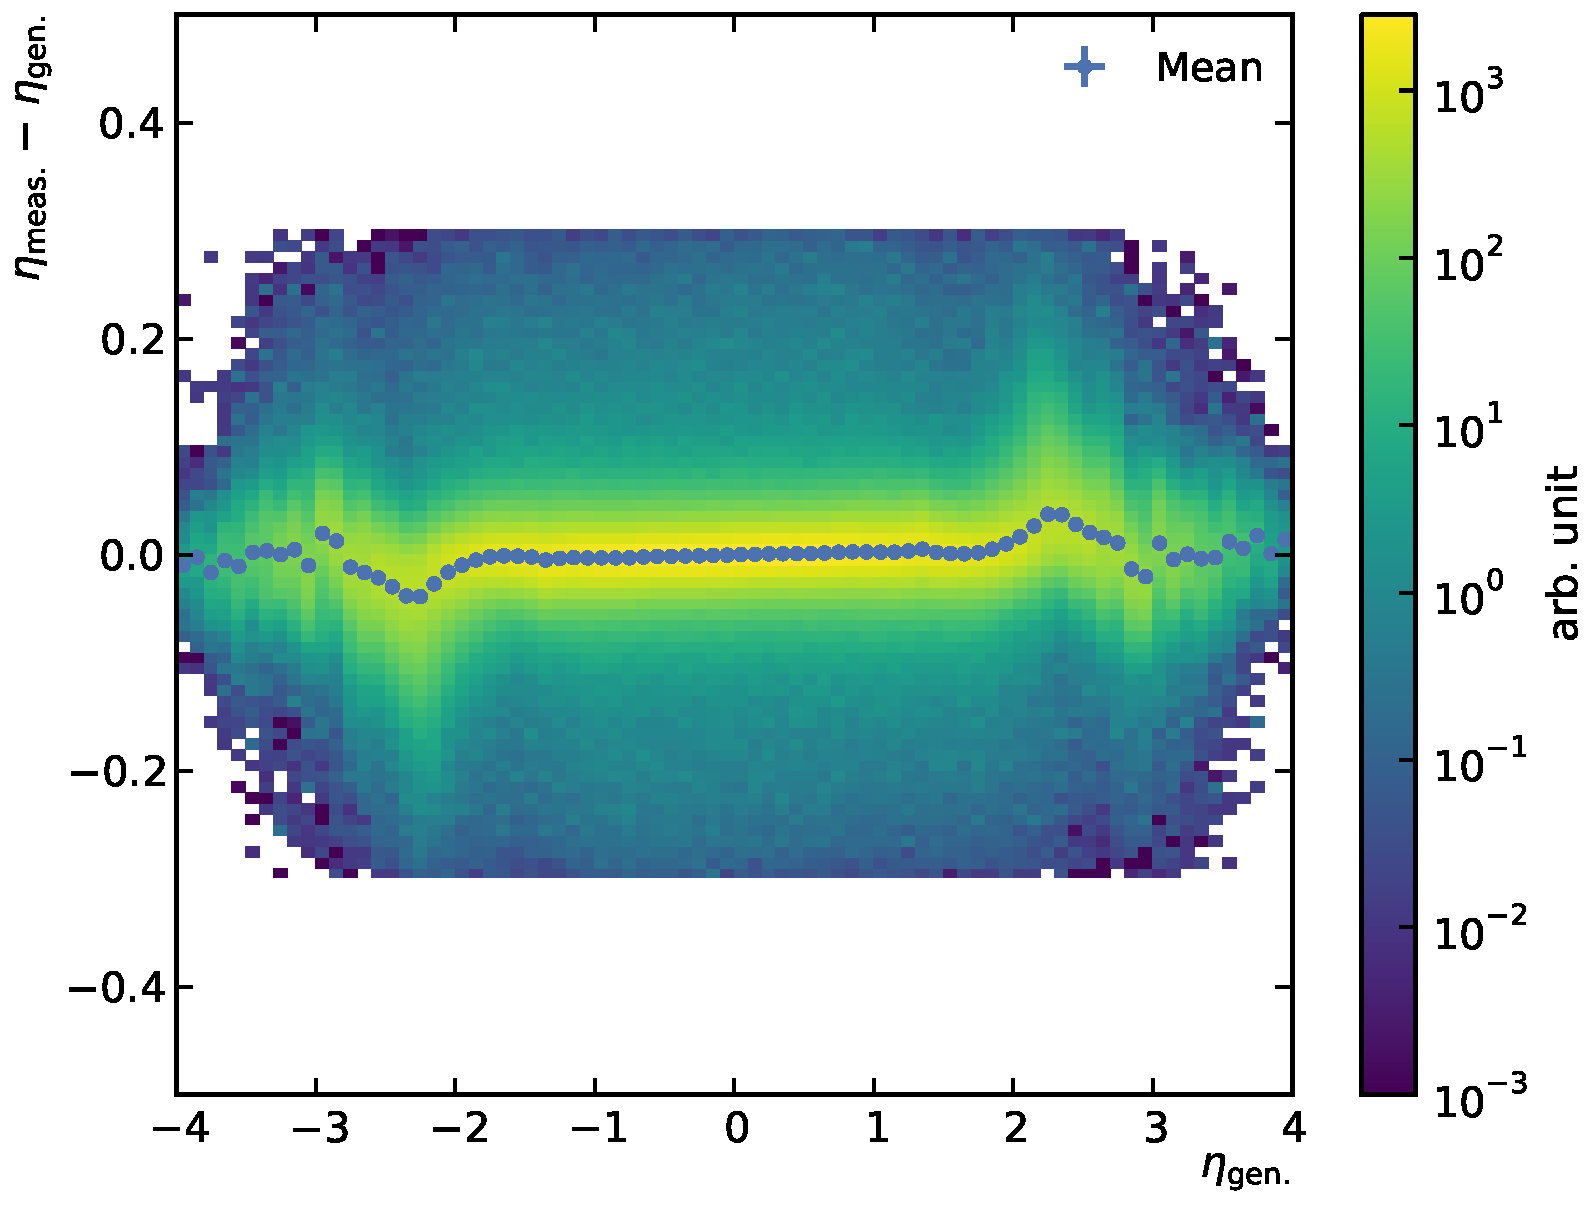
\includegraphics[width=0.49\textwidth]{figures/measurement/genvsreco_eta.pdf}\hfill
    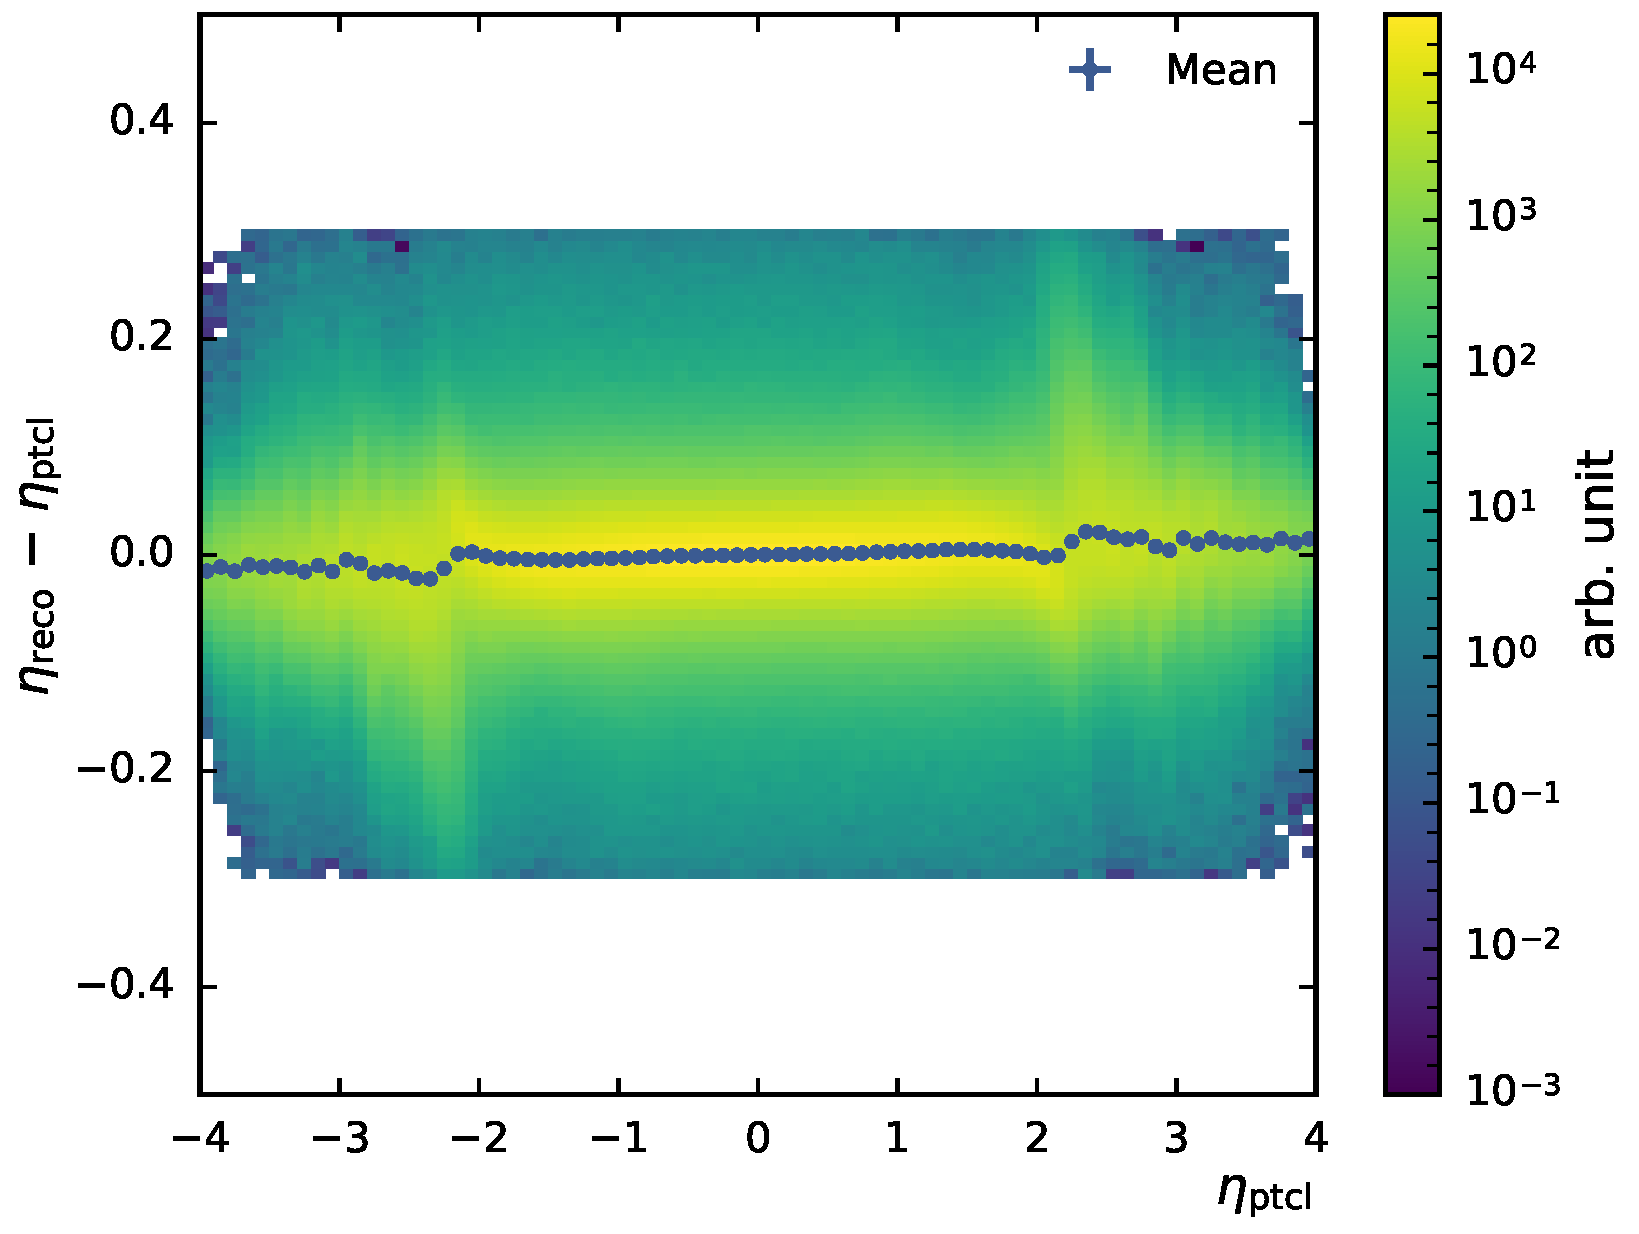
\includegraphics[width=0.49\textwidth]{figures/measurement/genvsreco_eta_corr.pdf}
    \caption[Differences of pseudorapidity of reconstructed jets to
        particle-level jets]{The difference between the pseudorapidity of the
            reconstructed jets and the generated jets is shown over the
            pseudorapidity of the generated jet. The distribution is shown
            before (left) and after (right) applying the pseudorapidity
            correction. The blue points indicate the mean of the distribution in
            each $\eta_{\mathrm{gen}}$ bin.}
    \label{fig:jet_eta_corr}
\end{figure}


\begin{figure}[htbp]
    \centering
    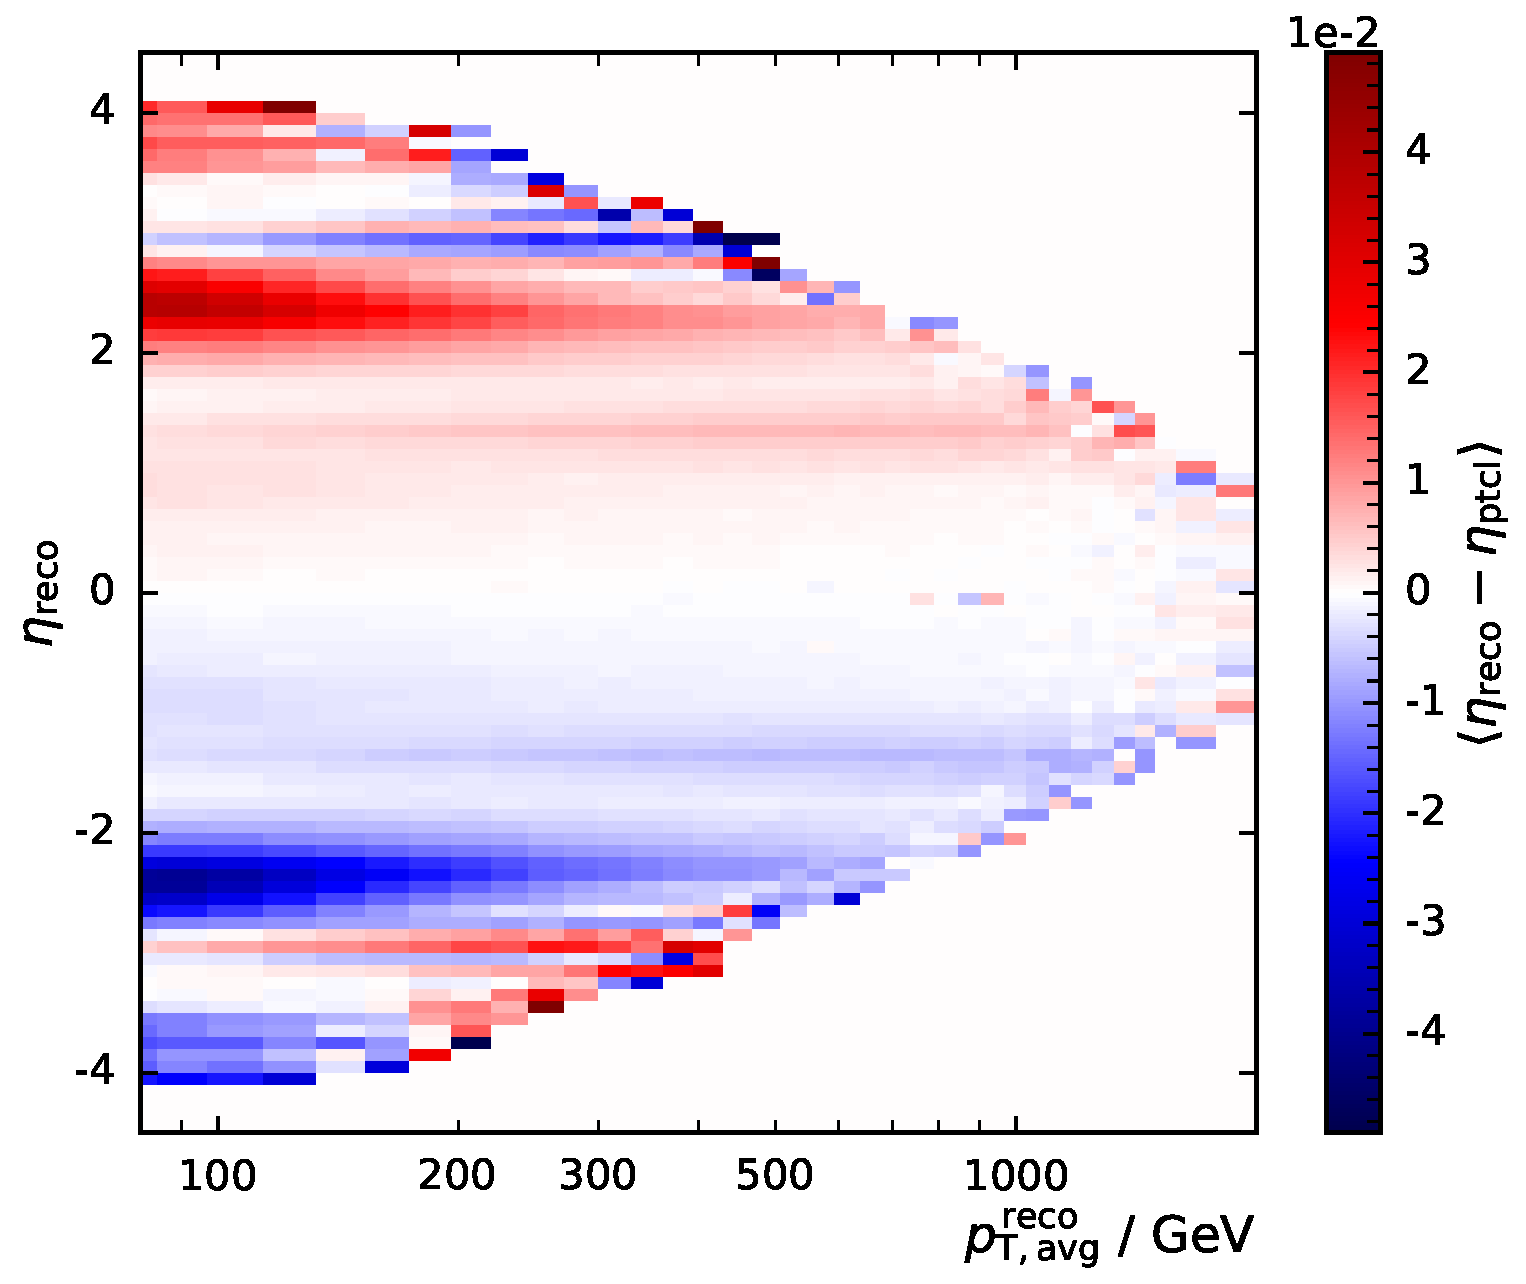
\includegraphics[width=0.49\textwidth]{figures/measurement/genvsreco_eta_vs_genpt.pdf}\hfill
    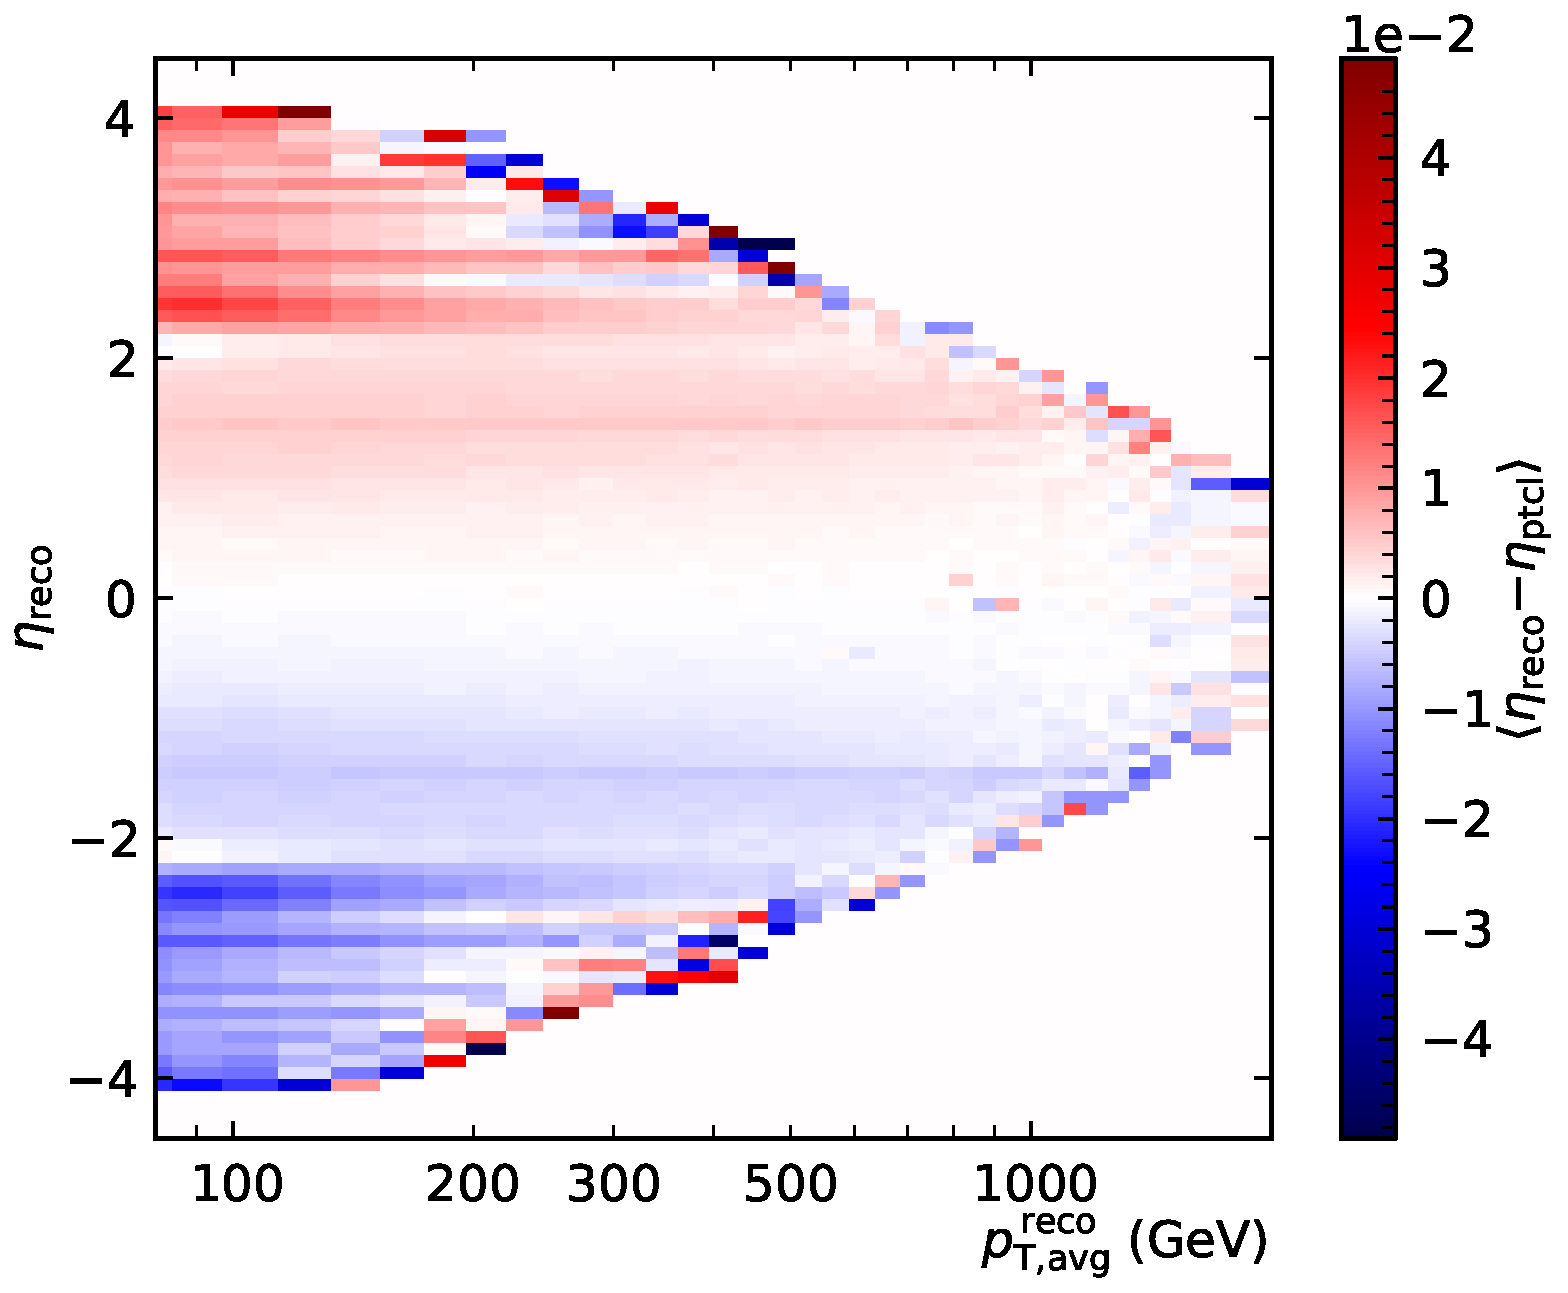
\includegraphics[width=0.49\textwidth]{figures/measurement/genvsreco_eta_vs_genpt_corr.pdf}
    \caption[Differences of pseudorapidity of reconstructed jets and particle-level jets as a function of the reconstructed jet \pt]
            {The pseudorapidity of the
            generated jets is shown as a function of the transverse momentum of
            the jets. The color indicates the differences of the pseudorapidity
            of the generated and reconstructed jets. The distribution is shown
            before (left) and after (right) the angular
        correction is applied.}
    \label{fig:jet_eta_corr_vs_pt}
\end{figure}

To estimate the effect on the resulting cross section, a comparison between the
yielded cross section with and without applying the angular correction is
presented in Fig.~\ref{fig:rap_corr_data}. In the bins containing boosted
dijets, the correction causes changes of about \SI{2}{\percent} of the cross
section. Since these events move to bins containing more central jets in which
the cross section is much higher, no change is noticeable there.

\begin{figure}[htbp]
    \centering
    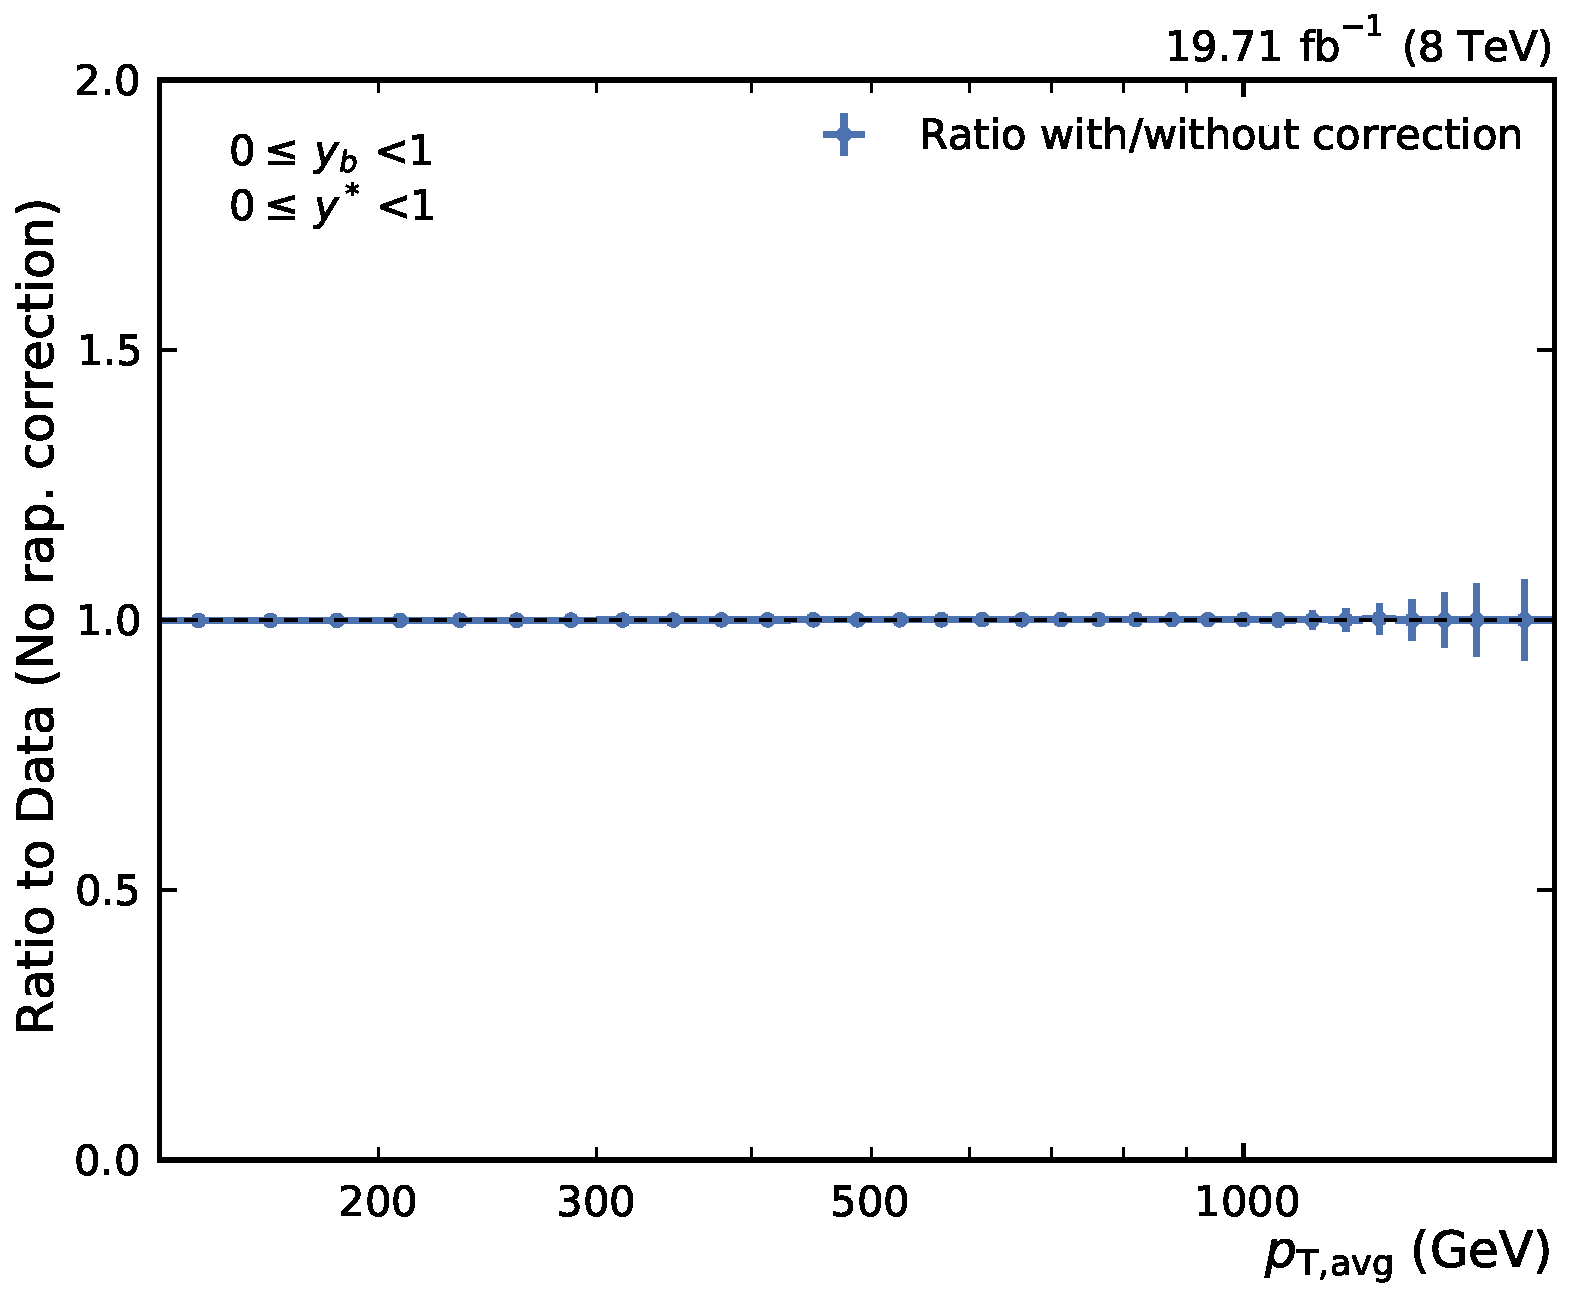
\includegraphics[width=0.47\textwidth]{figures/measurement/rap_corr_data_yb0ys0.pdf}\hfill
    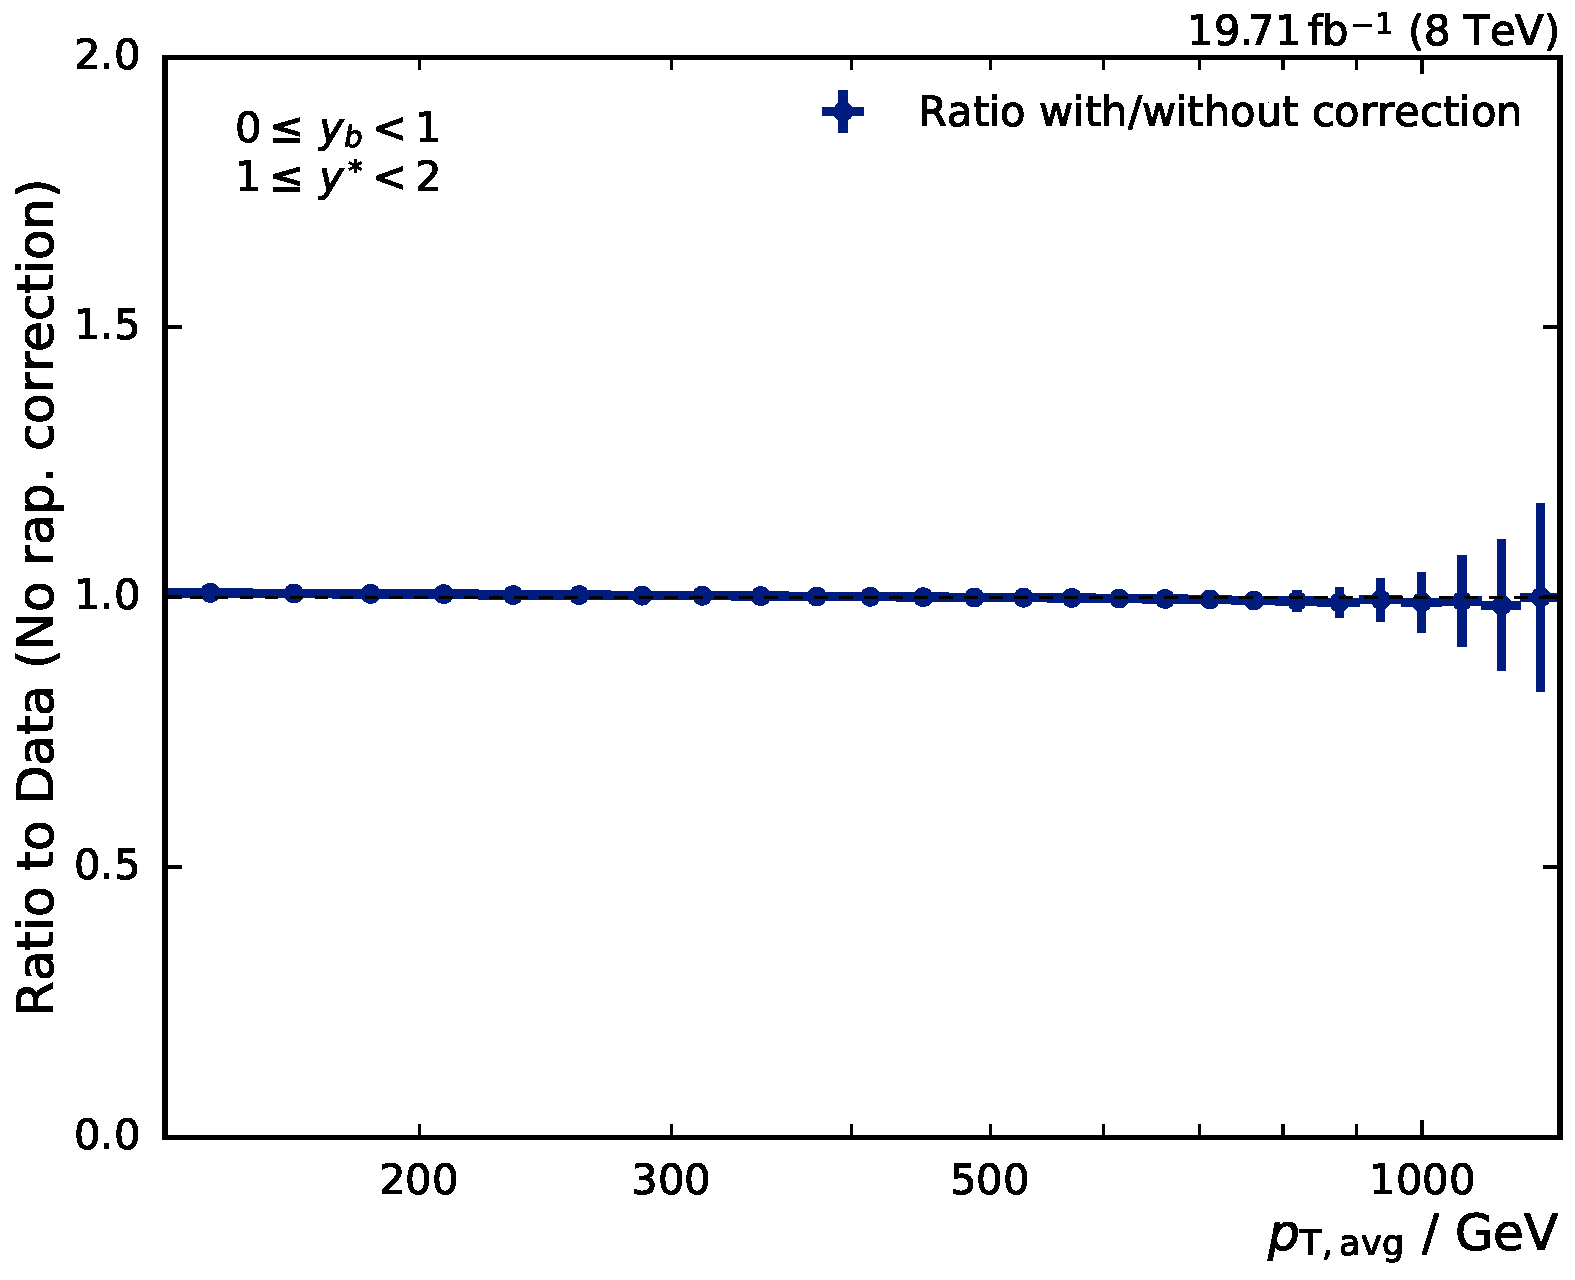
\includegraphics[width=0.47\textwidth]{figures/measurement/rap_corr_data_yb0ys1.pdf}
    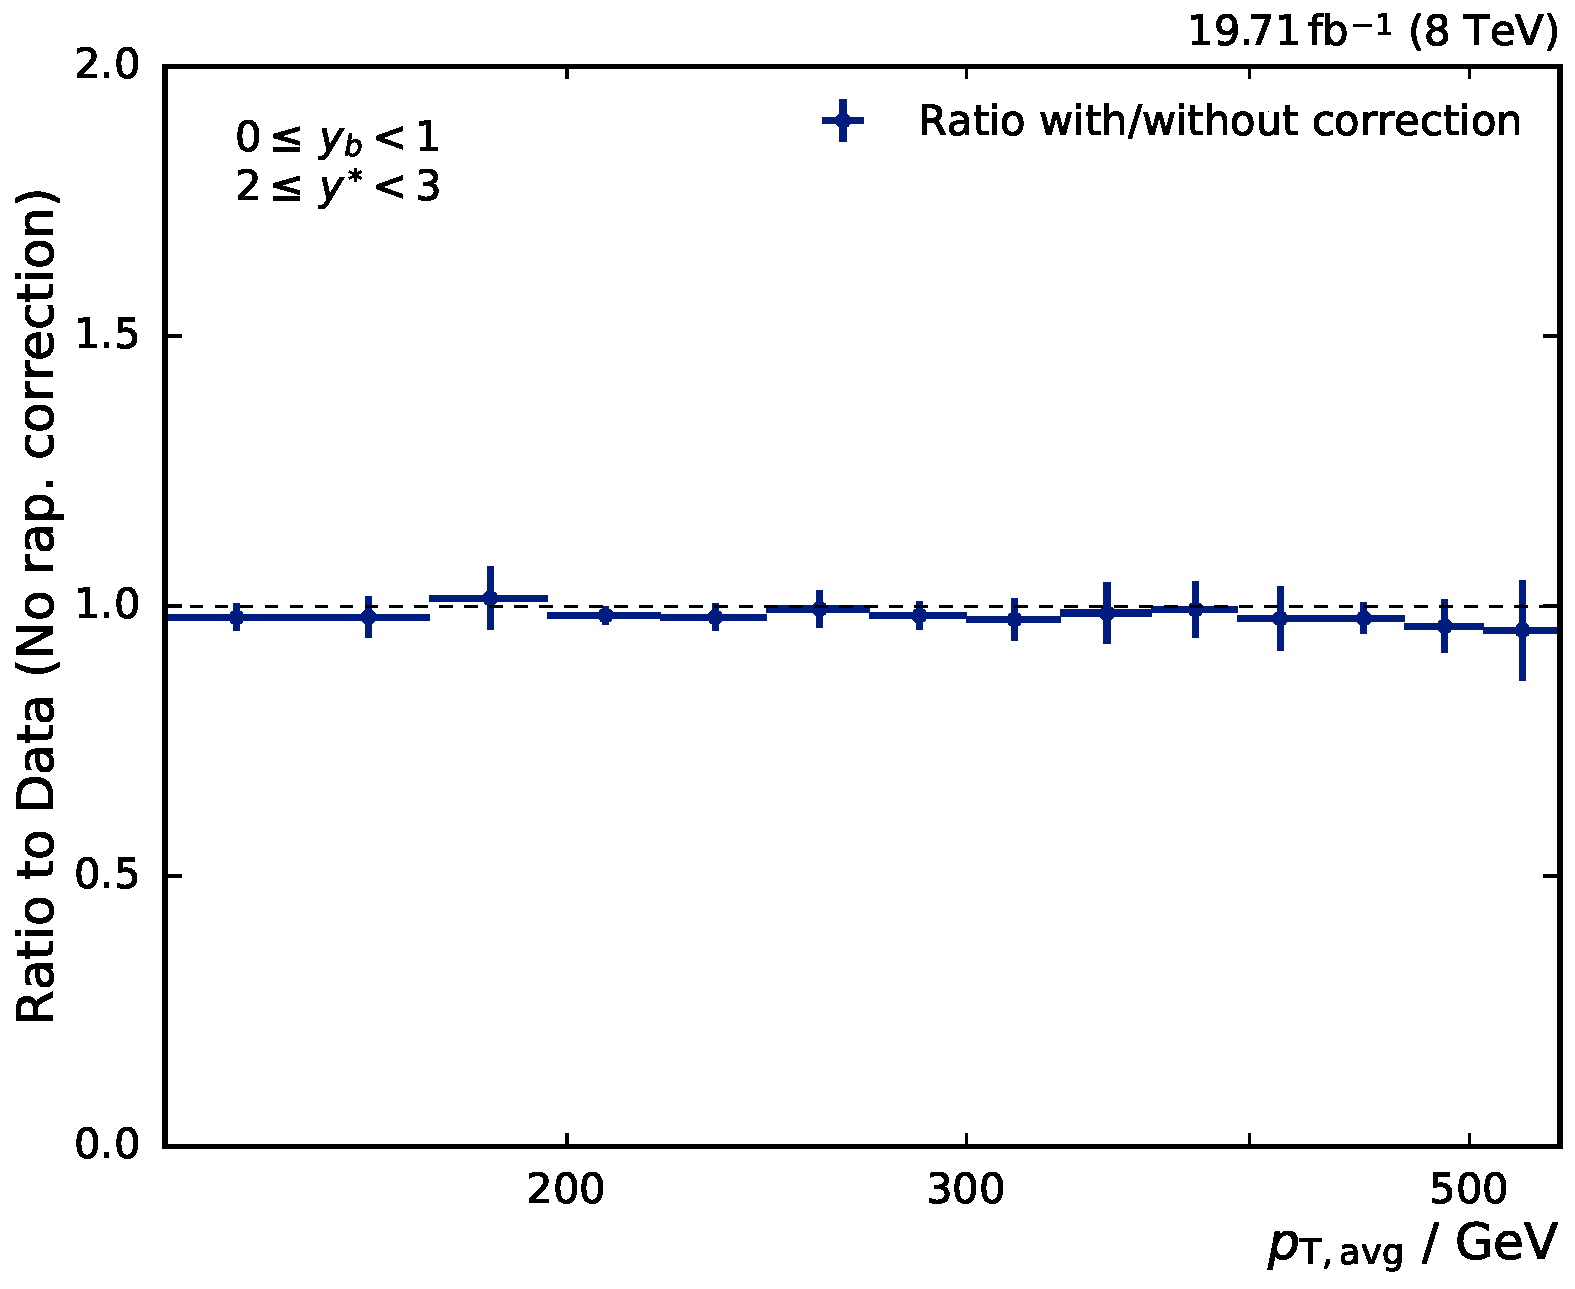
\includegraphics[width=0.47\textwidth]{figures/measurement/rap_corr_data_yb0ys2.pdf}\hfill
    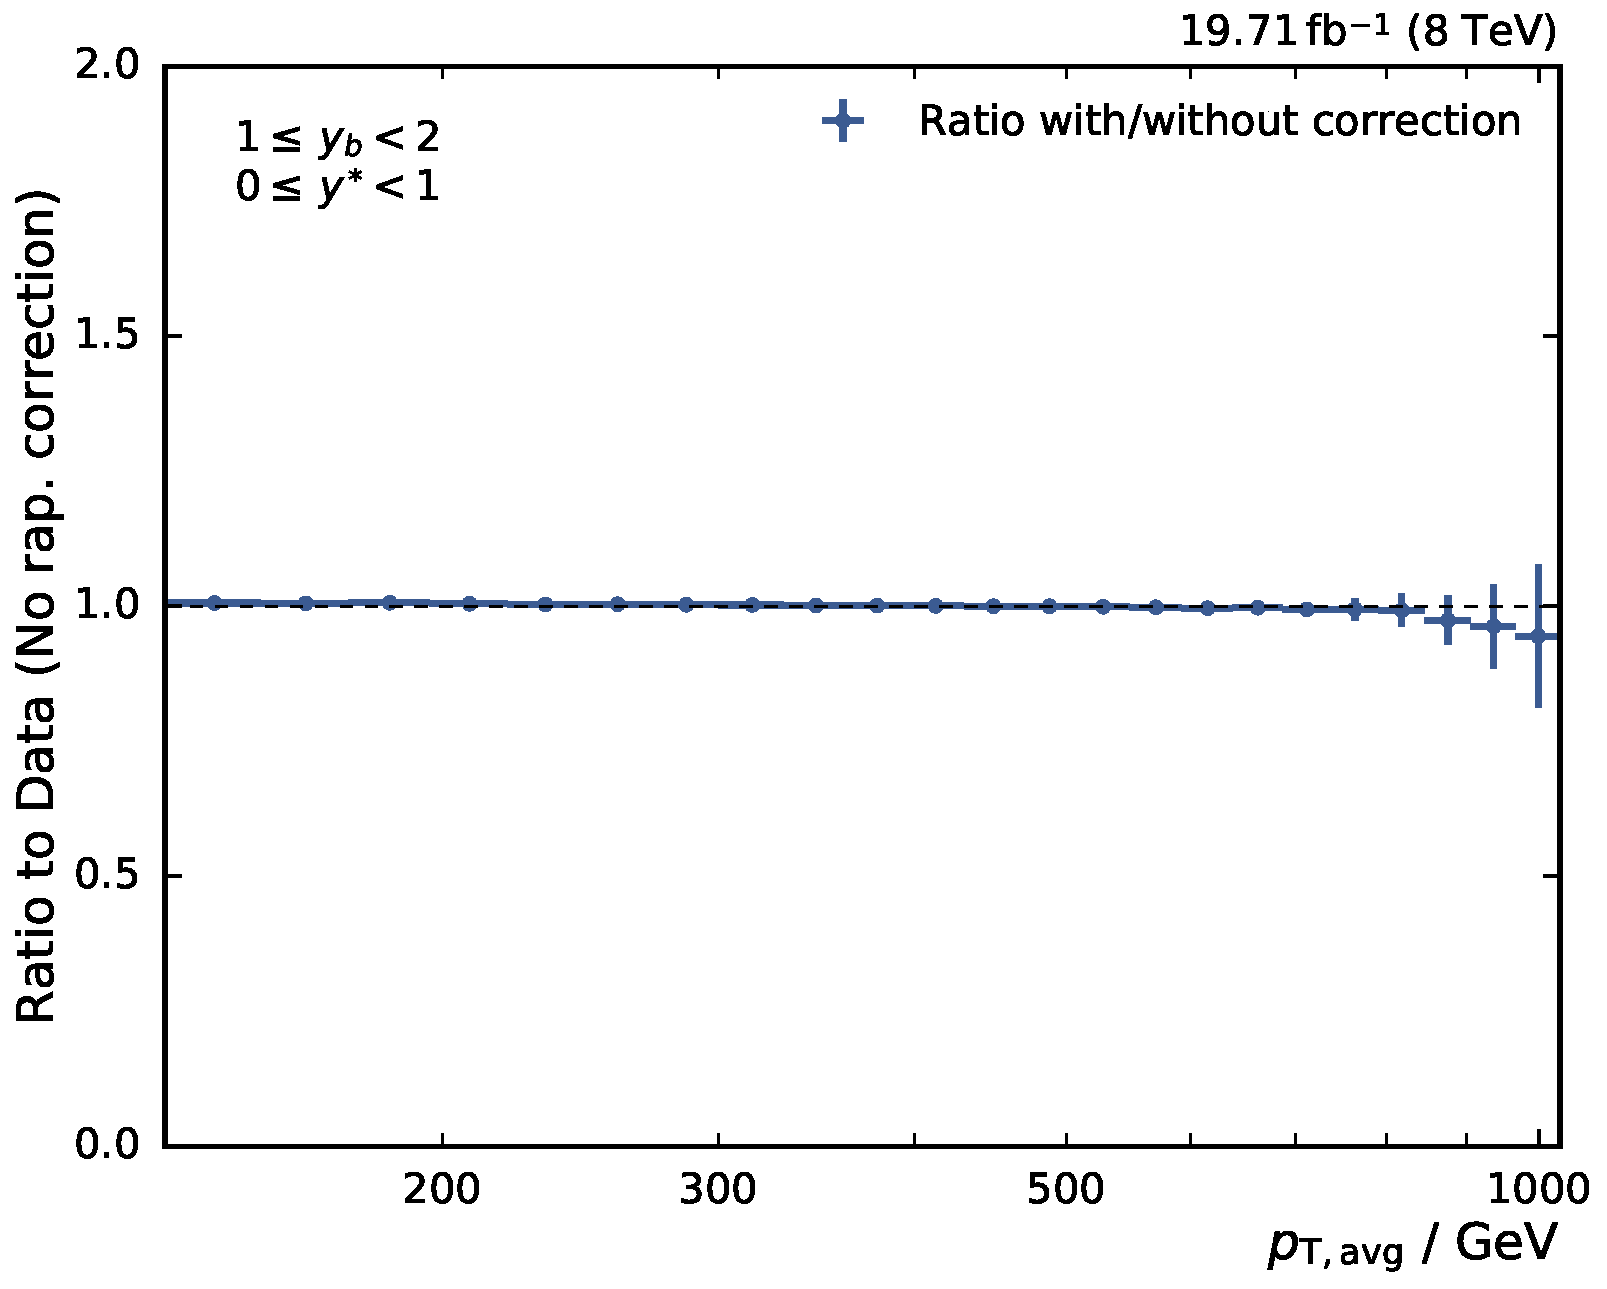
\includegraphics[width=0.47\textwidth]{figures/measurement/rap_corr_data_yb1ys0.pdf}
    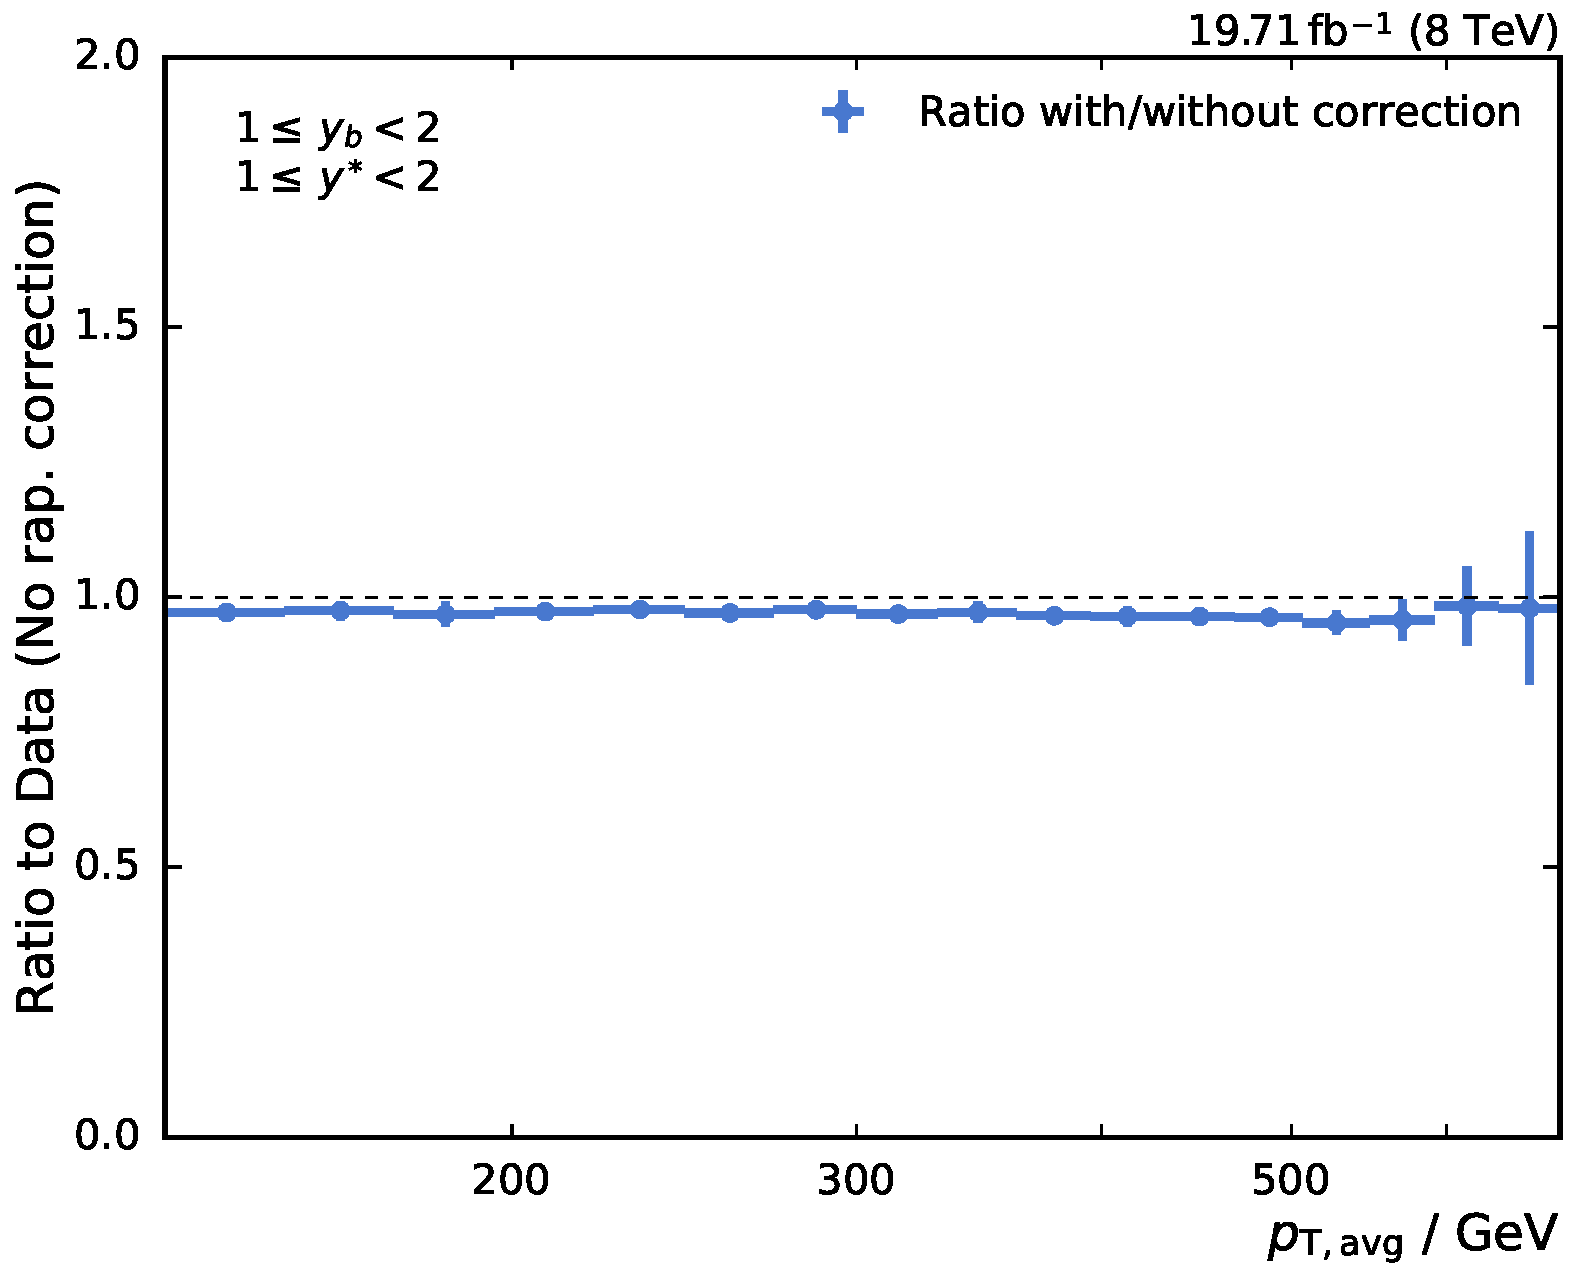
\includegraphics[width=0.47\textwidth]{figures/measurement/rap_corr_data_yb1ys1.pdf}\hfill
    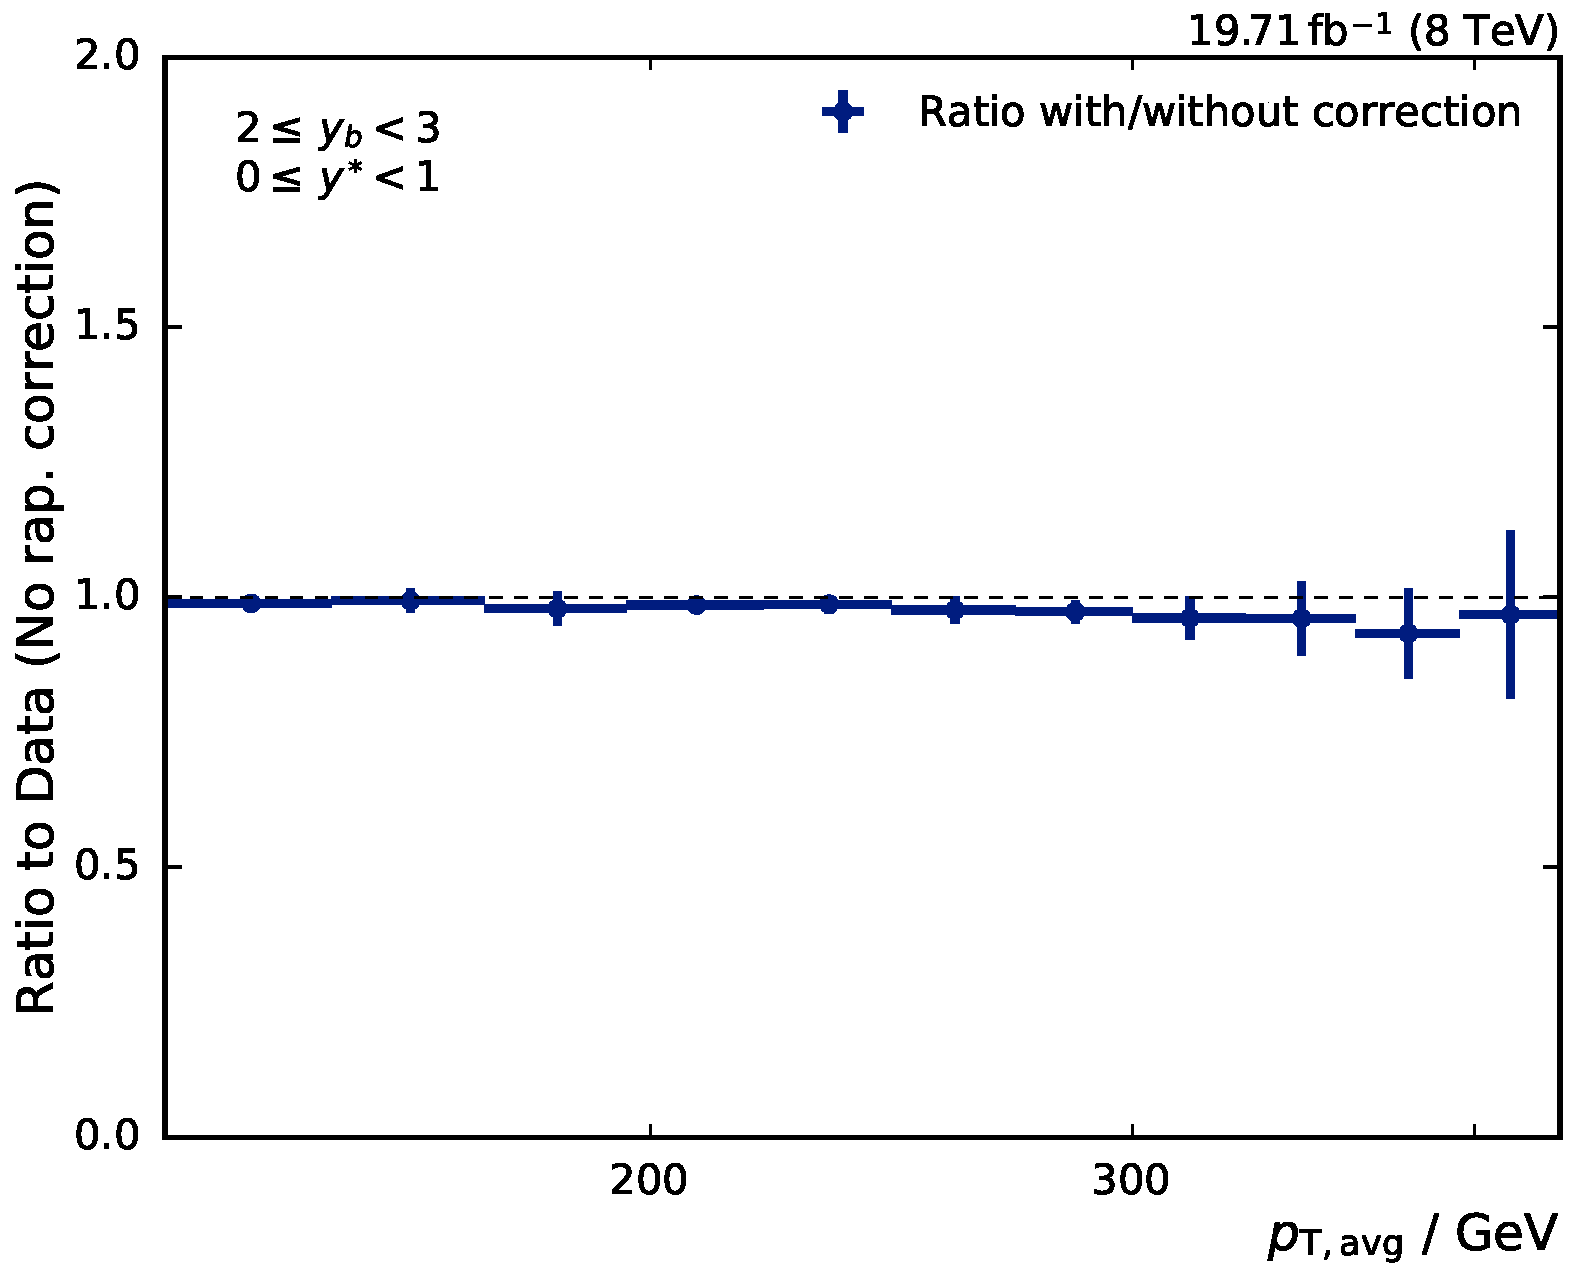
\includegraphics[width=0.47\textwidth]{figures/measurement/rap_corr_data_yb2ys0.pdf}
    \caption[Effect of angular correction]{The effect of the angular correction
        on the cross section  is demonstrated by calculating the ratio of the
        cross section after applying the correction to the one without
        correction. The cross section decreases in bins involving forward jets
        and is more pronounced for higher values of \ystar.}
    \label{fig:rap_corr_data}
\end{figure}

\subsection{Stability versus Run Periods}

The experimental conditions for data-taking change slightly over the various run
periods due to changes of the detector calibration or different trigger
prescales. Nonetheless, the measured cross sections must not depend on
these effects. This is studied by analyzing the different run periods
separately. The result for each run period is shown as ratio to the cross
sections obtained in run D in Fig.~\ref{fig:run_comparison}. 

There are differences visible, most notably due to statistical fluctuations in the
high-\pt region. Furthermore, a slight slope of the cross section obtained in run
B is observed. However, the results are in agreement within uncertainties.

\begin{figure}[htbp]
    \centering
    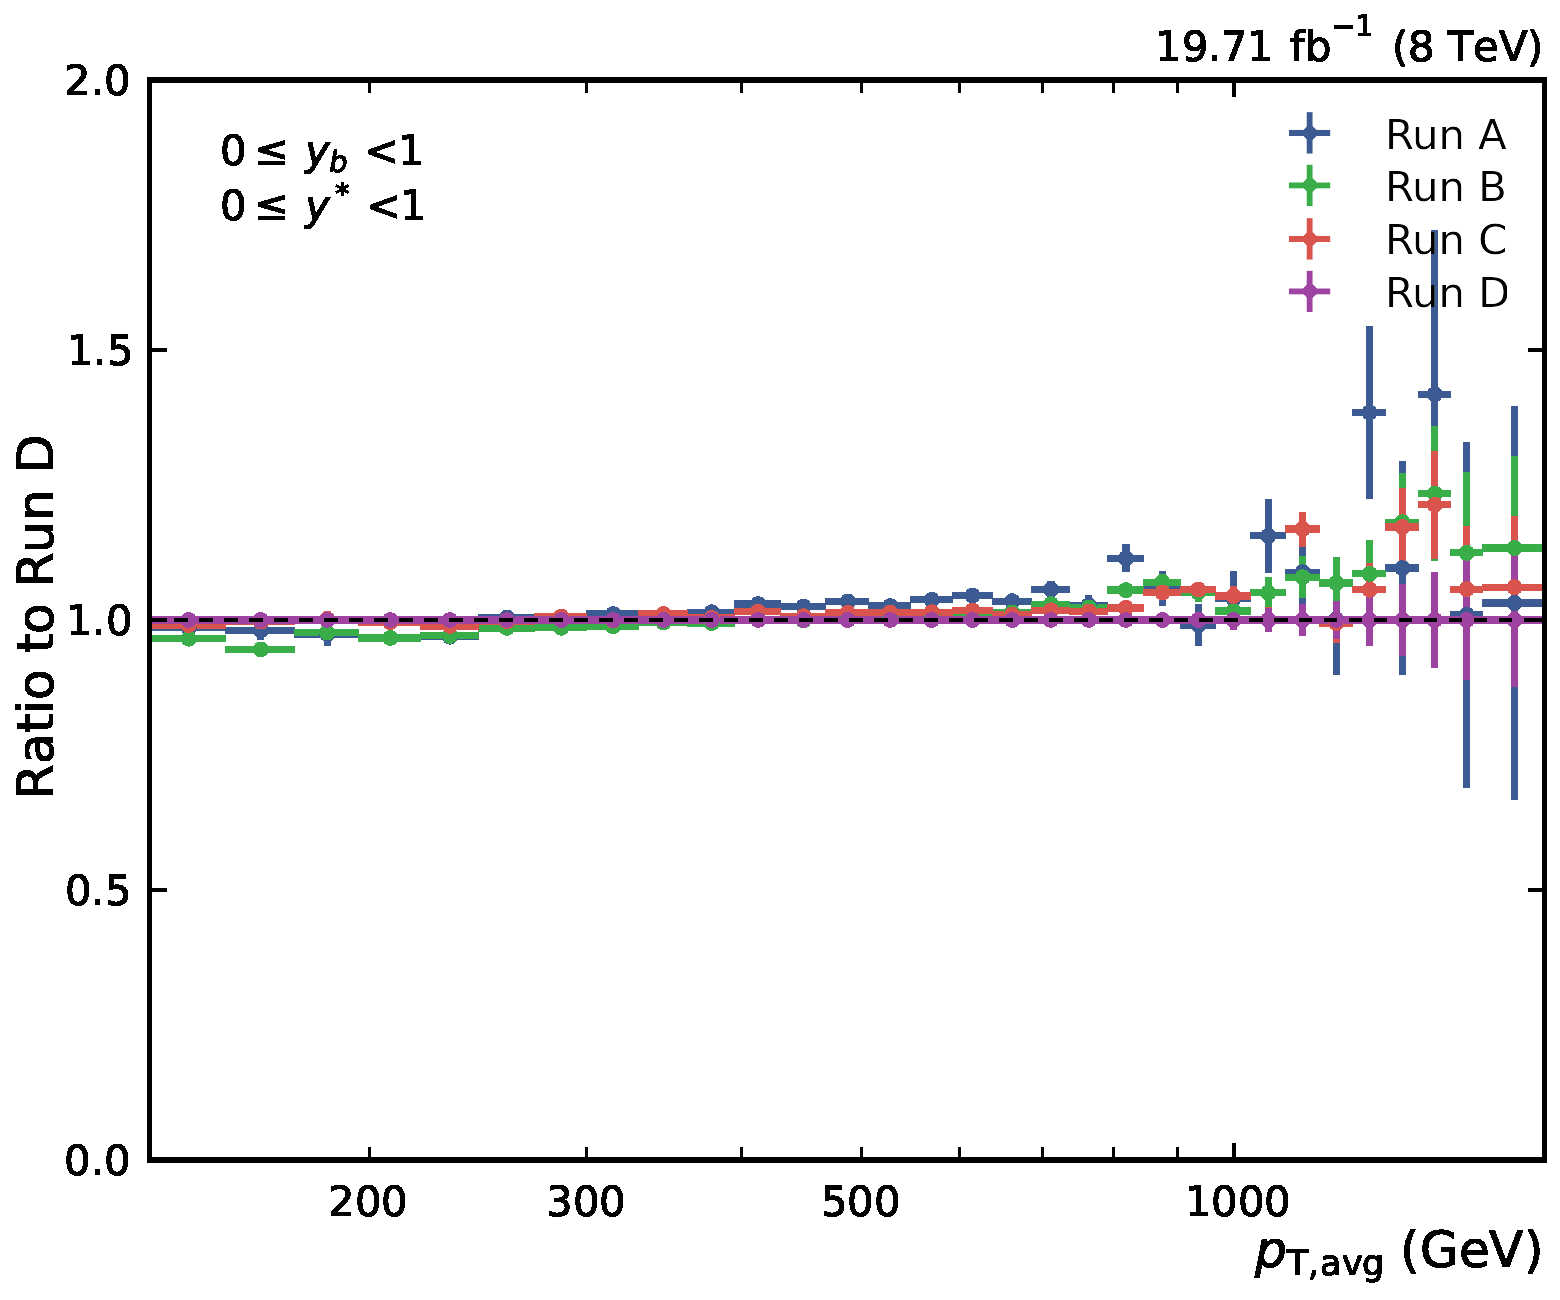
\includegraphics[width=0.47\textwidth]{figures/measurement/run_comparison_yb0ys0.pdf}\hfill
    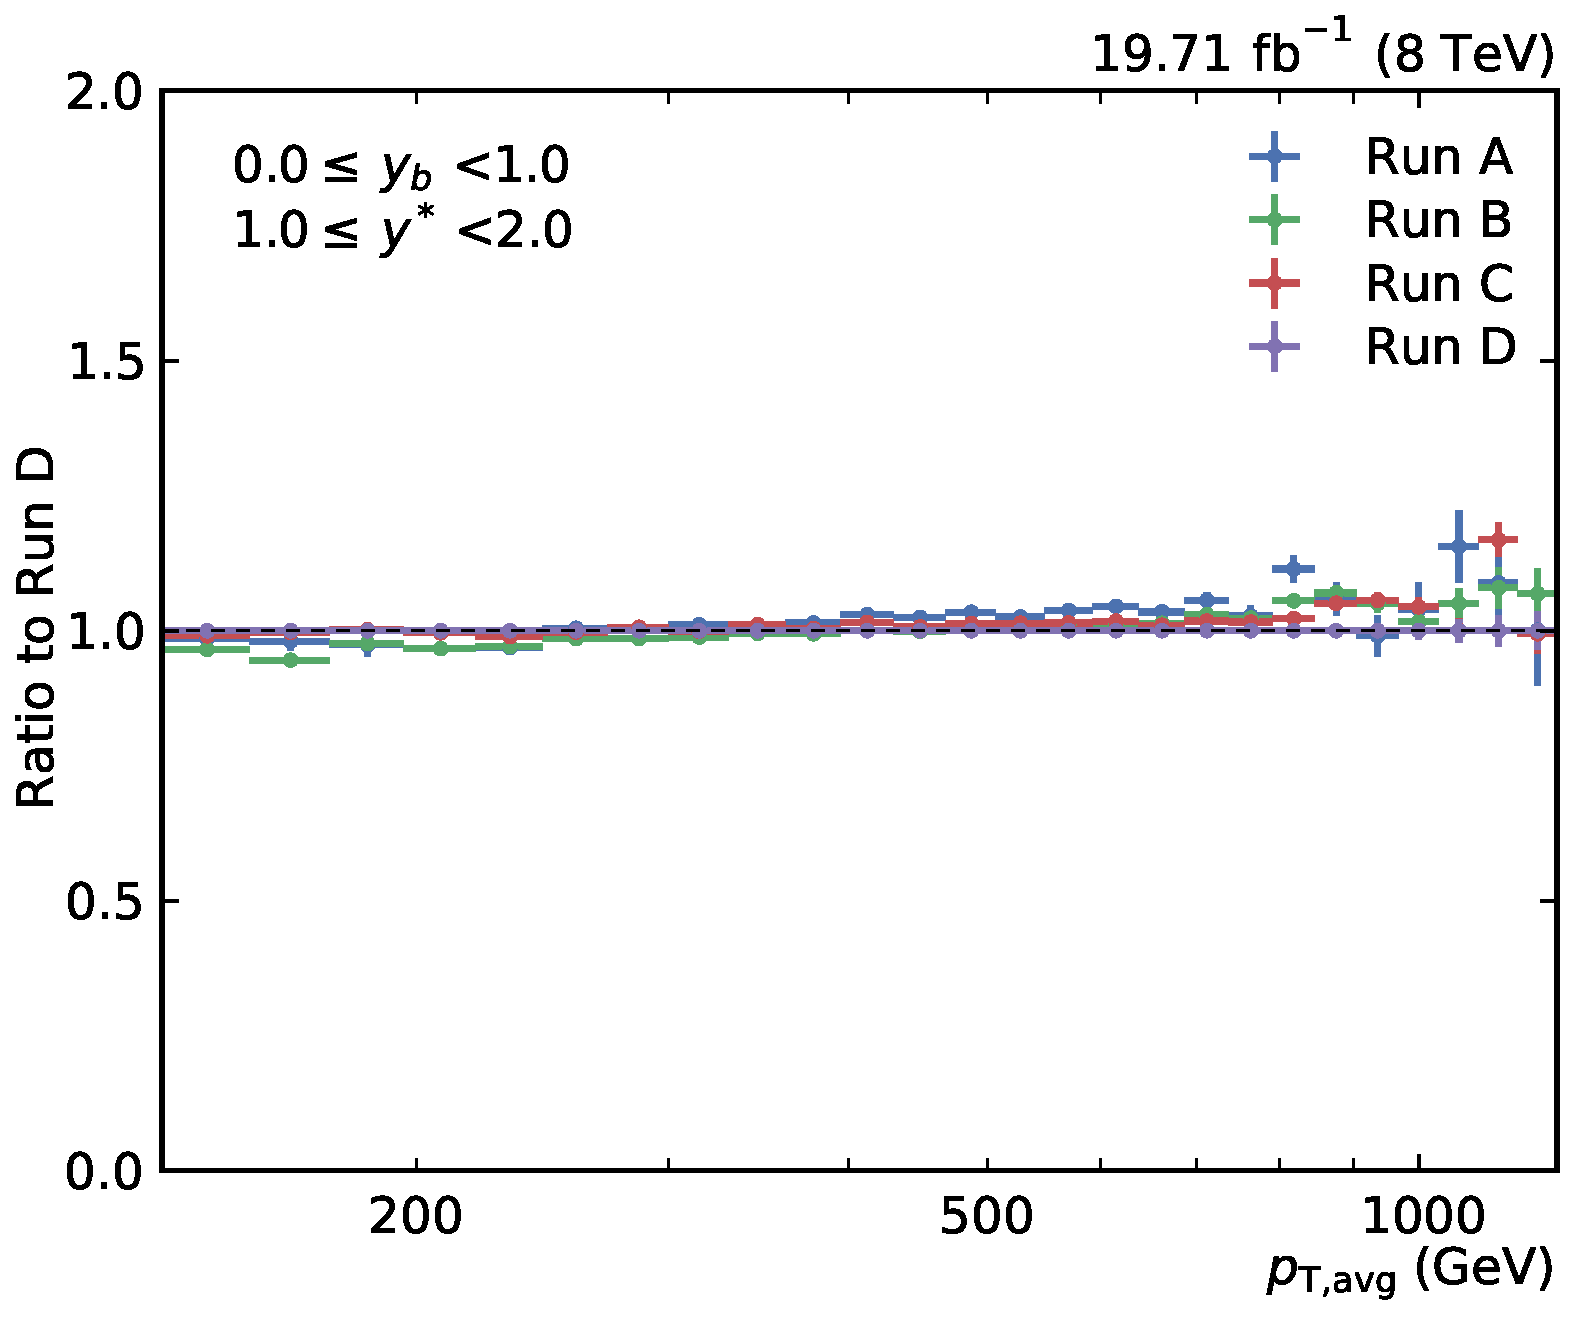
\includegraphics[width=0.47\textwidth]{figures/measurement/run_comparison_yb0ys1.pdf}
    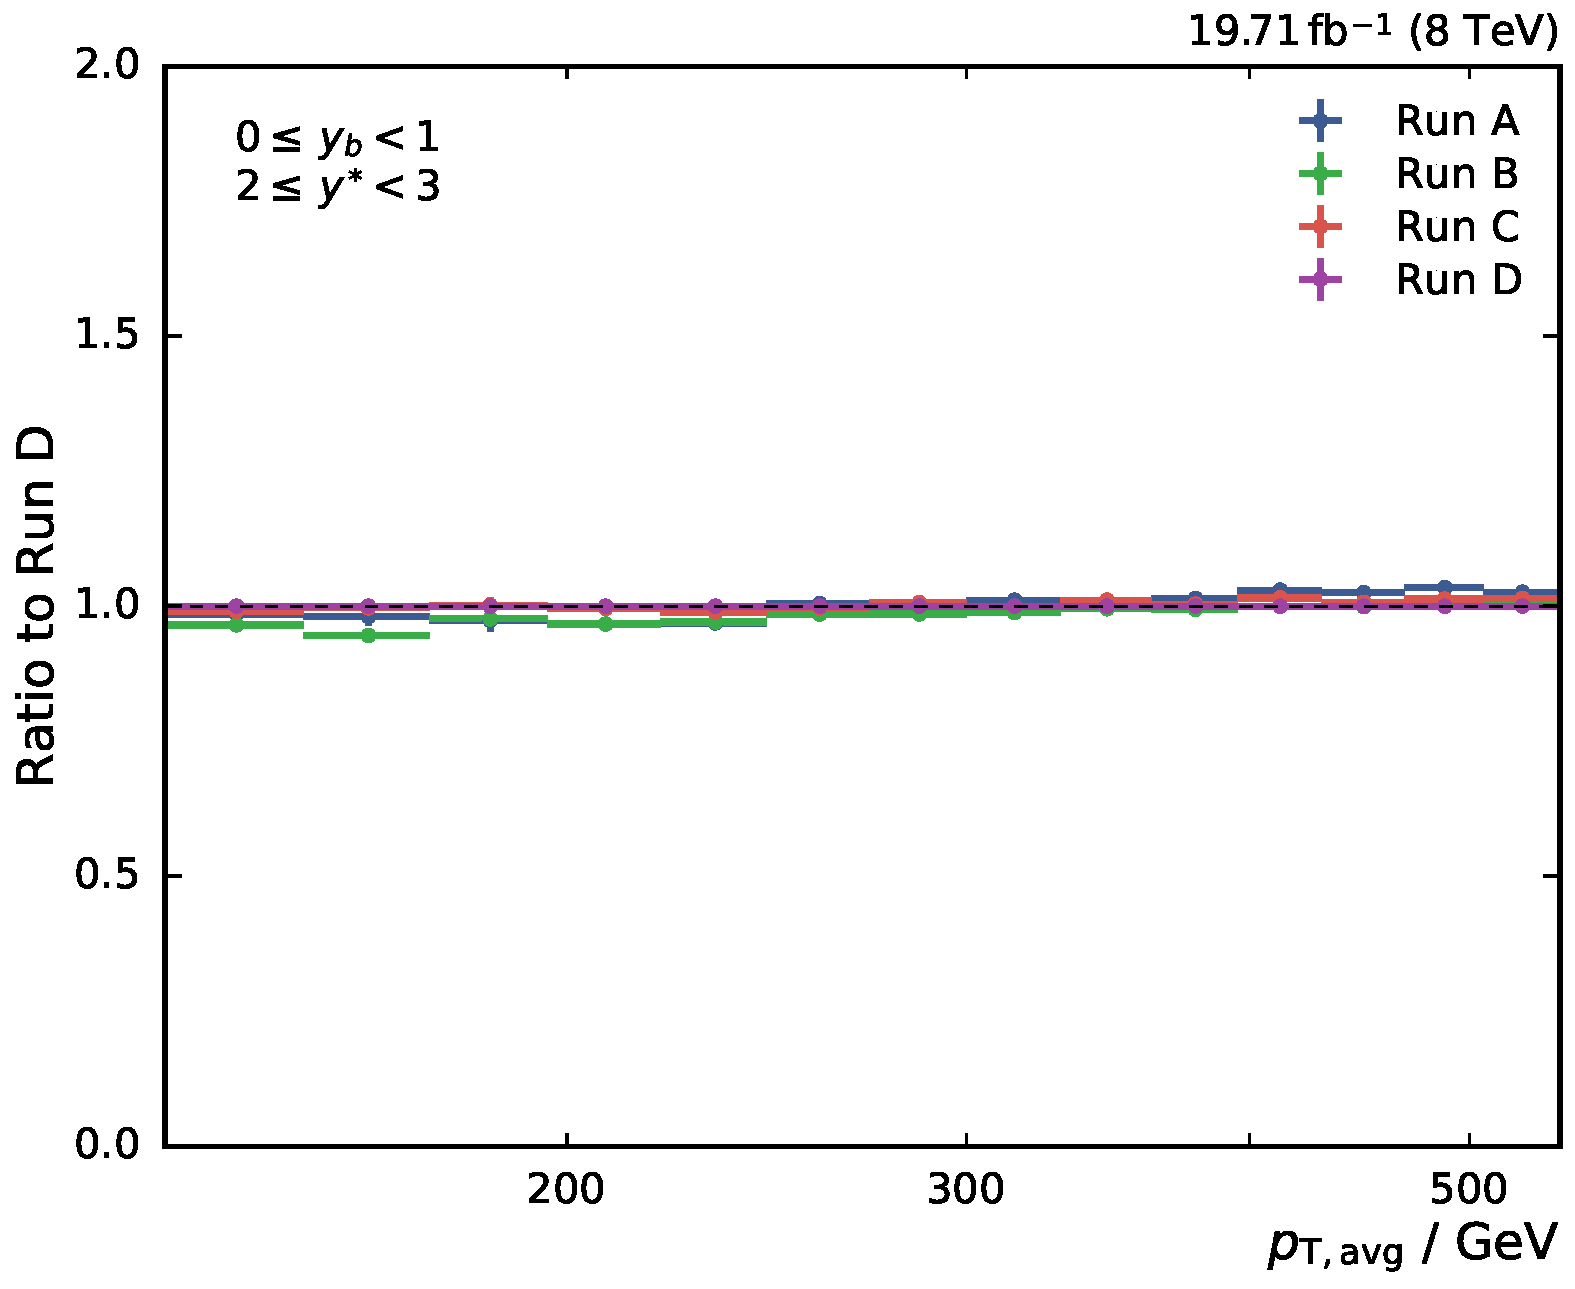
\includegraphics[width=0.47\textwidth]{figures/measurement/run_comparison_yb0ys2.pdf}\hfill
    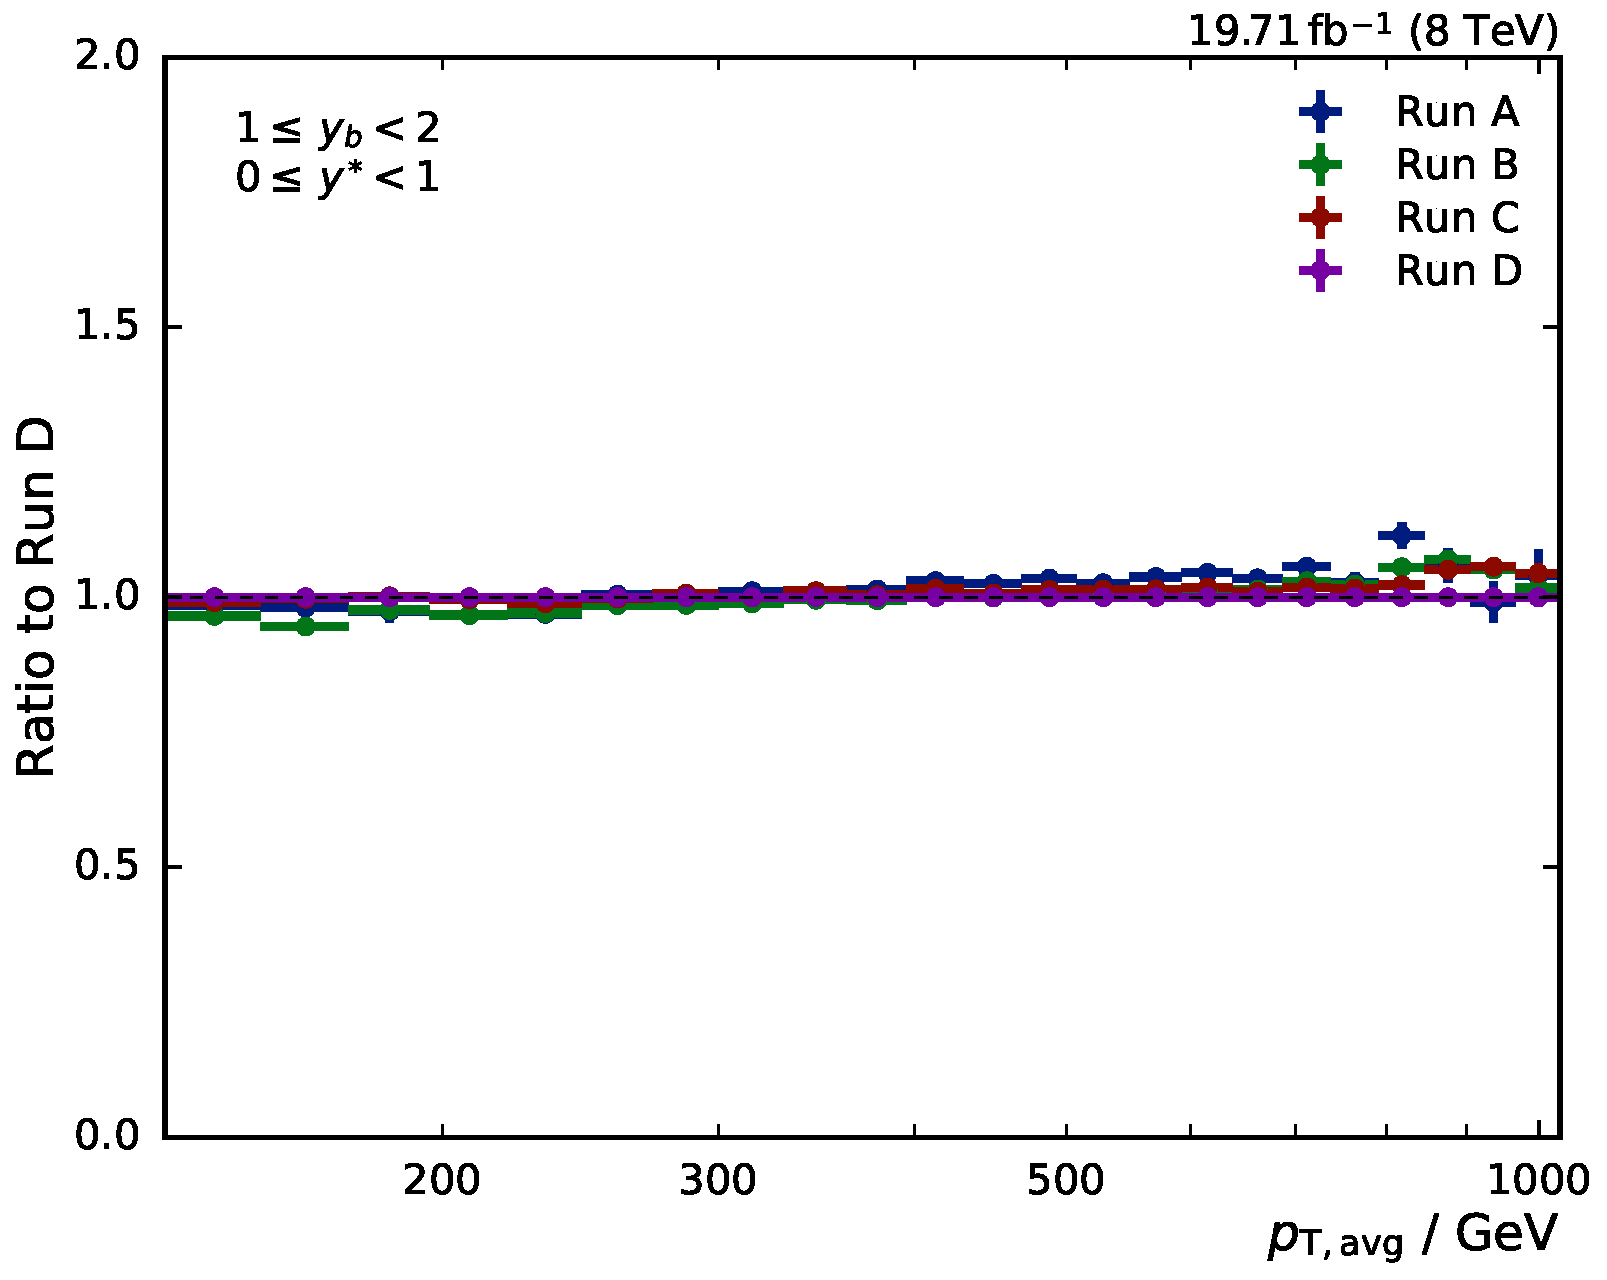
\includegraphics[width=0.47\textwidth]{figures/measurement/run_comparison_yb1ys0.pdf}
    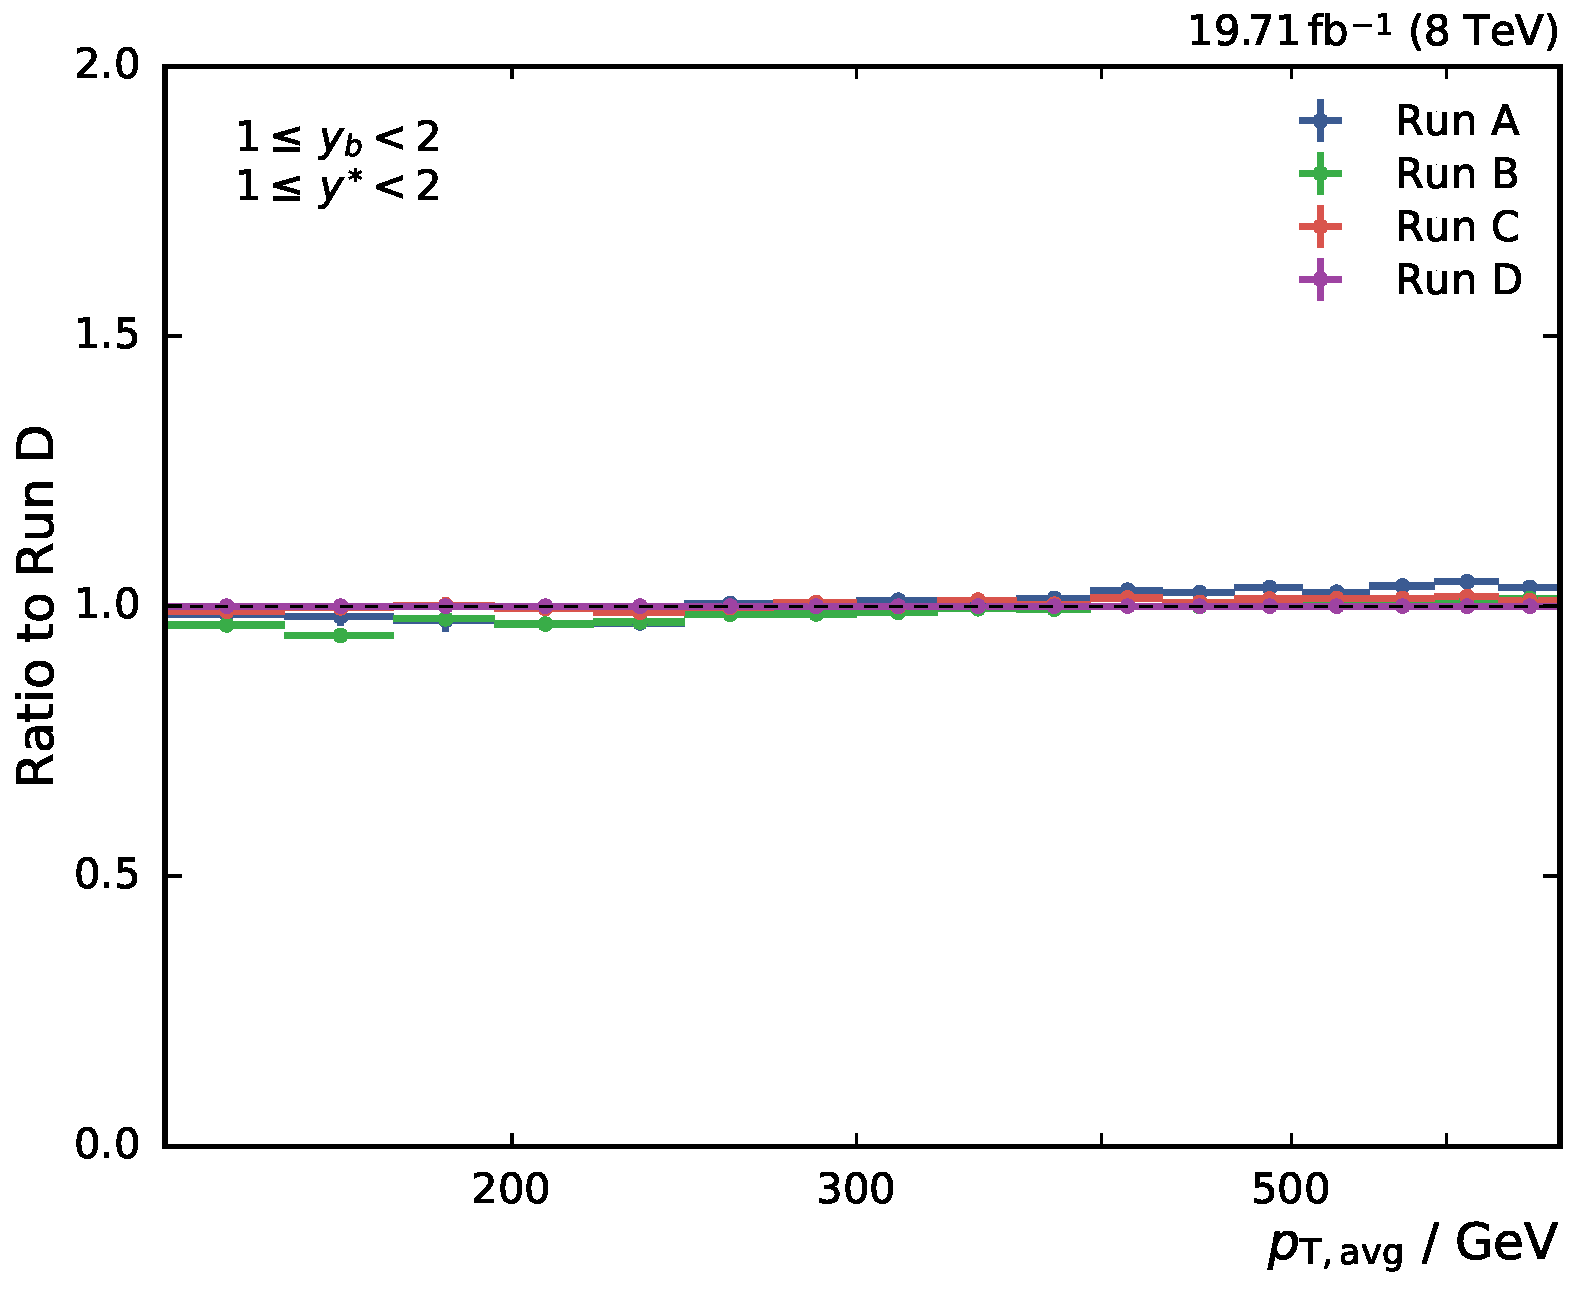
\includegraphics[width=0.47\textwidth]{figures/measurement/run_comparison_yb1ys1.pdf}\hfill
    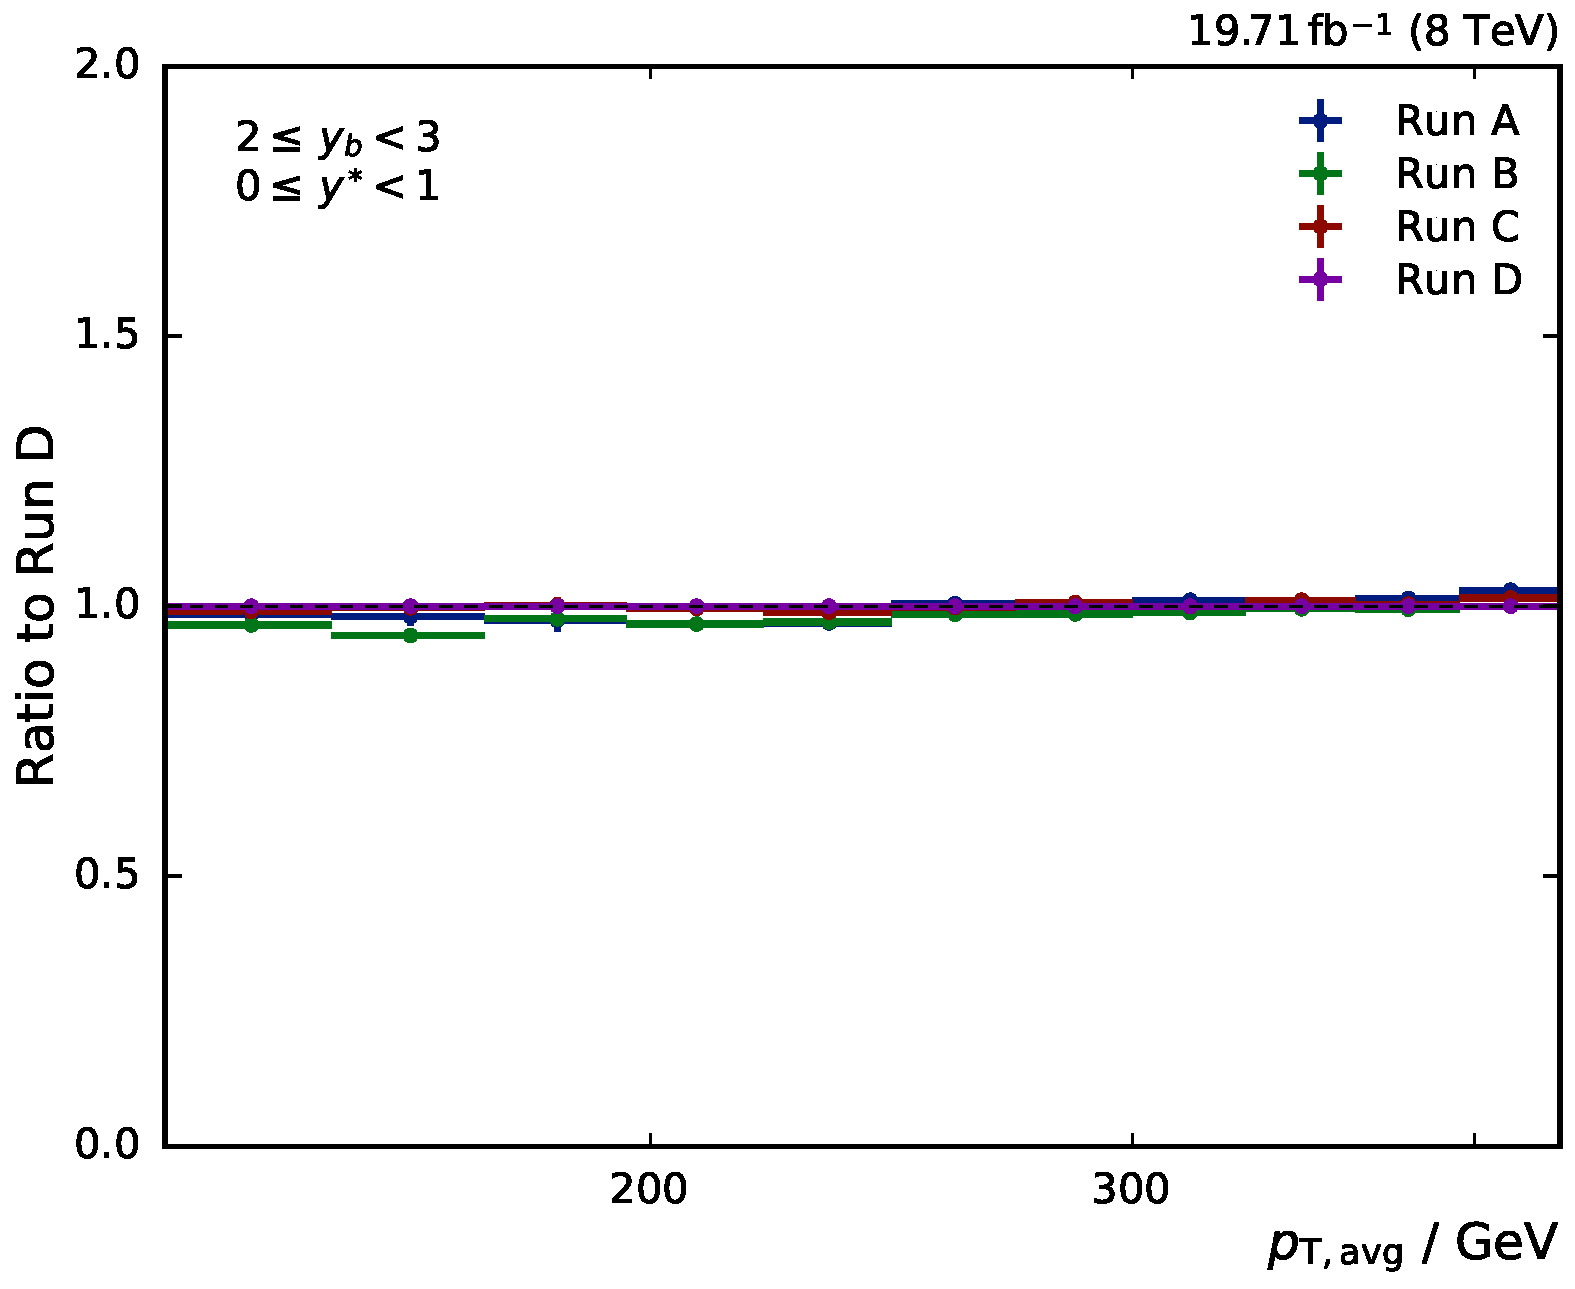
\includegraphics[width=0.47\textwidth]{figures/measurement/run_comparison_yb2ys0.pdf}
    \caption[Stability of result over all run periods]{Ratio of the measured
    cross section in each run period to the cross section obtained with data
    from run D. There are small differences, mostly due to statistical fluctuations.
    A slight slope is observed for the result of run B, but overall the separately
    obtained cross sections are in agreement within uncertainties.}
    \label{fig:run_comparison}
\end{figure}

\section{Comparison with Simulated Events}
\label{sec:simulated_events}

\subsection{Pileup Reweighting}

The official Monte Carlo samples are enriched with an admixture of pileup
collisions to mimic the pileup distribution expected in data. Ideally, the
estimated pileup distribution in data $N_\mathrm{data} (N_\mathrm{PU, est.})$
would match with the simulated distribution $N_\mathrm{MC} (N_\mathrm{PU,
truth})$. Since the admixture is only a rough estimate of the pileup
distribution expected in the forthcoming data taking, a perfect matching cannot
be achieved. To still get comparable pileup distributions in data and simulated
events, the simulated events are reweighted with $w_\mathrm{PU}$ to
match the distribution in data: 

\begin{equation*}
    w_{\mathrm{PU}} (N_{\mathrm{PU, truth}}) = \frac{N_\mathrm{data}
    (N_\mathrm{PU, est.}) / \sum N_\mathrm{data}}{N_\mathrm{MC}
    (N_\mathrm{PU, truth}) / \sum N_\mathrm{MC}}
\end{equation*}

Fig.~\ref{fig:mc:npv_reweighting} shows the number of reconstructed primary vertices
before and after reweighting. The significant mismatch of the
pileup distributions in data and simulated events, which can be observed before
reweighting the simulated events, has vanished.

\begin{figure}[htbp]
    \centering
    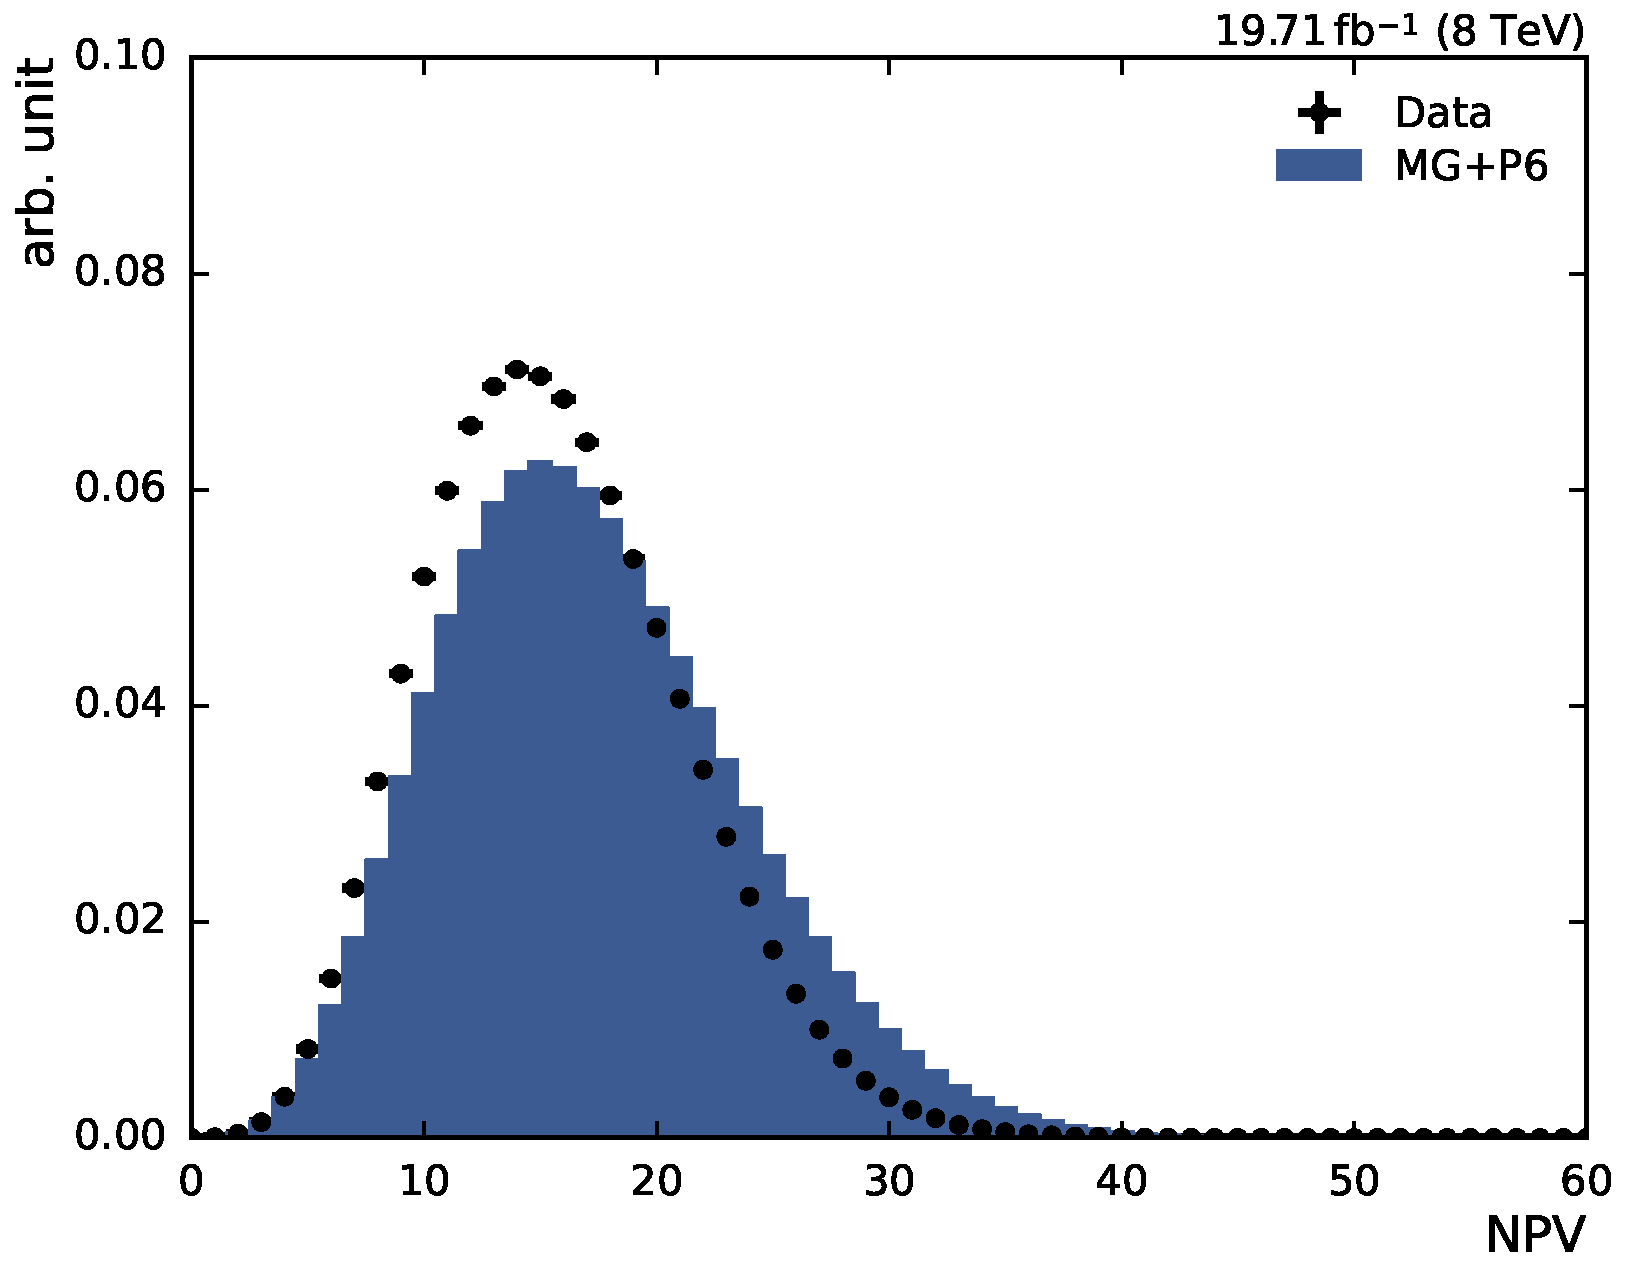
\includegraphics[width=0.47\textwidth]{figures/measurement/npv_beforereweighting.pdf}\hfill
    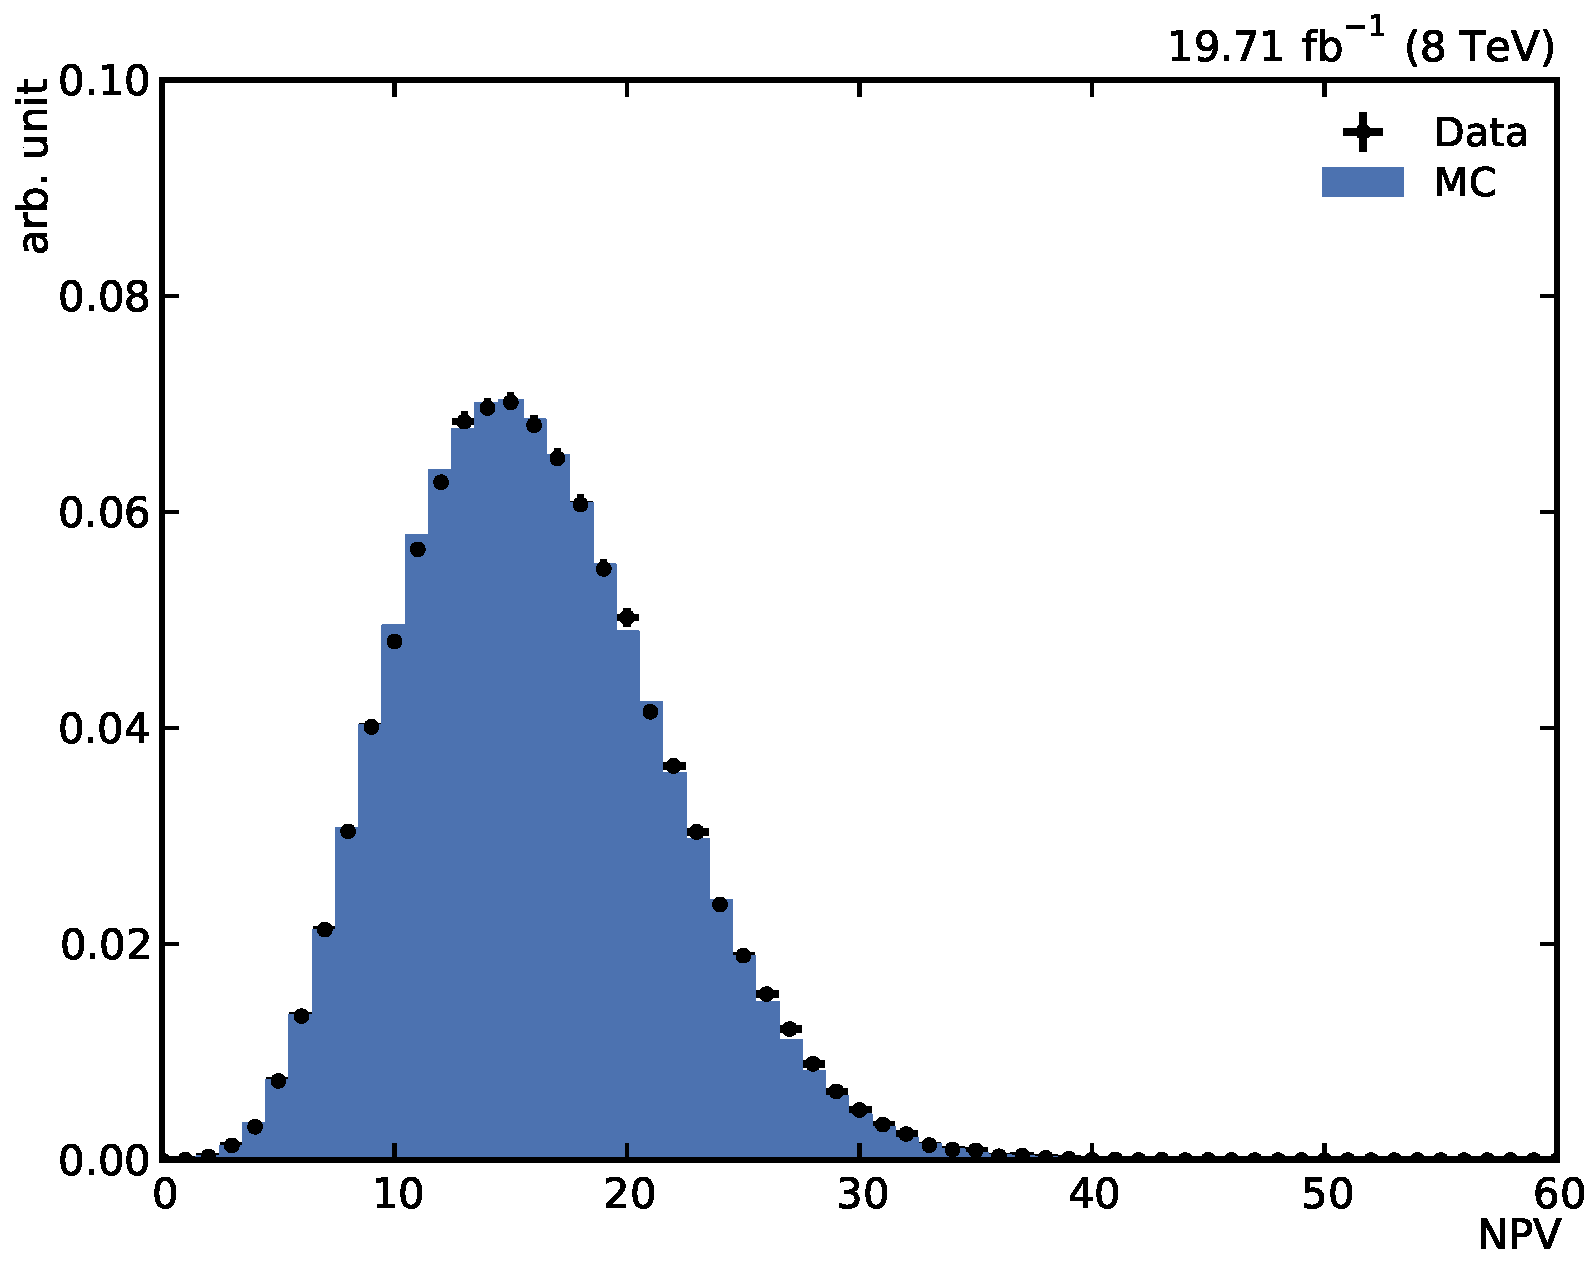
\includegraphics[width=0.47\textwidth]{figures/measurement/npv_afterreweighting.pdf}
    \caption[Number of reconstructed vertices]{Number of reconstructed vertices in data and simulated events before
    (left) and after (right) the pileup reweighting.}
    \label{fig:mc:npv_reweighting}
\end{figure}

\section{Kinematic Distributions}

The generated events are processed through the detector simulation and
reconstruction in order to compare kinematic quantities of dijet events with
simulated events on reconstructed level. Fig.~\ref{fig:controlplots:kinematic}
shows the transverse momentum $\pt$, the rapidity $y$ and the azimuthal angle
$\phi$ for the leading two jets. The \pt distribution is not that well described
especially in the low \pt region. While the rapidity distributions agree
within the tracker coverage of $|y| \leq 2.4$, there are larger
discrepancies at higher rapidities.

\begin{figure}[htbp]
    \centering
    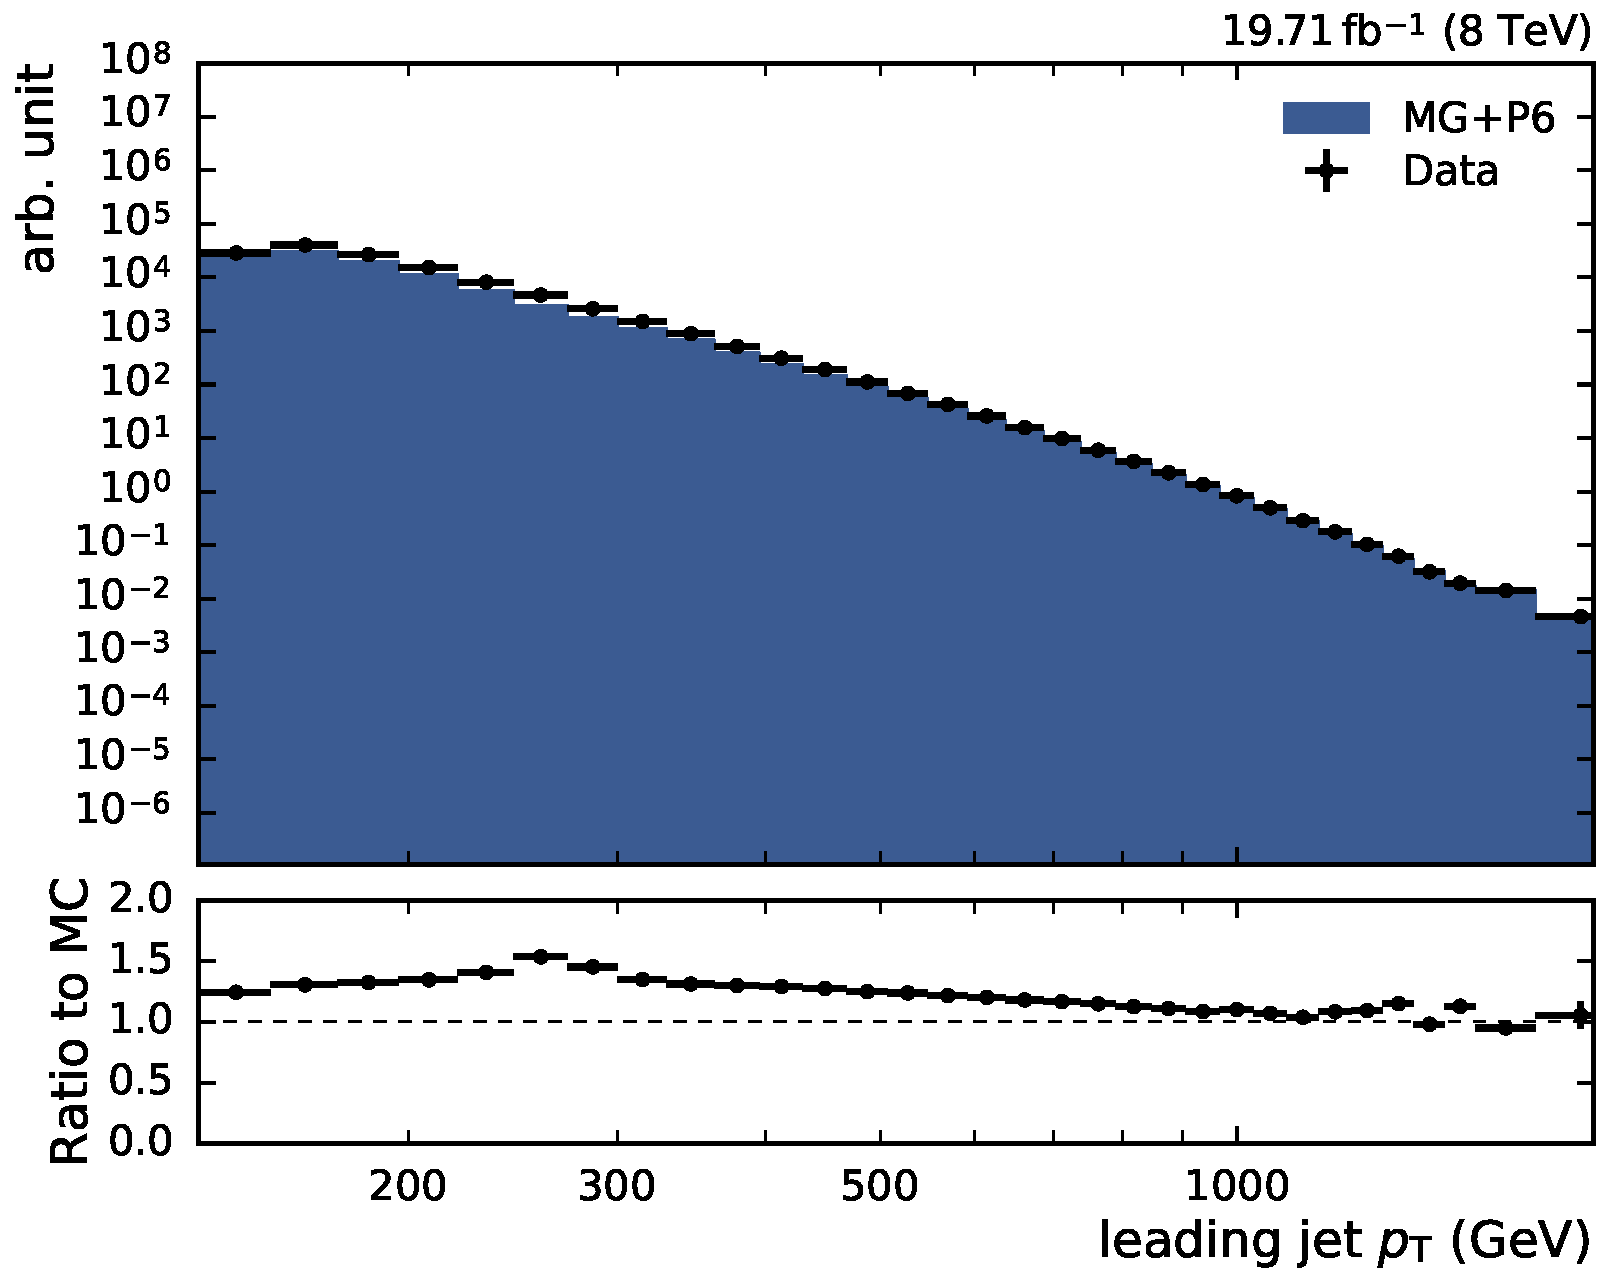
\includegraphics[width=0.47\textwidth]{figures/measurement/jet_quantities_jet1pt.pdf}\hfill
    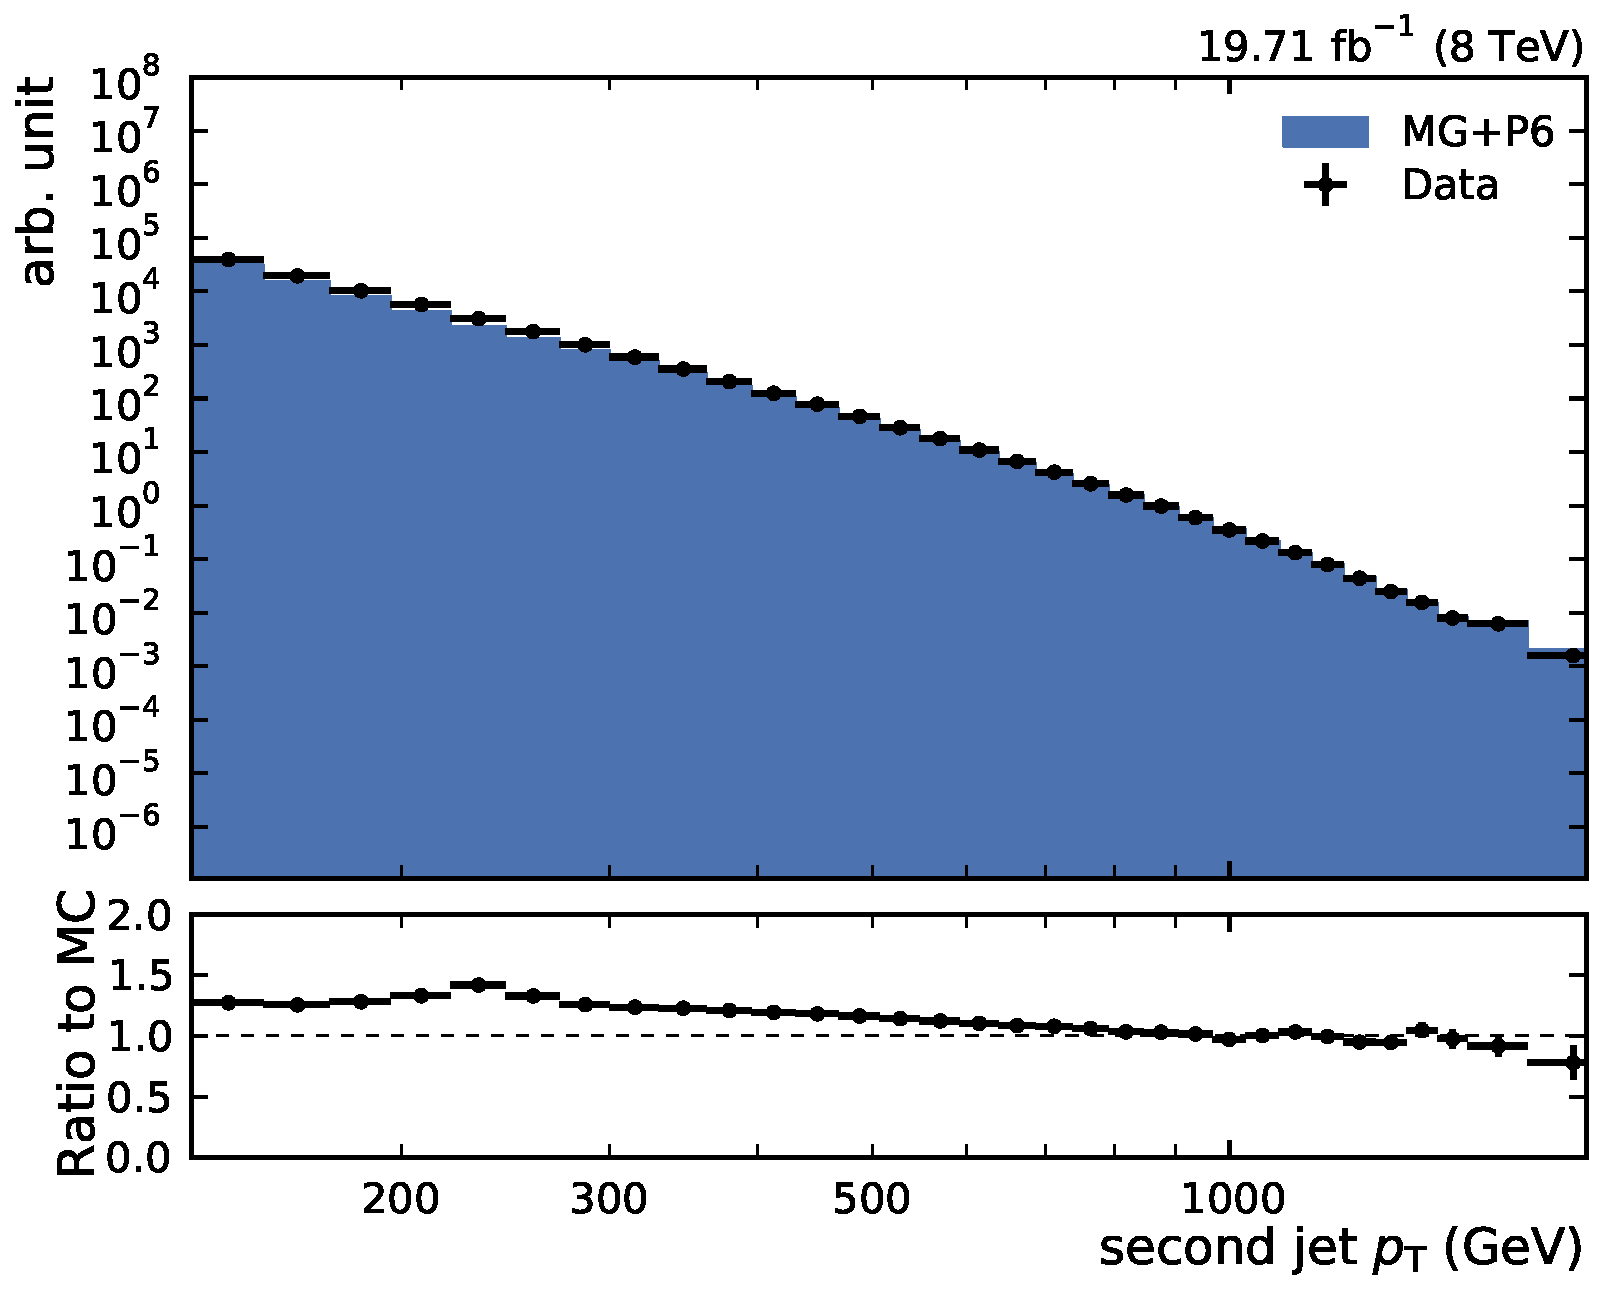
\includegraphics[width=0.47\textwidth]{figures/measurement/jet_quantities_jet2pt.pdf}
    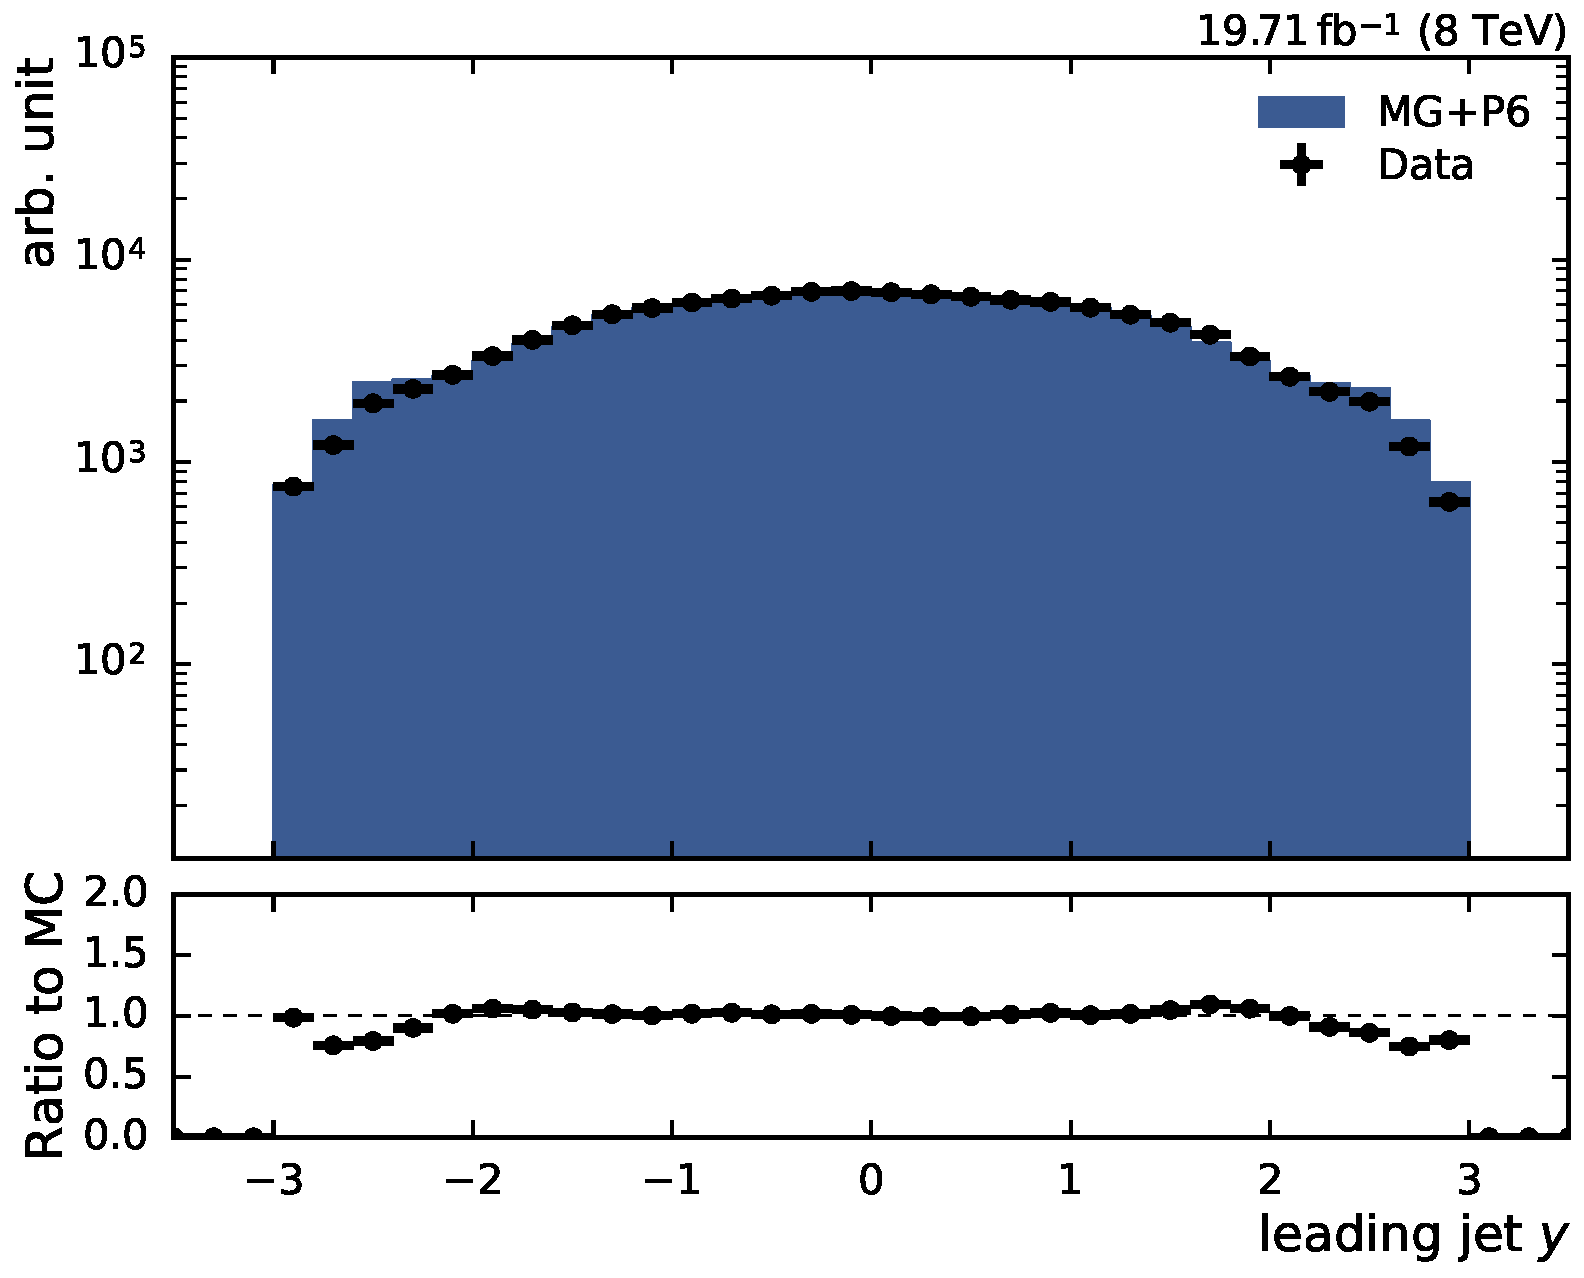
\includegraphics[width=0.47\textwidth]{figures/measurement/jet_quantities_jet1rap.pdf}\hfill
    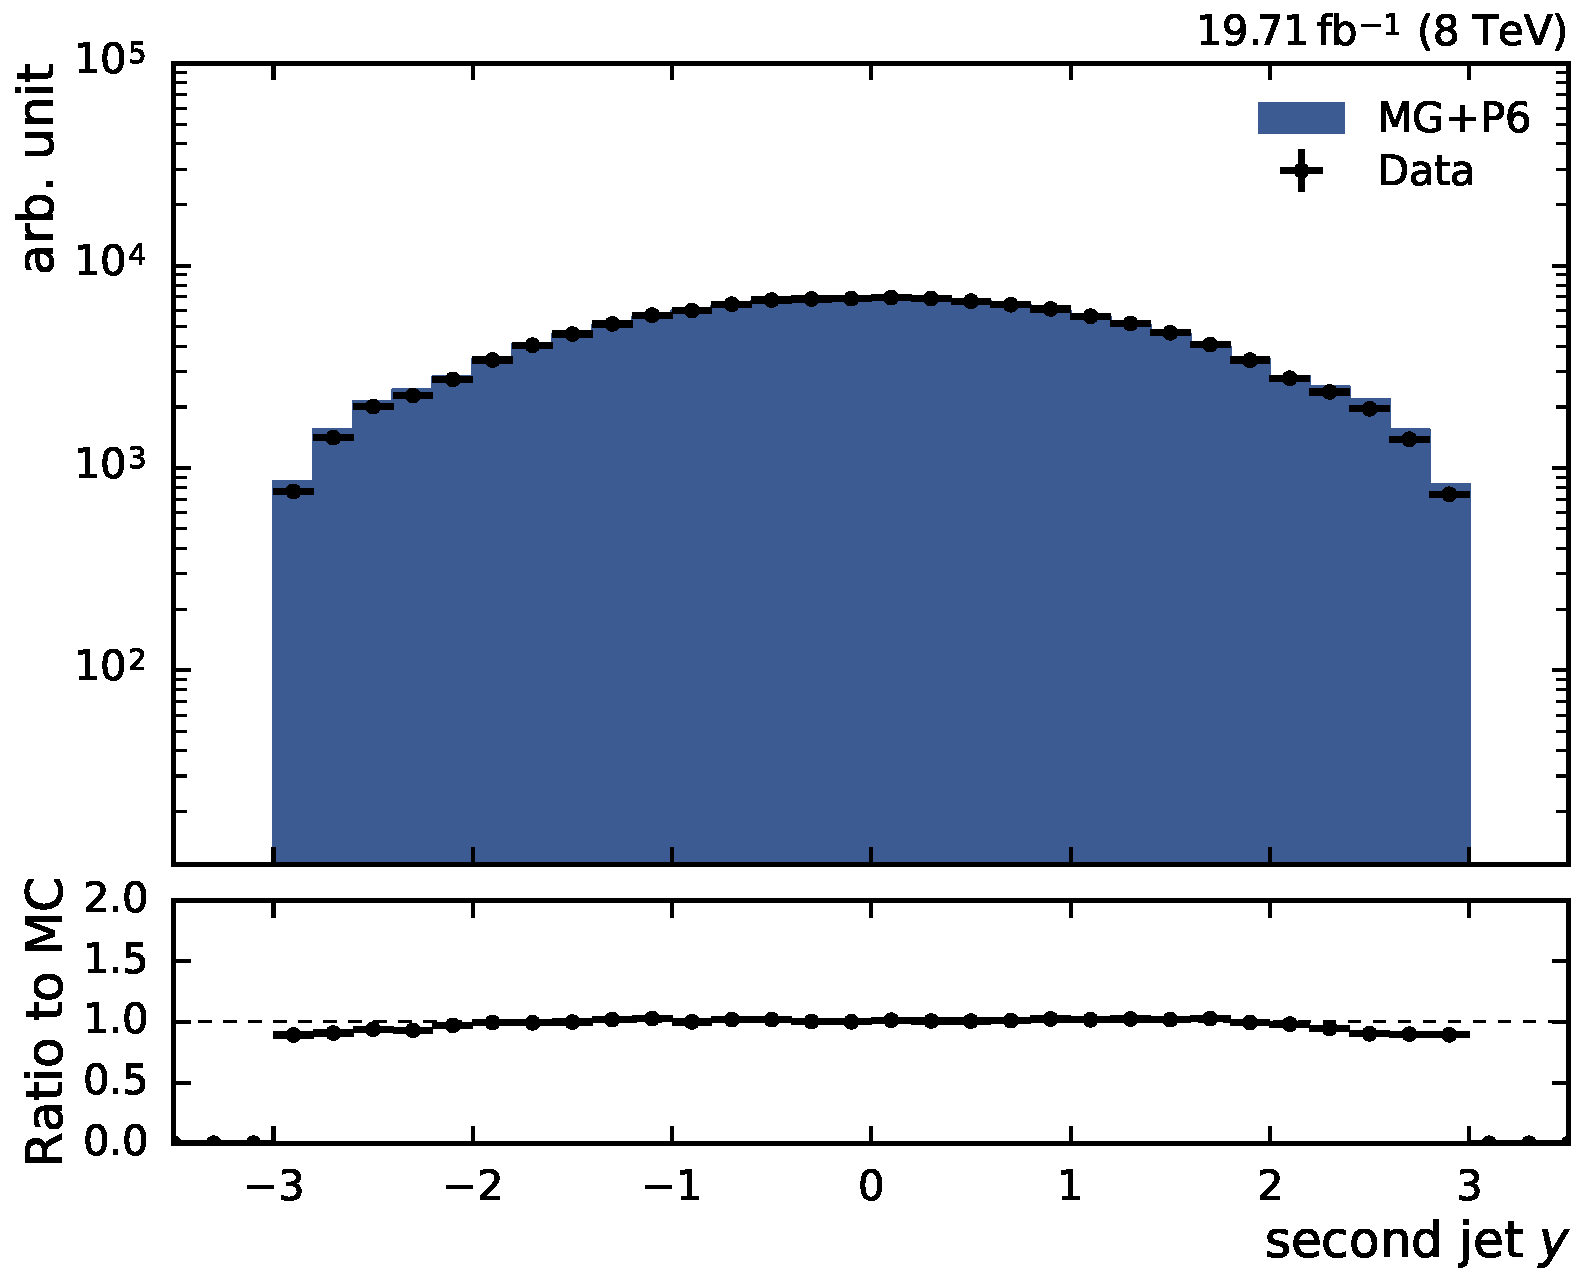
\includegraphics[width=0.47\textwidth]{figures/measurement/jet_quantities_jet2rap.pdf}
    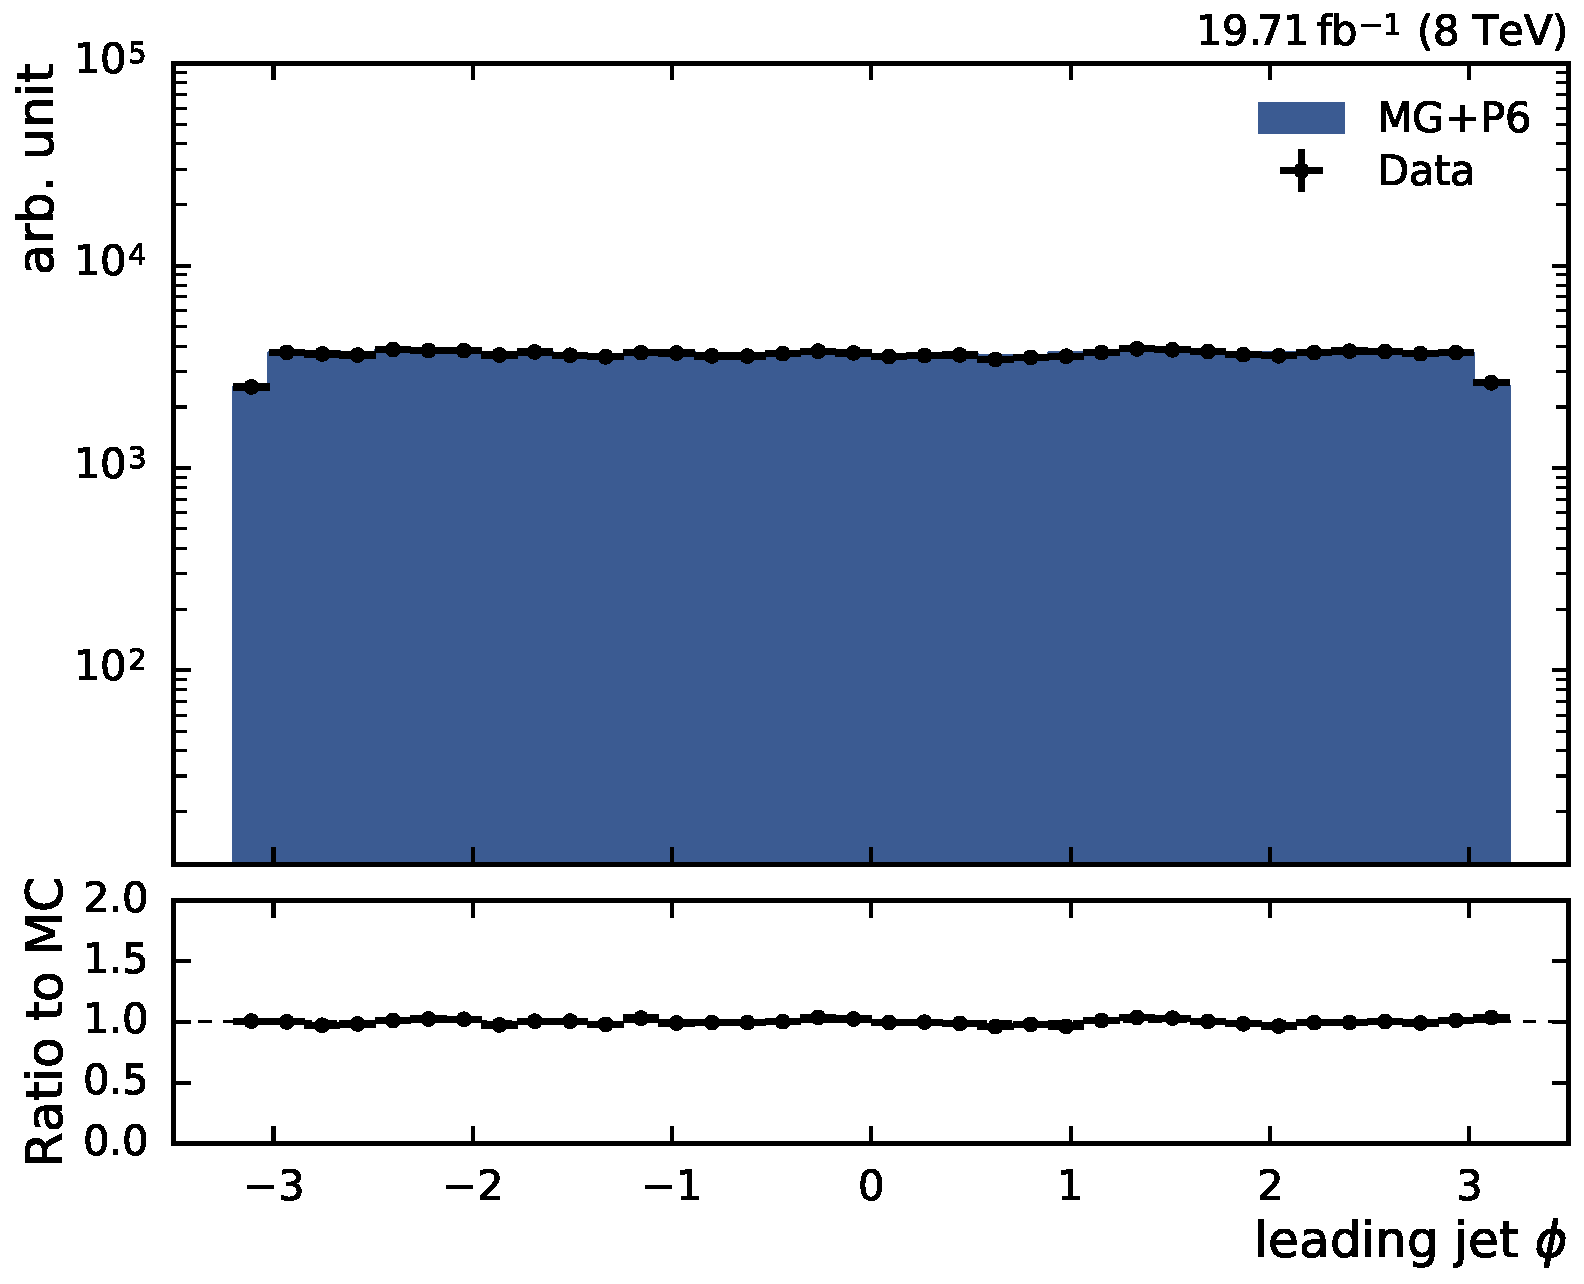
\includegraphics[width=0.47\textwidth]{figures/measurement/jet_quantities_jet1phi.pdf}\hfill
    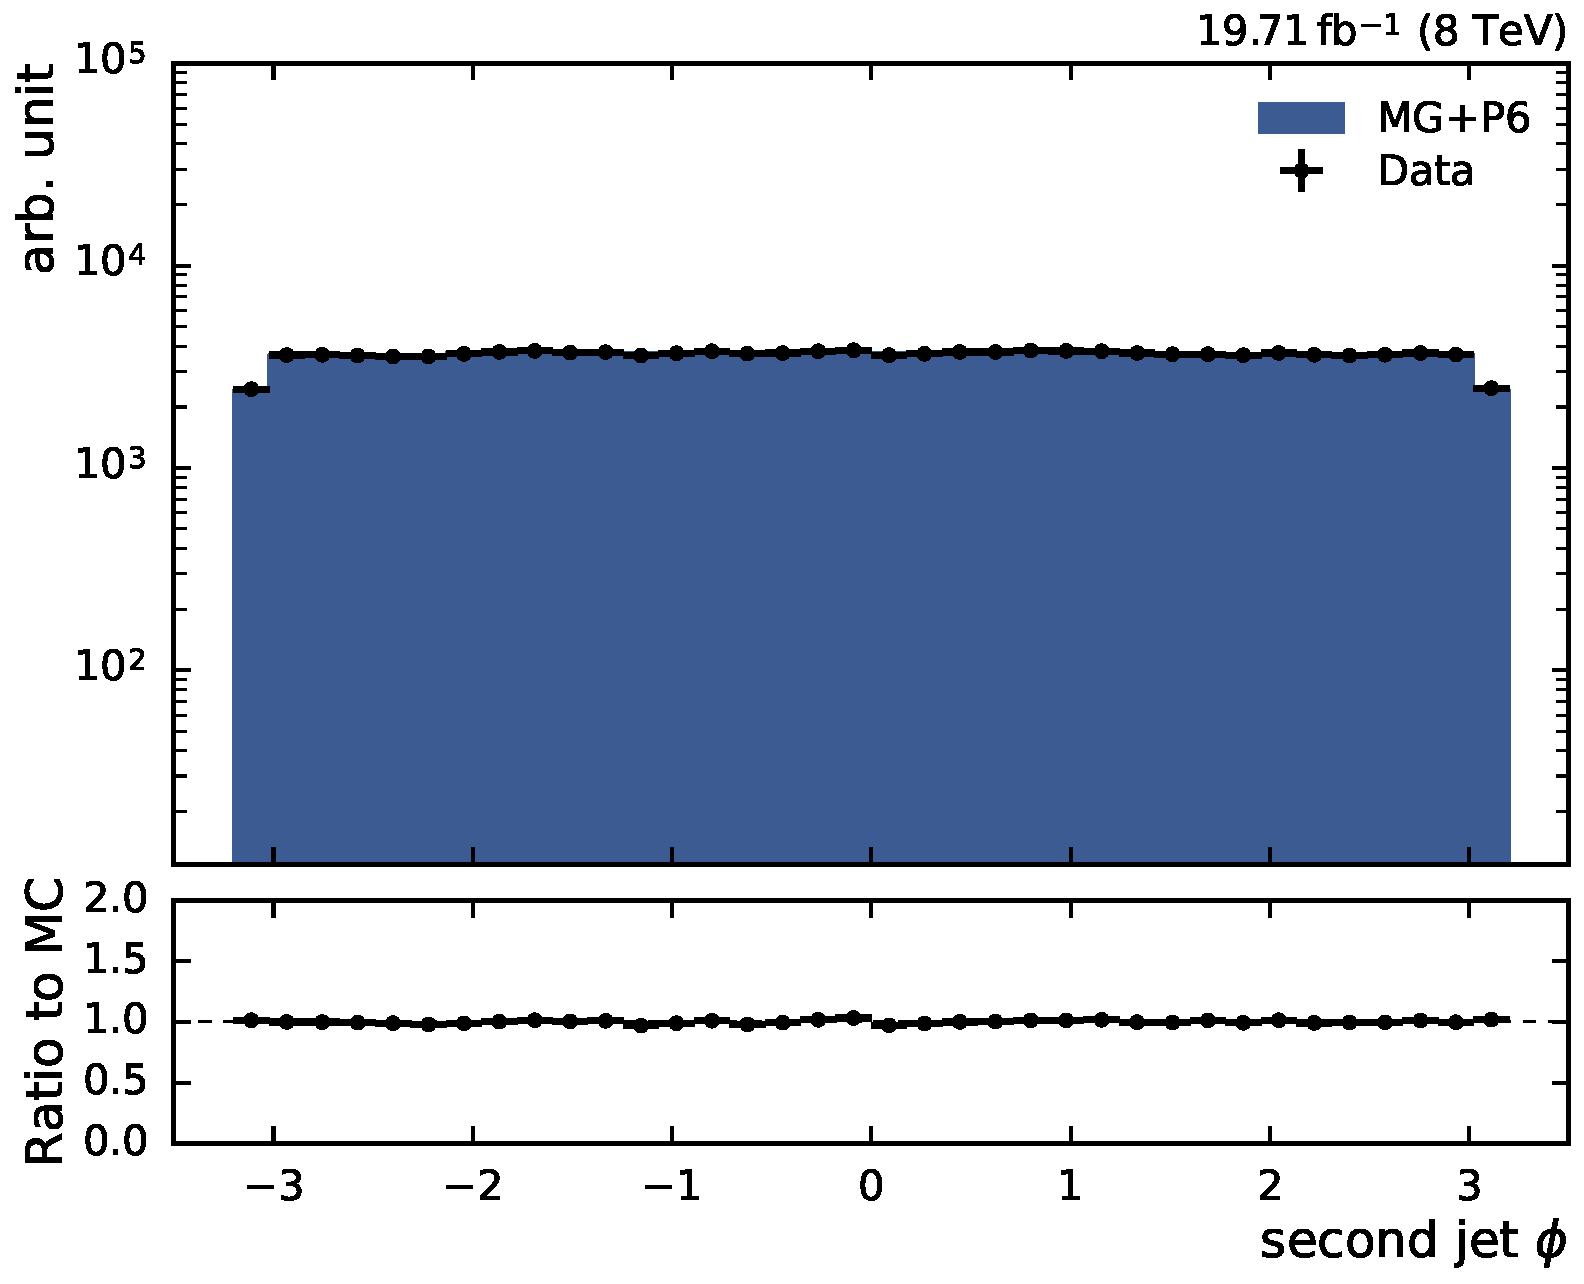
\includegraphics[width=0.47\textwidth]{figures/measurement/jet_quantities_jet2phi.pdf}
    \caption[Kinematic quantities of the jets]{Kinematic quantities are shown
        for the leading (left) and the subleading jet (right) both for data (markers) and
        simulated events (histogram). The rows show the transverse momentum
        (top), the rapidity (middle), and the azimuthal angle of the jets
    (bottom).}
    \label{fig:controlplots:kinematic}
\end{figure}

Kinematic distributions of the dijet system are shown in
Fig.~\ref{fig:controlplots:dijets}. The azimuthal difference $\Delta\phi$ and
the distance $\Delta R$ in the $\eta$-$\phi$ plane is well described by the
simulated events. The dijet mass $M_{1,2}$ and the average \pt of the dijet
system are in agreement only at lower transverse momentum. At high dijet
masses and transverse momenta, the theory significantly overestimates the data.
The shape of the boost and rapidity separation distributions is well described
for central jets. For very forward jets which are outside the coverage of the
tracker, a significant difference is observed.

\begin{figure}[htbp]
    \centering
    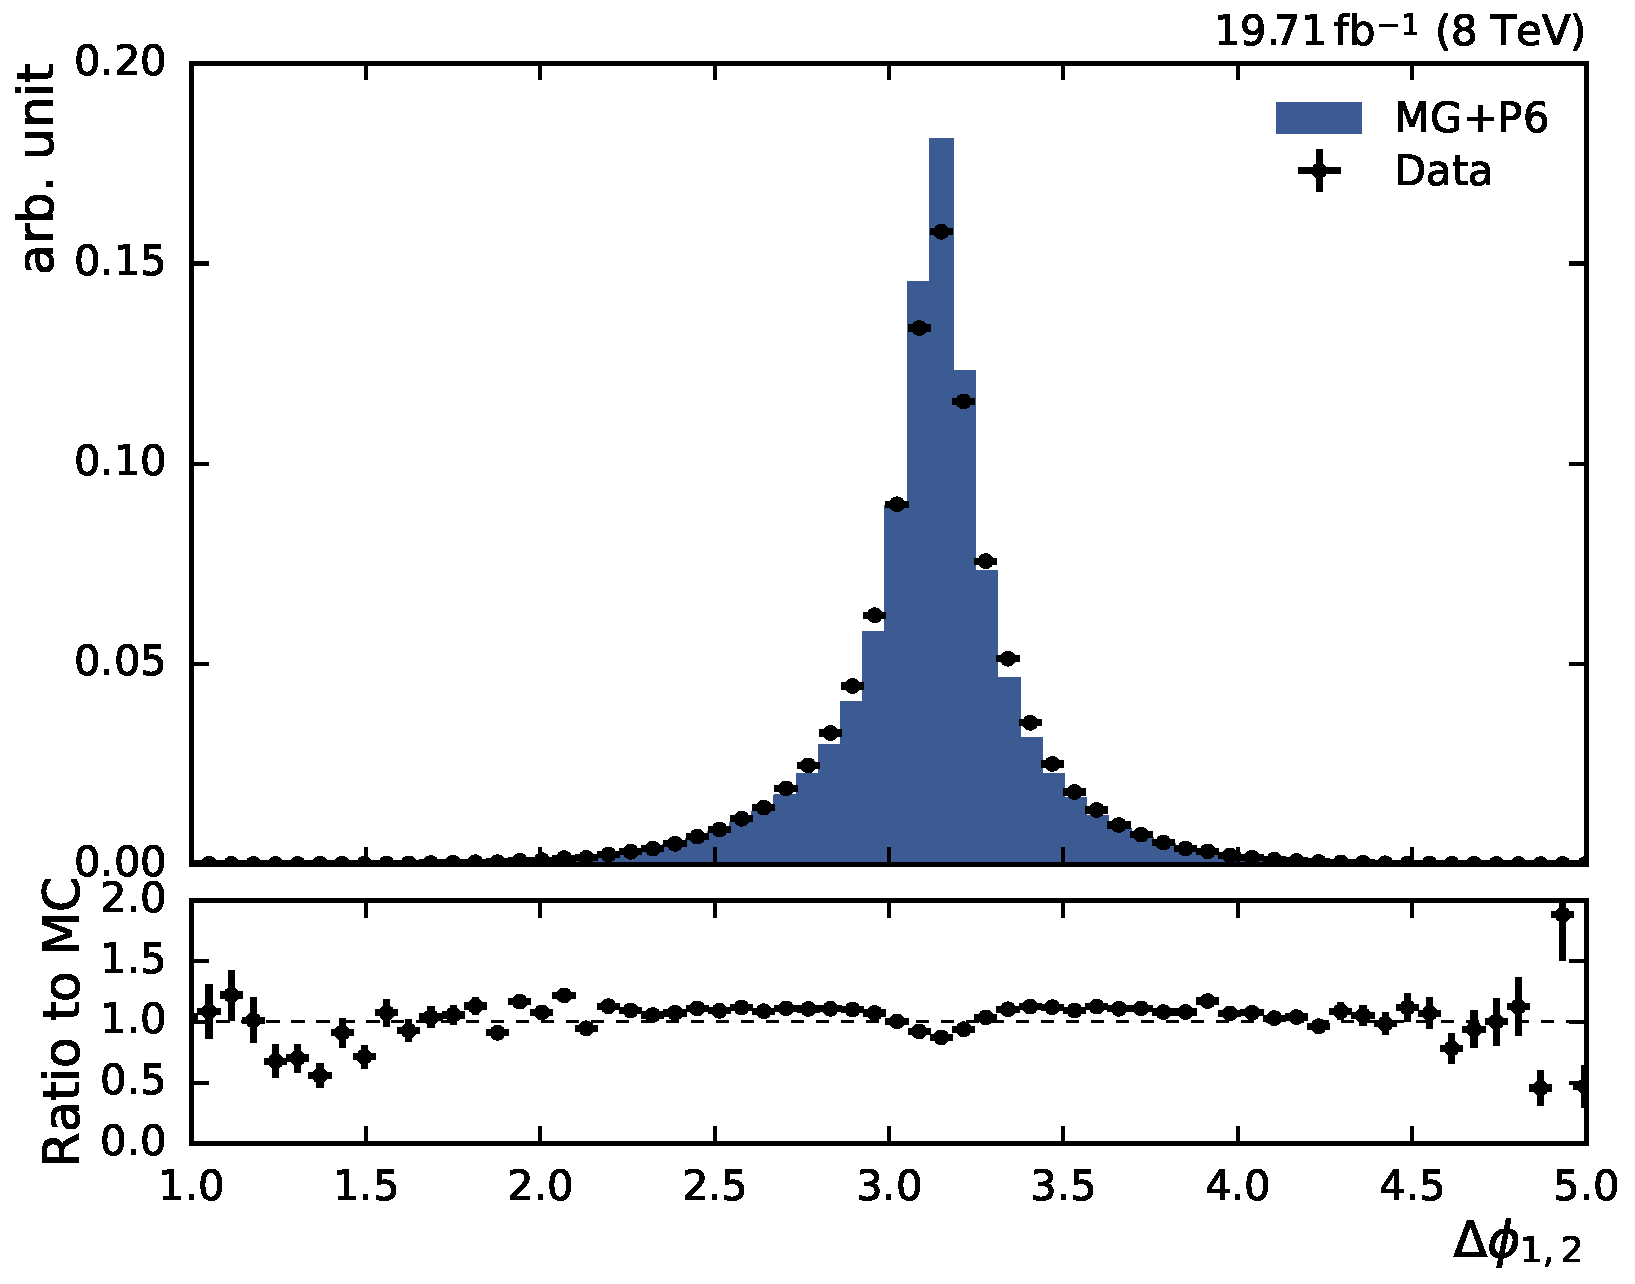
\includegraphics[width=0.47\textwidth]{figures/measurement/dijet_quantities_dijet_deltaphi.pdf}\hfill
    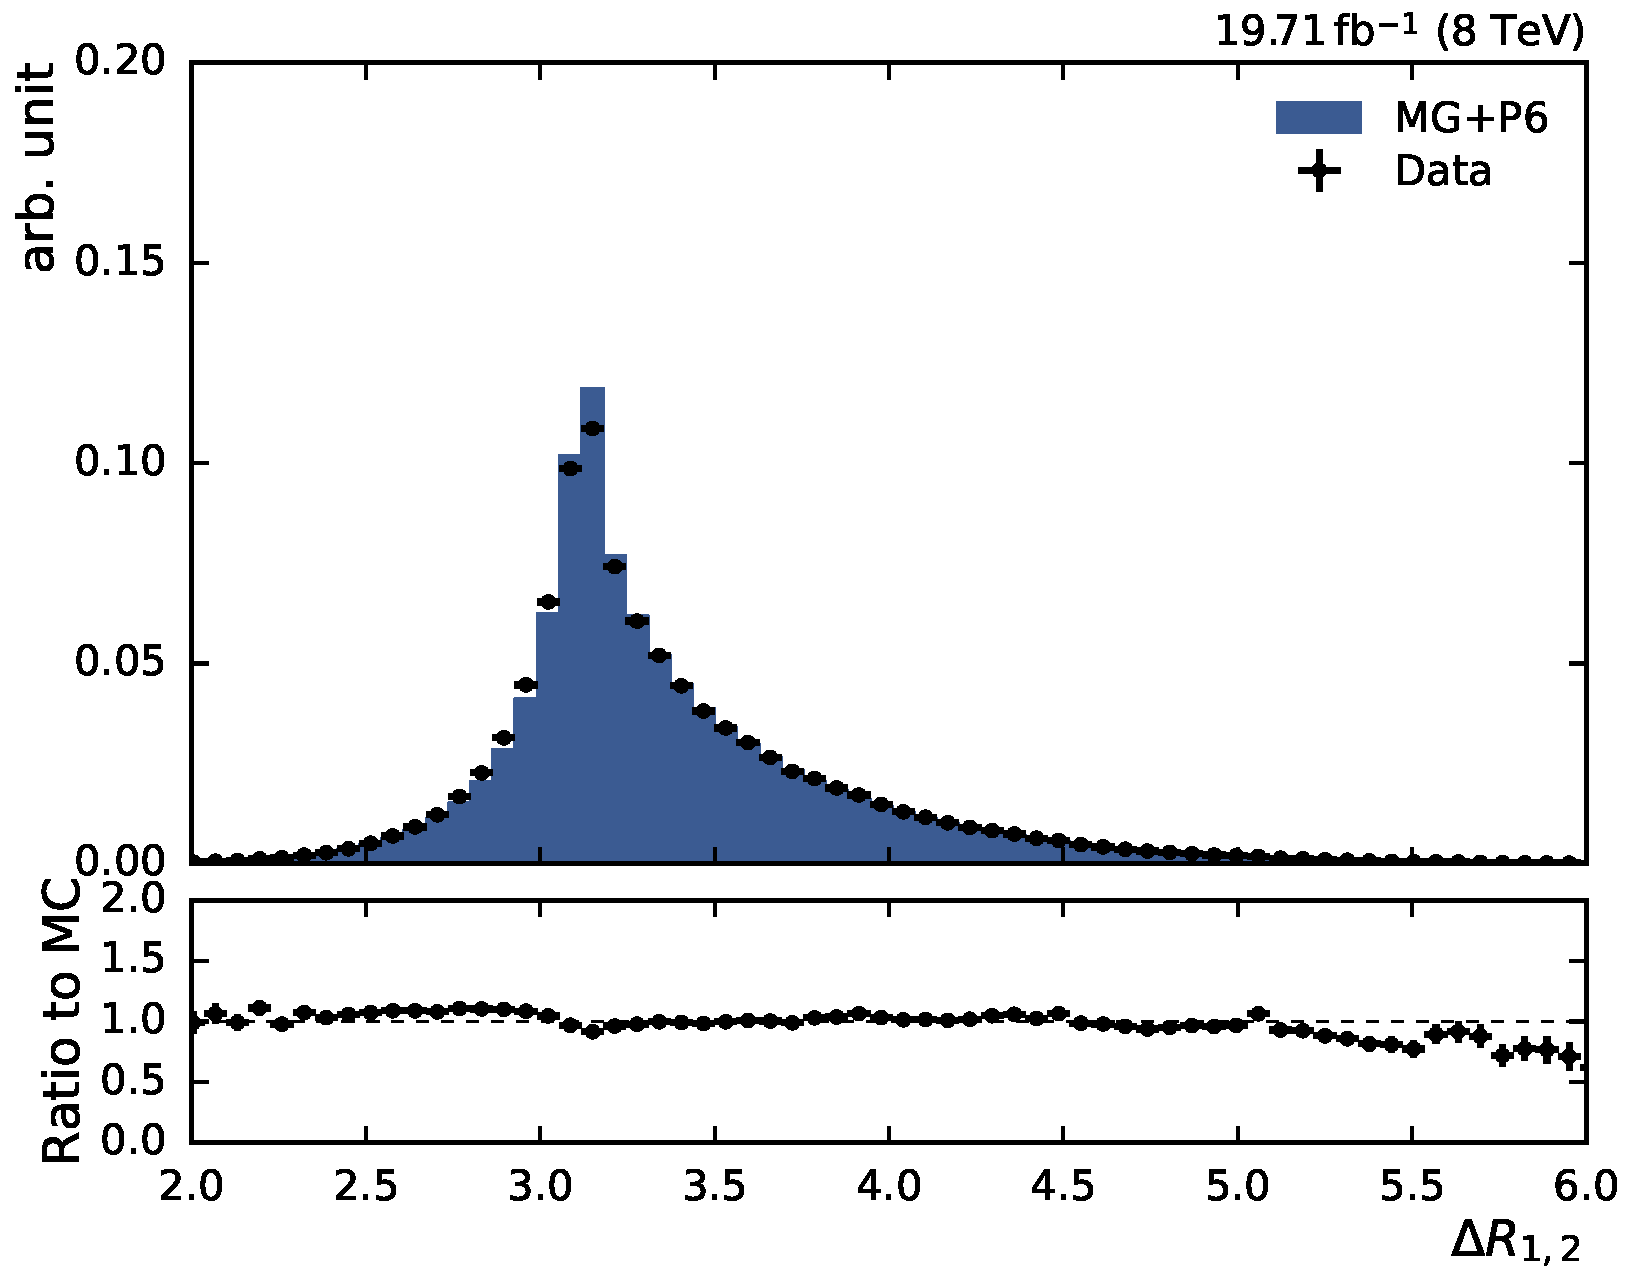
\includegraphics[width=0.47\textwidth]{figures/measurement/dijet_quantities_dijet_deltar.pdf}
    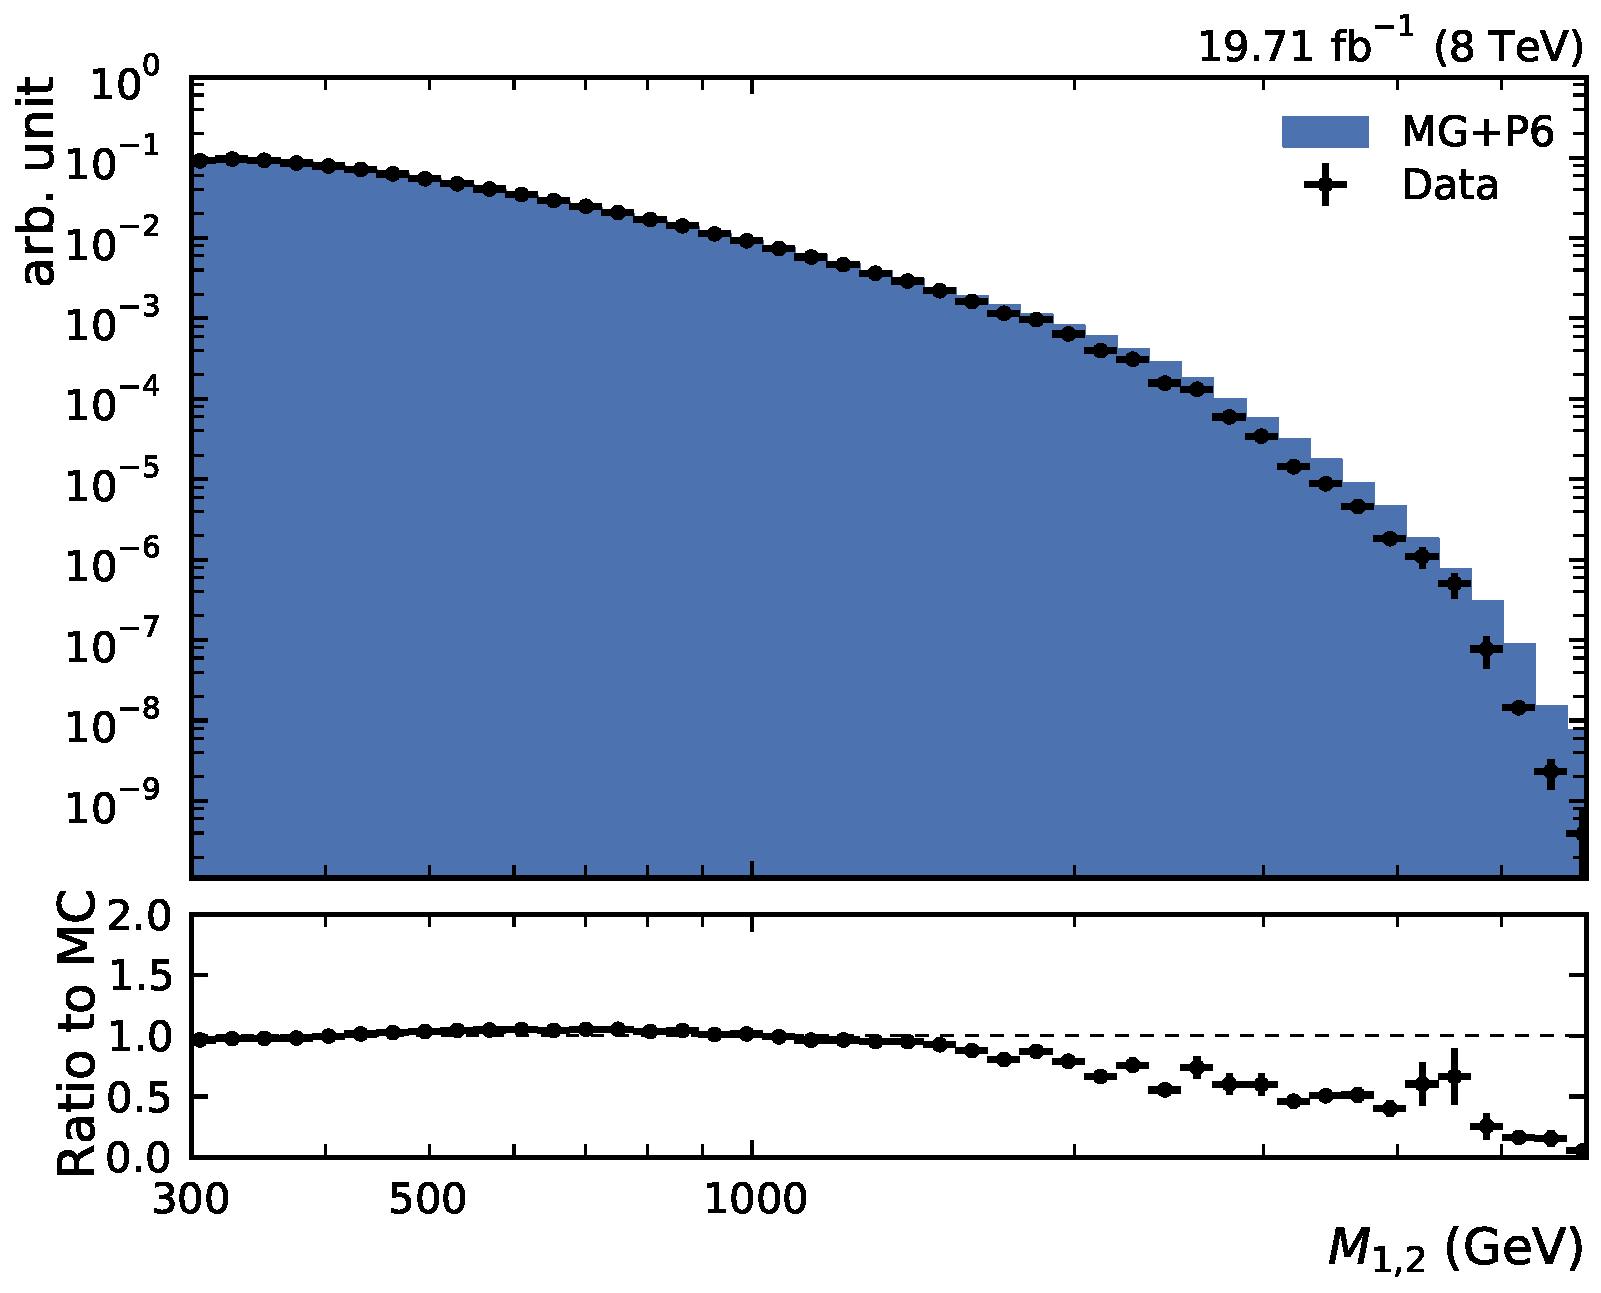
\includegraphics[width=0.47\textwidth]{figures/measurement/dijet_quantities_dijet_mass.pdf}\hfill
    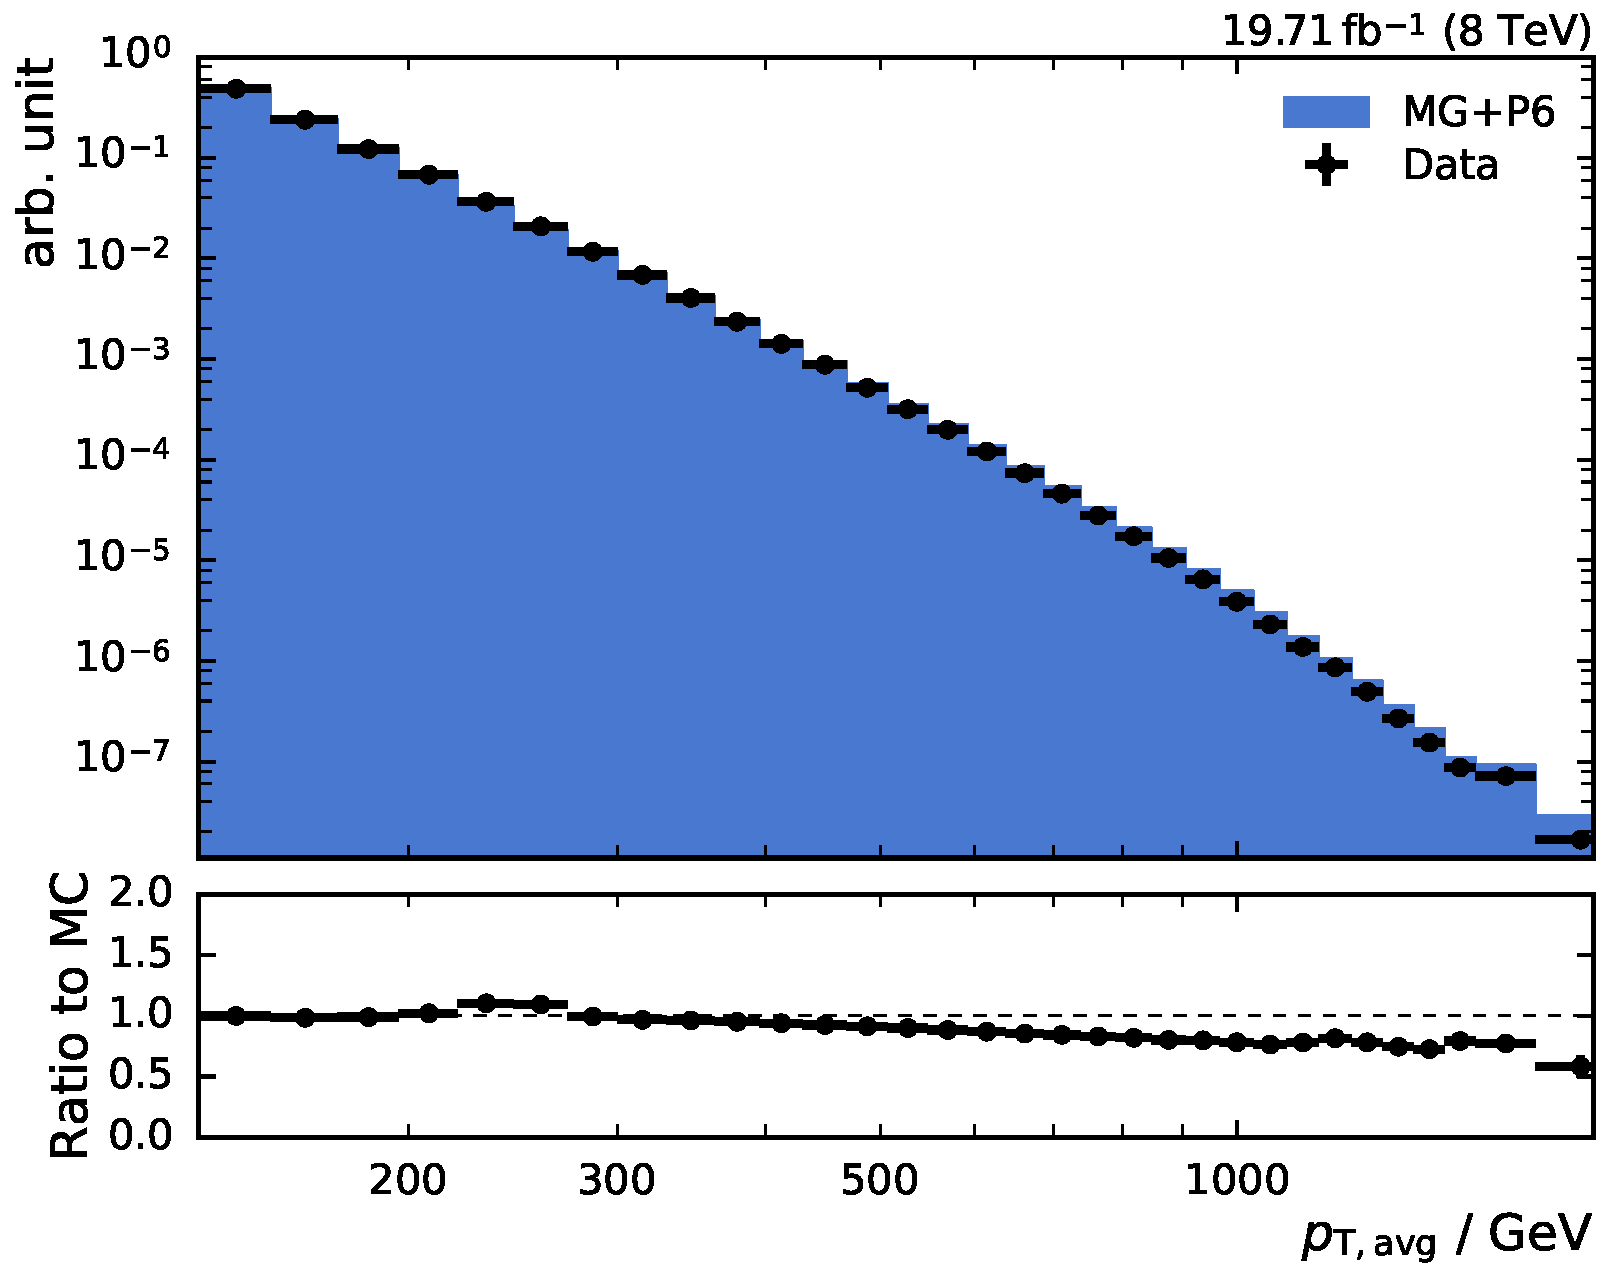
\includegraphics[width=0.47\textwidth]{figures/measurement/dijet_quantities_ptavg.pdf}
    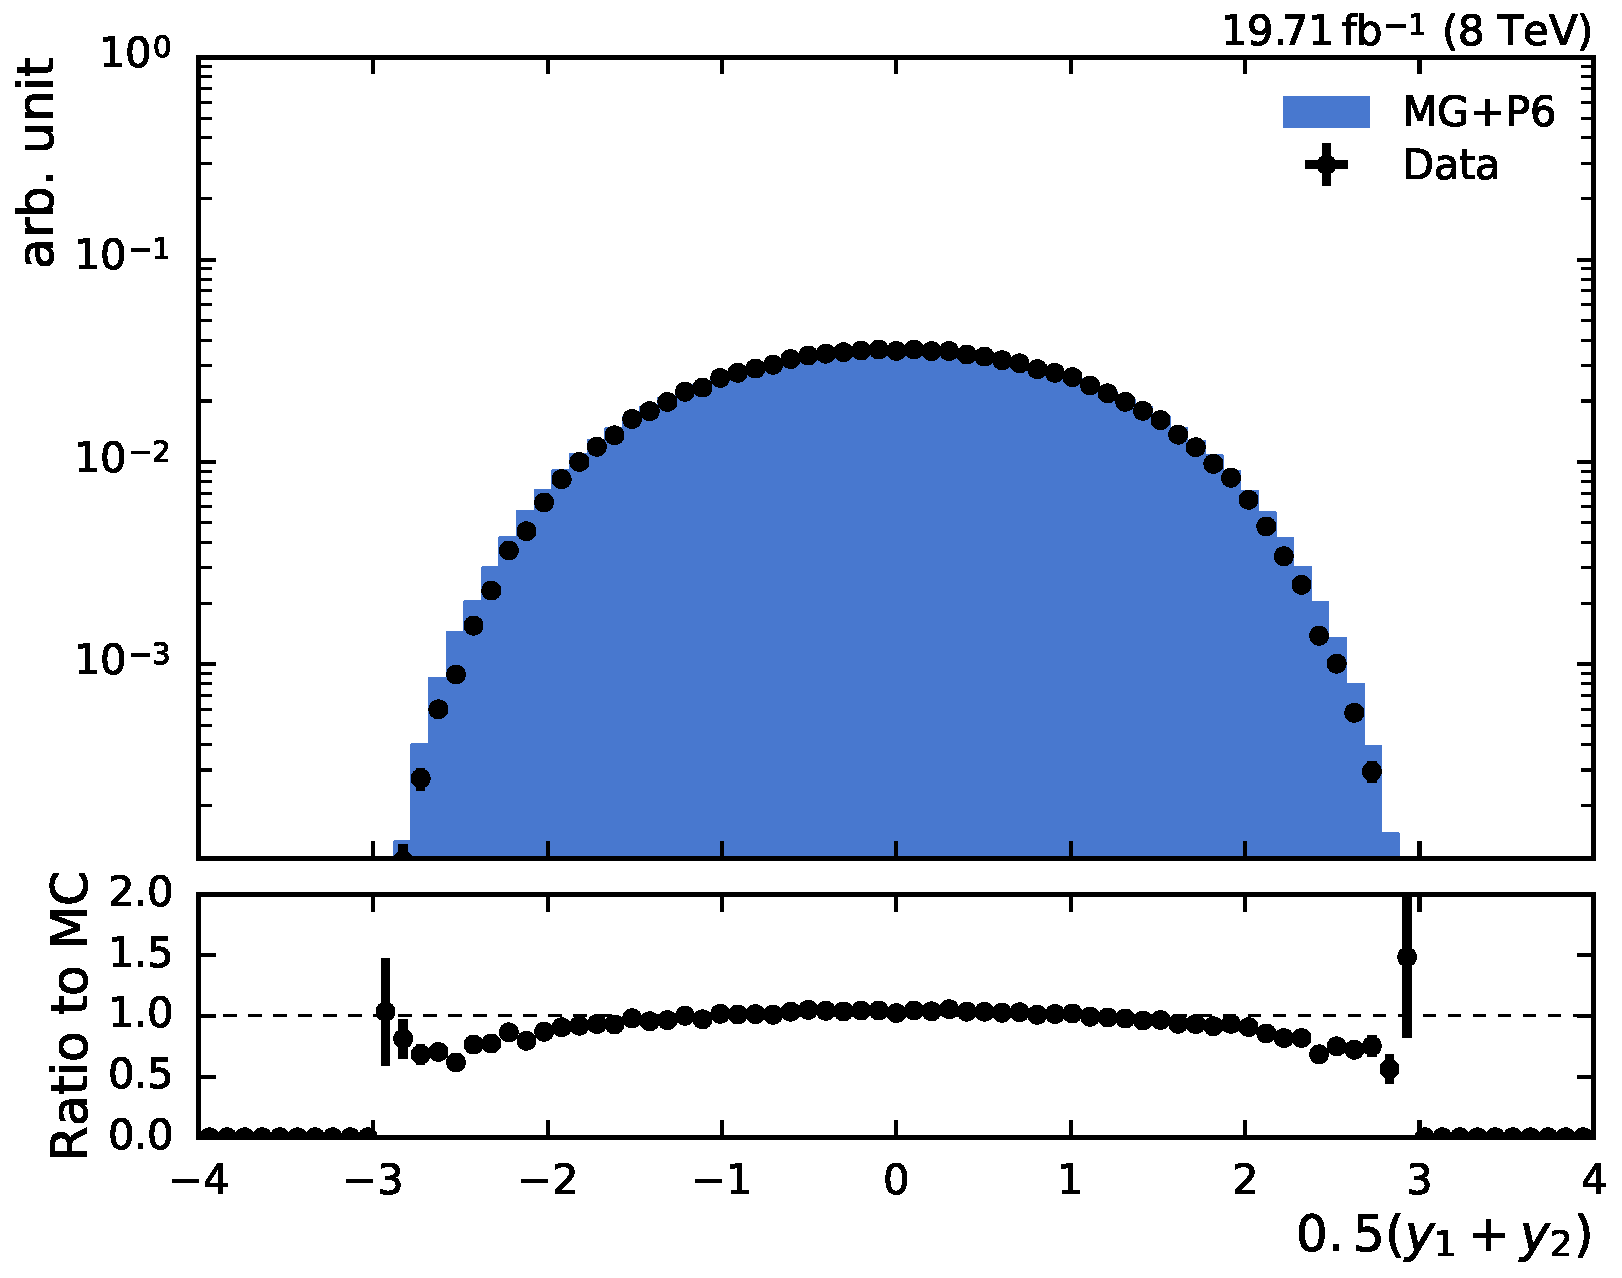
\includegraphics[width=0.47\textwidth]{figures/measurement/dijet_quantities_dijet_yboost.pdf}\hfill
    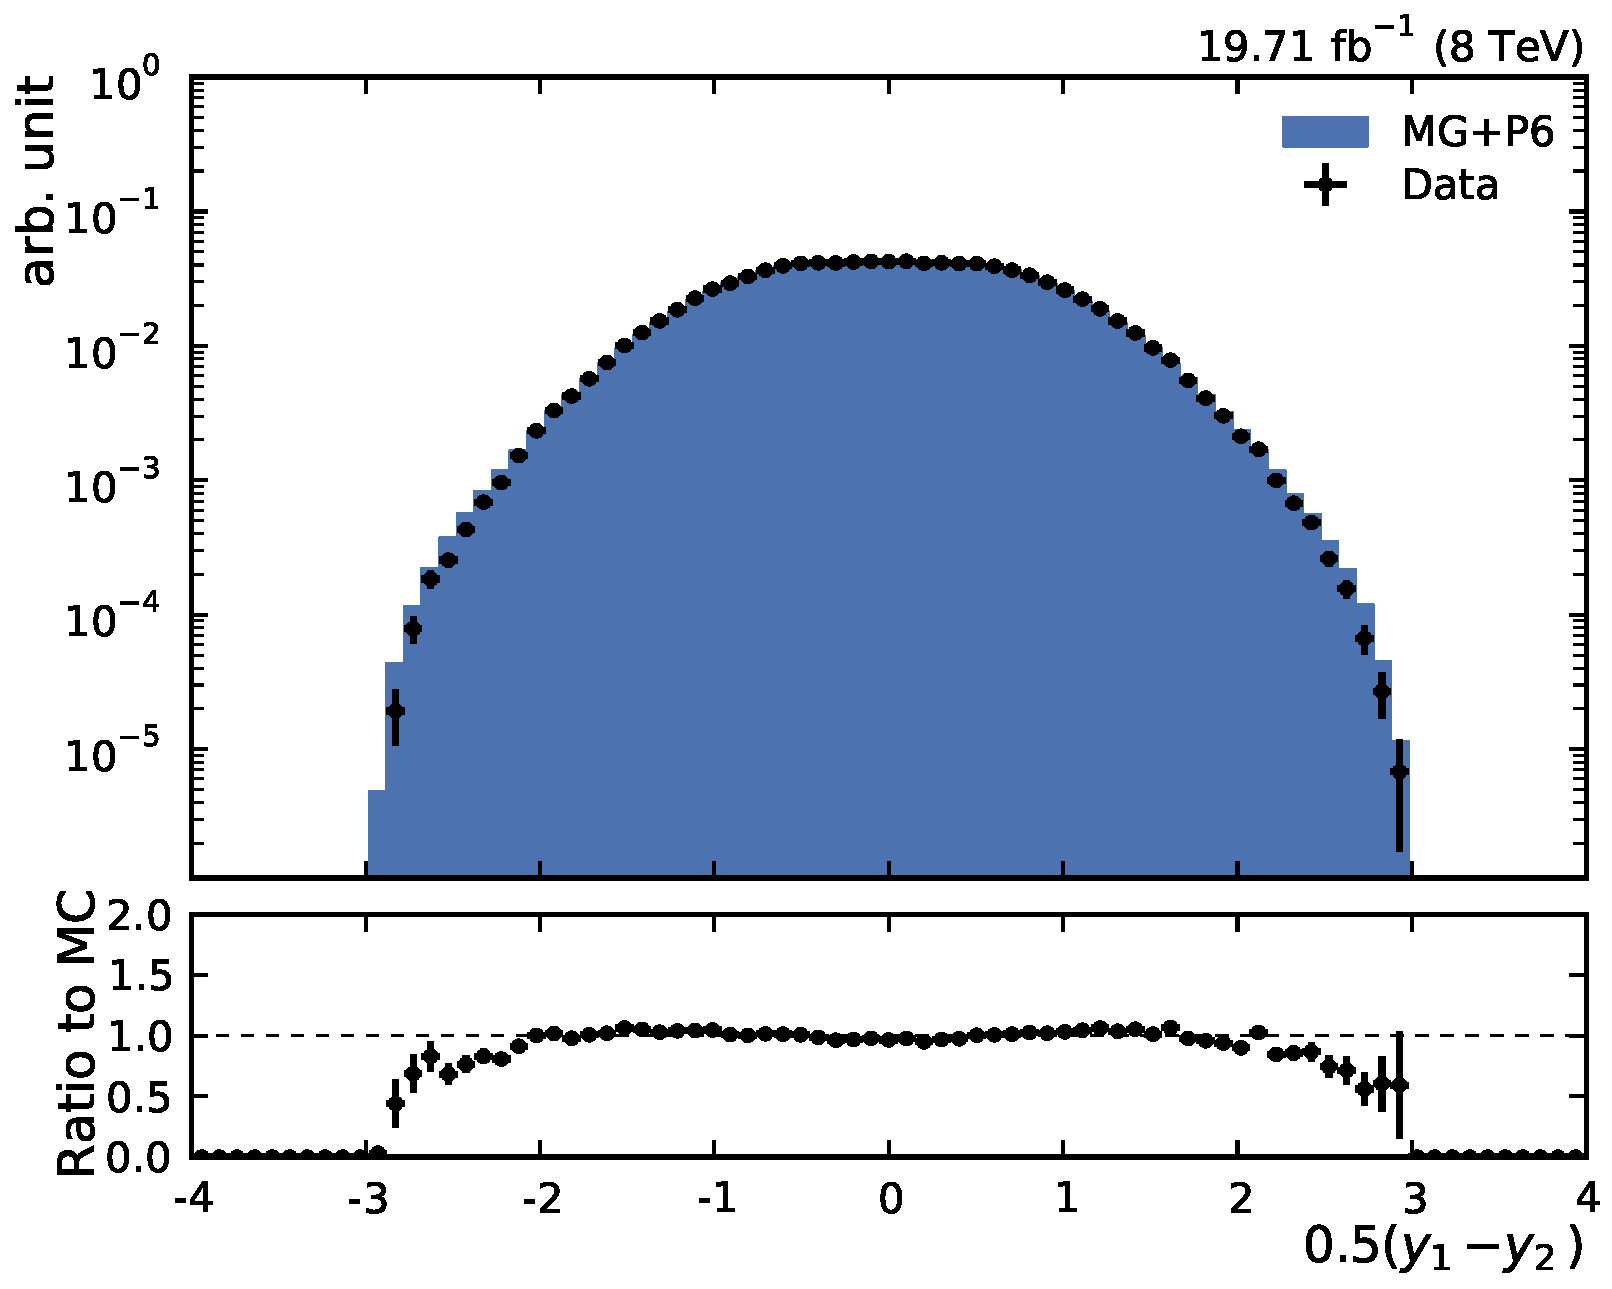
\includegraphics[width=0.47\textwidth]{figures/measurement/dijet_quantities_dijet_ystar.pdf}
    \caption[Kinematic quantities of the dijet system]{Kinematic quantities of
    the dijet system are shown for data (markers) and simulated events
    (histogram). The
    azimuthal separation $\Delta\phi_{1,2}$ and the distance in the $\phi$-$\eta$ plane
    $\Delta R_{1,2}$ are shown in the top row. The dijet mass $M_{1,2}$ and the average
    transverse momentum of the dijet system $\ptavg$ is shown in the middle row. The
    rapidity separation $0.5(y_1 - y_2)$ and the boost $0.5(y_1+y_2)$ is shown in
    the bottom row.}
    \label{fig:controlplots:dijets}
\end{figure}

To illustrate the phase space origin of the dijet events in the various \ystar
and \yboost bins, Fig.~\ref{fig:controlplots:rapidity} shows the event yield as
a function of the leading jet and second jet rapidities. The plot nicely
illustrates, that all SS dijet events are contained in the bins with
large values of \yboost while all OS dijet events are collected in the bins with
larger values of \ystar.

\begin{figure}[htbp]
    \centering
    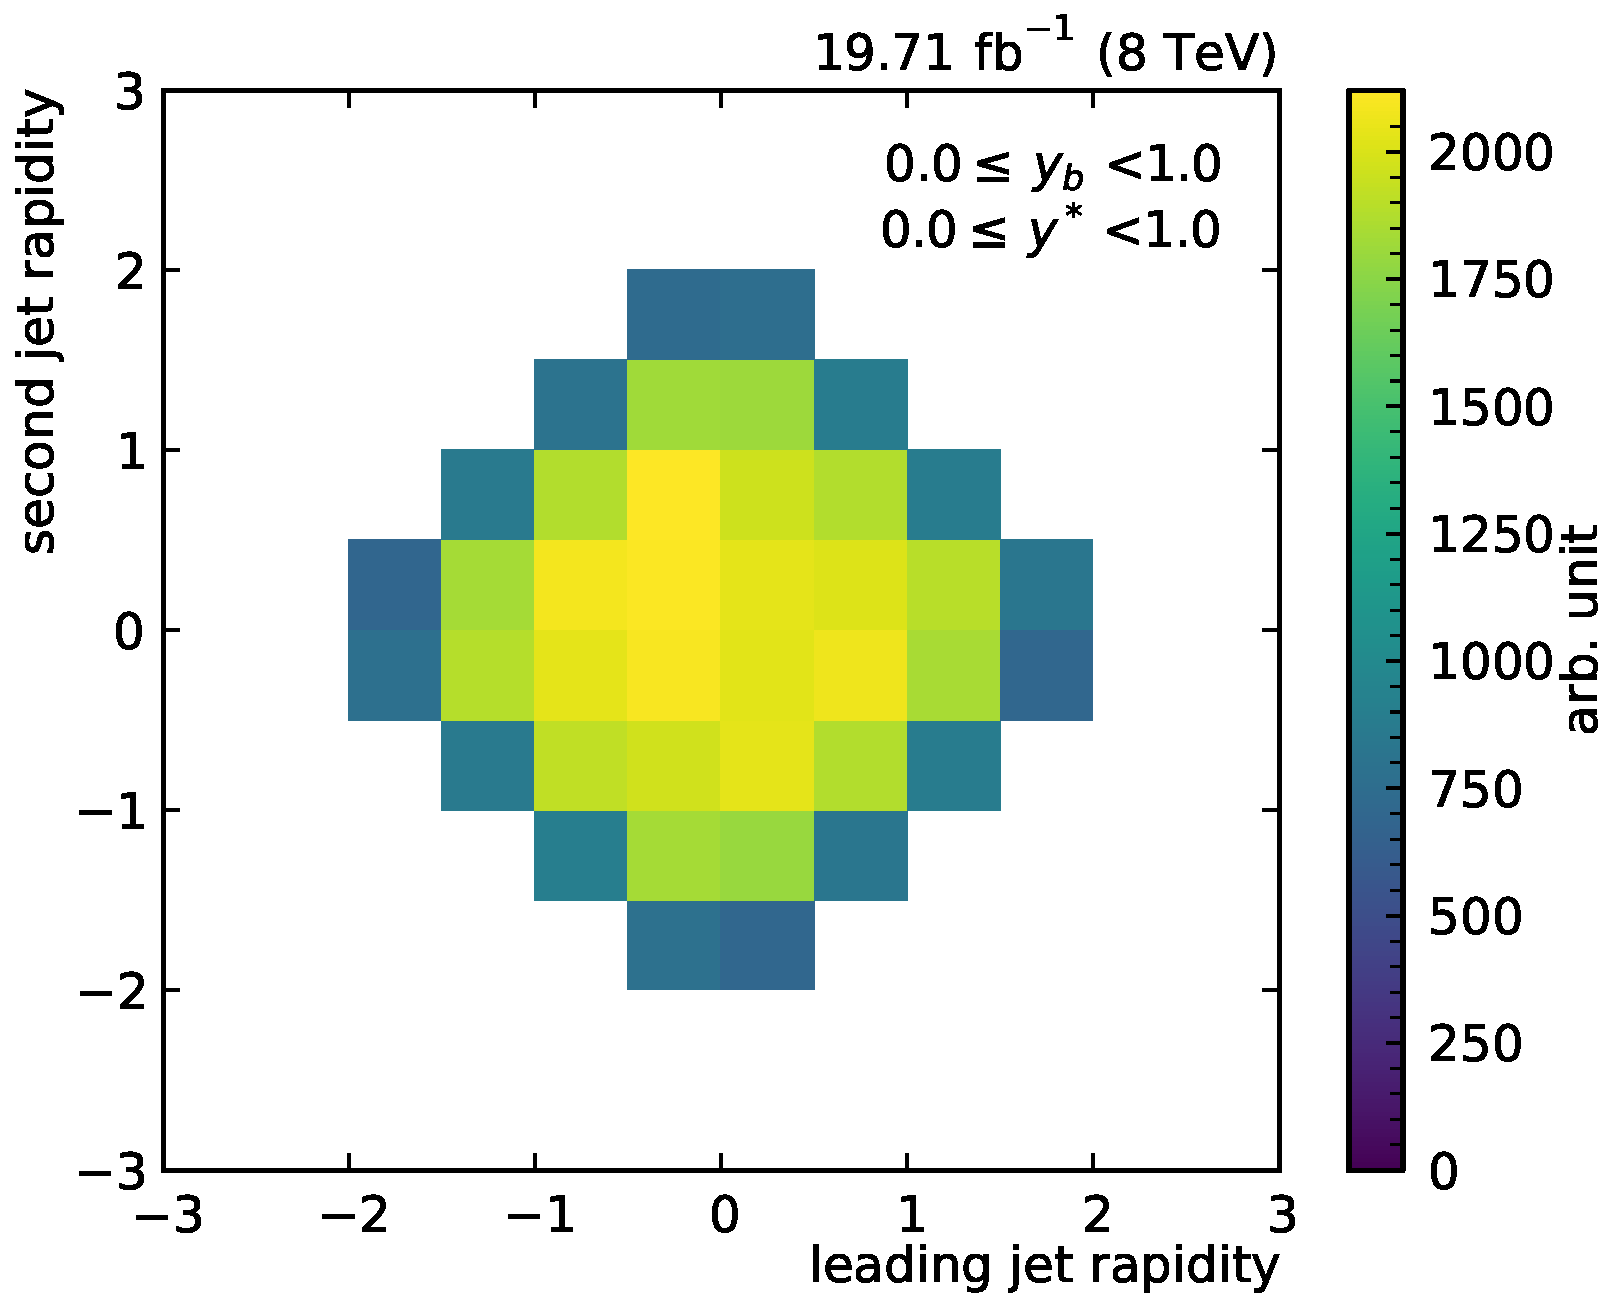
\includegraphics[width=0.47\textwidth]{figures/measurement/jet12_rapidity_yb0ys0.pdf}\hfill
    \includegraphics[width=0.47\textwidth]{figures/measurement/jet12_rapidity_yb0ys1.pdf}
    \includegraphics[width=0.47\textwidth]{figures/measurement/jet12_rapidity_yb0ys2.pdf}\hfill
    \includegraphics[width=0.47\textwidth]{figures/measurement/jet12_rapidity_yb1ys0.pdf}
    \includegraphics[width=0.47\textwidth]{figures/measurement/jet12_rapidity_yb1ys1.pdf}\hfill
    \includegraphics[width=0.47\textwidth]{figures/measurement/jet12_rapidity_yb2ys0.pdf}
    \caption[Rapidities of the two leading jets in the various \ystar and \yboost bins]{
             The distribution of the dijet events in the various \ystar and
             \yboost bins is shown as a function of leading jet and subleading jet
             rapidities. The distributions illustrate the separation of the
             dijet phase space in the various \ystar and \yboost bins.}
    \label{fig:controlplots:rapidity}
\end{figure}


\subsection{Cross Section Comparison}

The Monte Carlo simulation is used to compare the predictions including the
detector simulation to the measured data distribution which is smeared by the
finite detector resolution. Fig.~\ref{fig:ratio_recotodata} shows the prediction
of the Madgraph and the Pythia 8 simulations as a ratio to the measured data
spectrum. While the agreement in the inner detector region is fine, the shape
and especially the normalization of the MC prediction cannot describe the data.
Additionally, a fixed-order prediction of NLOJET++ is shown.  This prediction on
parton level is not corrected for non-perturbative effects. Still it describes
the data, apart from the known non-perturbative and detector resolution effects,
most accurately.

\begin{figure}[htbp]
    \centering
    \includegraphics[width=0.47\textwidth]{figures/measurement/ratio_reco_to_data_yb0ys0.pdf}\hfill
    \includegraphics[width=0.47\textwidth]{figures/measurement/ratio_reco_to_data_yb0ys1.pdf}
    \includegraphics[width=0.47\textwidth]{figures/measurement/ratio_reco_to_data_yb0ys2.pdf}\hfill
    \includegraphics[width=0.47\textwidth]{figures/measurement/ratio_reco_to_data_yb1ys0.pdf}
    \includegraphics[width=0.47\textwidth]{figures/measurement/ratio_reco_to_data_yb1ys1.pdf}\hfill
    \includegraphics[width=0.47\textwidth]{figures/measurement/ratio_reco_to_data_yb2ys0.pdf}
    \caption[Comparison of data with simulated events]{Comparison of the cross
        sections of data and simulated events of LO Monte Carlo generators at
        reconstructed level. The data distributions are normalized to the
        integrated luminosity, the simulated events to the number of generated
        events and the cross section. The ratio of the simulated events to the data
        points is shown.}
    \label{fig:ratio_recotodata}
\end{figure}


\section{Dijet Transverse Momentum  Resolution}
\label{sec:resolution}

The transverse momentum of jets, which are measured in the CMS detector, is
smeared because of the finite detector resolution. In order to correct the
measured cross section for these detector effects, the momentum resolution of
the observable has to be determined. As the simulated events are propagated
through the detector simulation, the information at both particle level and
reconstructed level is available. To compare particle-level jets and
reconstructed jets, the jets belonging together have to be matched to each
other. The distance $\Delta R$ in the $\eta$-$\phi$ plane between two jets is
calculated as
%
\begin{equation}
\Delta R = \sqrt{\Delta \eta^2 + \Delta \phi^2}
\end{equation}
%
and needs to satisfy $\Delta R < 0.3$, roughly half of the jet size parameter
$0.7$. The jets closest to each other in the $\eta$-$\phi$ space are then matched.
However, studies of the \textsc{JERC} working group~\cite{jetmet:resolution}
revealed that the resolution determined in simulated events is better than the
resolution measured in data using data-based techniques. Therefore, the jet
transverse momentum in simulated events is additionally smeared in order to
match the resolution in data.  Table~\ref{tab:res_smearing} gives the smearing
factor together with the assigned uncertainty indicated by the upwards and
downwards variation. To consider the dependence on the detector geometry, the
smearing factor is derived for various $|\eta|$-regions.

\begin{table}[htbp]
\setlength\tabcolsep{4.5pt} 
    \centering
    \caption[Jet energy resolution scale factors]{
             The jet energy resolution in data is significantly worse than in
             simulated events. Therefore, the reconstructed jet transverse
             momentum in simulated events is smeared using a factor $c$ to
             effectively match the resolution in data, following the
             recommendations of the \JetMET group of CMS~\cite{jetmet:resolution}.
             The uncertainty on the resolution is given by an upwards and
             downwards variation $c_\mathrm{up}$ and
             $c_\mathrm{down}$ of the smearing factor $c$.}
    \label{tab:res_smearing}

    \begin{tabular}{lccccccr}
    \toprule
                        &                & \multicolumn{6}{c}{$\bm{|\eta|}$}\\\cmidrule{2-8}
                        & $0.0$ -- $0.5$ & $0.5$ -- $1.1$                                    & $1.1$ -- $1.7$   & $1.7$ --
               $2.3$    & $2.3$ -- $2.8$ & $2.8$ -- $3.2$                                    & $3.2$ -- $5.0$\\
               $\bm{c}$ &                &                                                   &                  &          &       &       & \\\cmidrule{1-1}
    nominal             & 1.079          & 1.099                                             & 1.121            & 1.208    & 1.254 & 1.395 & 1.056\\
    downward            & 1.053          & 1.071                                             & 1.092            & 1.162    & 1.192 & 1.332 & 0.865\\
    upward              & 1.105          & 1.127                                             & 1.150            & 1.254    & 1.316 & 1.458 & 1.247\\
    \bottomrule
    \end{tabular}
\end{table}

The smearing of the reconstructed jet \pt is performed as a multiplicative scale
factor based on the difference of \ptreco and \ptgen, so that \ptreco is shifted
to

\begin{equation}
\ptreco = \max \left( 0, \ptgen + c(\eta) \cdot (\ptreco - \ptgen) \right)
\end{equation}
%
After the smearing, the response which is defined as
%
\begin{equation}
    R = \frac{\ptavg^{\text{reco}}}{\ptavg^{\text{gen}}}
\end{equation}
%
is calculated. Fig.~\ref{fig:gen_vs_reco_over_gen} shows the response as a
function of \ptavggen for each bin. As expected, the relative resolution of low-\pt jets is
significantly worse than the one of high-\pt jets. Since the response is dependent
on both the detector region and the transverse momentum of the jets, the resolution
is calculated as a function of \ptavggen separately in all \ystar and \yboost
bin. 

\begin{figure}[htbp]
    \centering
    \includegraphics[width=0.47\textwidth]{figures/measurement/gen_vs_reco_vs_gen_ptavg_yb0ys0.pdf}\hfill
    \includegraphics[width=0.47\textwidth]{figures/measurement/gen_vs_reco_vs_gen_ptavg_yb0ys1.pdf}
    \includegraphics[width=0.47\textwidth]{figures/measurement/gen_vs_reco_vs_gen_ptavg_yb0ys2.pdf}\hfill
    \includegraphics[width=0.47\textwidth]{figures/measurement/gen_vs_reco_vs_gen_ptavg_yb1ys0.pdf}
    \includegraphics[width=0.47\textwidth]{figures/measurement/gen_vs_reco_vs_gen_ptavg_yb1ys1.pdf}\hfill
    \includegraphics[width=0.47\textwidth]{figures/measurement/gen_vs_reco_vs_gen_ptavg_yb2ys0.pdf}
    \caption[Comparison of particle-level and reconstructed dijet transverse momentum]
            {The response of reconstructed and particle-level jet transverse
                momentum as a function of the particle-level transverse momentum.
                The width of the distribution in each \ptavg bin indicates the
                jet energy resolution, which improves from lower to higher values of \ptavg. The
                resolution is extracted separately for each bin and
                fitted using the NSC-formula.}
    \label{fig:gen_vs_reco_over_gen}
\end{figure}

The resolution is then determined as the width of the distribution in each
\ptavggen
bin, as can be seen in Fig.~\ref{fig:resolution_bin}. Both a Gaussian function
as well as a double-sided Crystal Ball function have been studied in order to
describe the observed behavior. Despite the large differences in the
description of the non-Gaussian tails emphasized by the logarithmic
representation, the width obtained from the fit of the distribution is very similar.
Nonetheless, the Crystal Ball function is used to determine the resolution
$\Delta \ptavggen / \ptavggen$ as
it better describes the measured distributions, especially in the low-\pt
region where the non-Gaussian tails are more pronounced.

\begin{figure}[h!tbp]
    \centering
    \includegraphics[width=0.47\textwidth]{figures/measurement/resolution_yb0ys0_bin10.pdf}\hfill
    \includegraphics[width=0.47\textwidth]{figures/measurement/resolution_yb0ys0_bin10_cb.pdf}
    \caption[Gaussian and Crystal Ball fit of resolution.]{The resolution in
        each \ptavg bin is fitted using a Gaussian (left) or a double-sided Crystal Ball
        function (right). The fit using the Crystal Ball function better describes the
        non-Gaussian tails of the distribution. Therefore, it is favored in the
    determination of the jet energy resolution.}
    \label{fig:resolution_bin}
\end{figure}

Fig.~\ref{fig:resolution_ptavg} shows the resolution in each \ystar and
\yboost bin as a function of \ptavg. The relative resolution is fitted using a
modified version of the NSC formula.
%
\begin{equation}
    \frac{\Delta_{\ptavggen}}{\ptavggen} (\ptavggen) = \sqrt{\sgn{N}
    \left(\frac{N}{\ptavggen}\right)^2 +
    \left(\frac{\ptavggen}{\text{GeV}}\right)^s \frac{S^2}{\ptavggen} + C^2 }
    \label{eq:resolution}
\end{equation}
%
The formula is based on the calorimetric NSC formula which describes the resolution
with terms for noise $N$, a stochastic component $S$ and a constant
shift $C$. Especially in the low-\pt region, in which the tracking has a
non-negligible influence on the resolution due to the PF algorithm, a
slightly better fit is obtained by using the modified resolution given in
Formula~\ref{eq:resolution}. However, the influence of the different resolution formulas
on the unfolded cross section is negligible as the spectrum starts at
much higher \ptavg. Table~\ref{tab:resolution_parameters} gives the parameters of
the fit in each \ystar and \yboost bin of the measurement.


\begin{figure}[htbp]
    \centering
    \includegraphics[width=0.8\textwidth]{figures/measurement/resolution_ptavg_crystalball.pdf}
    \caption[Relative momentum resolution vs \ptavg]{The jet energy resolution as a
        function of \ptavggen is shown for all \ystar and \yboost bins. The data points
        indicate the separate determinations while the solid lines give the
    results of the fits using the NSC-formula.}
    \label{fig:resolution_ptavg}
\end{figure}


\begin{table}[htbp]
    \centering
    \caption[Relative dijet transverse momentum resolution parameters]
    {Fitted parameters of the modified NSC formula characterizing the transverse
    momentum resolution in the \ystar and \yboost bins.}
    \label{tab:resolution_parameters}
    \begin{tabular}{cccccc}
        \toprule
         \yboost & \ystar & N      & S     & C      & s\\\midrule
         0 -- 1  & 0 -- 1 & -2.68  & 1.43  & 0.03   & -0.26\\
         0 -- 1  & 1 -- 2 & -8.00  & 5.81  & 0.04   & -0.73\\
         0 -- 1  & 2 -- 3 & -0.02  & 1.98  & -0.018 & -0.36\\
         1 -- 2  & 0 -- 1 & -8.13  & 5.96  & 0.04   & -0.73\\
         1 -- 2  & 1 -- 2 &  2.85  & 1.16  & 0.02   & -0.17\\
         2 -- 3  & 0 -- 1 &  3.96  & 1.23  & 0.00   & -0.18\\\hline
            \bottomrule
    \end{tabular}
\end{table}

\section{Unfolding of the Measurement}
\label{sec:unfolding}

The final goal of this analysis is the comparison of the triple-differential
dijet cross section measurement with higher-order QCD calculations on
particle level. Due to finite detector acceptance and resolution, the jet
transverse momentum is smeared causing differences between the particle-level
\ptavggen spectrum and the measured spectrum \ptavgreco. To allow particle level comparisons,
the measurement has to be unfolded. Thus, calculations from future Monte Carlo
event generators can easily be compared with this measurement without the need to
apply a detector simulation.

In this analysis, the iterative d'Agostini algorithm~\cite{DAgostini:1994zf} is
used, which is implemented in the RooUnfold~\cite{Adye:2011gm} package. The
unfolding process is regularized by the number of iteration steps in this
algorithm. A higher number of iterations yields a reduced \chisq but also
increases the uncertainty and introduces larger bin-by-bin fluctuations and
correlations. The regularization is optimized using simulated events and best
results with low bin-by-bin correlations and low \chisq are achieved using
four iterations in the unfolding algorithm.

In principal, the response matrix for the unfolding algorithm can be populated
directly using simulated events as they contain both the particle-level and
reconstructed jets. However, this method has several drawbacks. The LO
prediction does not describe the shape of the distribution in some phase space
regions. Moreover, the
limited number of events in the Monte Carlo sample, especially at high
rapidities and high transverse momenta, introduces non-negligible statistical
fluctuations in the response matrix. Because of these undesirable effects, an
alternative strategy is employed to populate the response matrix.

Relying on the good description of the data spectrum by NLO predictions, a forward
smearing technique is applied. The NLO prediction, obtained with the CT14-NLO PDF
set and corrected for non-perturbative effects, is fitted using the function

\begin{equation}
    f(\ptavg) = A_0 \left(
    \frac{\ptavg}{A_3}\right)^{-A_1}\left(1-\frac{\ptavg}{A_3}\right)^{A_2},
\end{equation}

which describes both the normalization and shape of the distribution. Using toy
Monte Carlo events, a flat \ptavg spectrum weighted according to the fitted NLO
distribution is generated. This distribution resembles the fastNLO cross section
prediction and is used as the particle-level \ptavg spectrum. All generated
events are then smeared using the resolution function obtained in
Sec.~\ref{sec:resolution}. The generation of these Monte Carlo toy events is
very fast, and the response matrices can be filled with more than 100 million
events each, resulting in negligible statistical fluctuations.
Fig.~\ref{fig:res_matrix} shows the response matrices used in the unfolding
process. The matrices in the figure are normalized to the number of events in
each particle-level bin to improve the readability. They are diagonal with small
off-diagonal elements, which represent migrations between neighboring \ptavg
bins.

\begin{figure}[htp]
    \centering
    \includegraphics[width=0.47\textwidth]{figures/measurement/res_matrix_ptavg_normalized_yb0ys0.pdf}\hfill
    \includegraphics[width=0.47\textwidth]{figures/measurement/res_matrix_ptavg_normalized_yb0ys1.pdf}
    \includegraphics[width=0.47\textwidth]{figures/measurement/res_matrix_ptavg_normalized_yb0ys2.pdf}\hfill
    \includegraphics[width=0.47\textwidth]{figures/measurement/res_matrix_ptavg_normalized_yb1ys0.pdf}
    \includegraphics[width=0.47\textwidth]{figures/measurement/res_matrix_ptavg_normalized_yb1ys1.pdf}\hfill
    \includegraphics[width=0.47\textwidth]{figures/measurement/res_matrix_ptavg_normalized_yb2ys0.pdf}
    \caption[Response matrix used for the unfolding]{Response matrices
        illustrating the bin migrations. They are obtained using the forward smearing method and are normalized
        to the number of events of particle-level events to improve readability. The response
        matrices are diagonal with small off-diagonal entries indicating bin
    migrations between neighboring \ptavg bins.}
    \label{fig:res_matrix}
\end{figure}

A closure test was performed by unfolding the generated smeared spectrum in two
ways. Once, the smeared spectrum was obtained using the same events which were
used to fill the response matrix and once, the spectrum was generated using
statistically independent events. In the first case, exactly the same truth
spectrum should be re-obtained after unfolding, while in the second case, the
results should agree within statistical uncertainties.
Fig.~\ref{fig:unf_closure_test} demonstrates that both assumptions hold for the
applied unfolding technique.

\begin{figure}[htp]
    \centering
    \includegraphics[width=0.47\textwidth]{figures/measurement/unf_nlo_check_yb0ys0.pdf}\hfill
    \includegraphics[width=0.47\textwidth]{figures/measurement/unf_nlo_check_yb0ys1.pdf}
    \includegraphics[width=0.47\textwidth]{figures/measurement/unf_nlo_check_yb0ys2.pdf}\hfill
    \includegraphics[width=0.47\textwidth]{figures/measurement/unf_nlo_check_yb1ys0.pdf}
    \includegraphics[width=0.47\textwidth]{figures/measurement/unf_nlo_check_yb1ys1.pdf}\hfill
    \includegraphics[width=0.47\textwidth]{figures/measurement/unf_nlo_check_yb2ys0.pdf}
    \caption[Closure check of unfolding technique]{Closure test of the employed unfolding
    procedure. Once, the smeared spectrum is obtained from the same events that
were used to fill the response matrix and once from statistically independent
events. As expected, unfolding the former spectrum (green line) again yields exactly the
truth spectrum. Unfolding the statistically independently smeared spectrum
gives compatible results within statistical uncertainties (blue line).}
    \label{fig:unf_closure_test}
\end{figure}

Another closure test was performed by filling the response matrices directly
from the simulated events of the Madgraph data sample and comparing the unfolded
cross section with the one obtained using the forward smearing technique. In
both cases, the results are consistent within uncertainties. However, the
statistical uncertainties are very large due to the limited number of events in
the Madgraph sample.

The applied unfolding technique does not consider fluctuations between
\ystar and \yboost bins. However, migrations between neighboring \ystar and
\yboost bins were studied and found to be very small. Therefore, it is justified
to perform the unfolding in each \ystar and \yboost bin separately.

Statistical uncertainties of the data distributions are propagated through the
unfolding procedure using toy experiments. The procedure as well as its results
are discussed in detail in Sec.~\ref{sec:stat_unf_uncert} when experimental
sources of uncertainties are discussed. The unfolded cross sections are shown in
Sec.~\ref{sec:nlo_comparisons}, in which the comparison to NLO calculations is
presented.

\section{Experimental Uncertainties}
\label{sec:experimental_uncertainties}

In this section all experimental uncertainties which affect the cross
section measurement are discussed: The statistical uncertainties, jet energy
scale and resolution uncertainties, the luminosity uncertainty, and
a residual uncertainty accounting for systematic errors due to the jet ID and
trigger efficiencies. 

An overview depicting all experimental uncertainties can be found in
Fig.~\ref{fig:exp_unc_overview} at the end of the section. It presents all
sources of experimental uncertainty in combination with the total experimental
uncertainty, obtained by adding all individual sources in quadrature. The total
uncertainty amounts to \SI{4}{\percent} in the measurement bins involving jets at central
rapidity and increases up to \SI{25}{\percent} in bins where jets from worse understood
phase space regions contribute, see Table~\ref{tab:data:expunc}.

\begin{table}[htbp]
    \centering
    \caption[Summary of experimental uncertainties]
       {Five experimental sources of uncertainty affect the accuracy of the
        measurement. The dominant source arises from jet energy scale
        corrections. The total uncertainties are as small as 5\% in the best understood
        region and increase up to 25\% in worst understood phase space regions.}
    \label{tab:data:expunc}
    \begin{tabular}{cccc}
    \toprule
    \textbf{Uncertainty source} & \textbf{Min}       & \textbf{Average}   & \textbf{Max}\\\midrule
    Jet energy scale            & \SI{2.5}{\percent} & \SI{4.0}{\percent} & \SI{11}{\percent}\\
    Luminosity                  & \SI{2.6}{\percent} & \SI{2.6}{\percent} & \SI{2.6}{\percent}\\
    Jet energy resolution       & \SI{0.3}{\percent} & \SI{1}{\percent} & \SI{2.5}{\percent}\\
    Statistical                 & \SI{0.1}{\percent} & \SI{1.5}{\percent} & \SI{22}{\percent}\\
    Residual                    & \SI{1}{\percent} & \SI{1}{\percent} & \SI{1}{\percent}\\\midrule
    \textbf{Total}              & \SI{4}{\percent} & \SI{6}{\percent} & \SI{25}{\percent}\\
    \bottomrule
    \end{tabular}
\end{table}

\subsection {Uncertainty on Luminosity Measurement}
\label{sec:luminosity_uncertainty}

As discussed in Sec.~\ref{sec:lumi_measurement}, the luminosity is measured from
the number of clusters in the silicon pixel detector. The uncertainty on the
luminosity measurement for the 2012 LHC run is estimated to be 2.5\% (syst.) and
0.5\% (stat.)~\cite{CMS-PAS-LUM-13-001}. As the luminosity uncertainty
translates into a normalization uncertainty on any absolute cross section
measurement, a combined systematic uncertainty of 2.6\% is assigned, which is
fully correlated across all bins.

\subsection{Unfolding and Statistical Uncertainties}
\label{sec:stat_unf_uncert}

Statistical uncertainties of data points are propagated through the unfolding
using a toy MC technique in which the data are smeared according to
their statistical uncertainties. Then, the unfolding procedure is repeated using
the smeared spectrum. One million of such toy spectra are used to
propagate the statistical uncertainty. Fig.~\ref{fig:statunc_relative} shows
the relative statistical uncertainty before and after the unfolding procedure.
The uncertainty slightly increases during the unfolding process.

\begin{figure}[htbp]
    \centering
    \includegraphics[width=0.47\textwidth]{figures/measurement/statunc_fractional_yb0ys0.pdf}\hfill
    \includegraphics[width=0.47\textwidth]{figures/measurement/statunc_fractional_yb0ys1.pdf}
    \includegraphics[width=0.47\textwidth]{figures/measurement/statunc_fractional_yb0ys2.pdf}\hfill
    \includegraphics[width=0.47\textwidth]{figures/measurement/statunc_fractional_yb1ys0.pdf}
    \includegraphics[width=0.47\textwidth]{figures/measurement/statunc_fractional_yb1ys1.pdf}\hfill
    \includegraphics[width=0.47\textwidth]{figures/measurement/statunc_fractional_yb2ys0.pdf}
    \caption[Statistical uncertainty of measured and unfolded spectrum]{The
    statistical uncertainties of the measured and the unfolded data. Depending
    on the unfolding procedure, the uncertainties can slightly increase.}
    \label{fig:statunc_relative}
\end{figure}

Furthermore, the unfolding introduces a correlation between bins due to event
migrations. These correlations are significant for neighboring bins in \pt and
negligible between bins far apart in the phase space.
Fig.~\ref{fig:corr_unfolding_nlo} shows the correlations of the statistical
uncertainty after the unfolding. Of course, these correlations have to be taken
into account in any statistical analysis of the data such as a PDF fit.

\begin{figure}[htbp]
    \centering
    \includegraphics[width=0.47\textwidth]{figures/measurement/unf_nlo_corr_yb0ys0.pdf}\hfill
    \includegraphics[width=0.47\textwidth]{figures/measurement/unf_nlo_corr_yb0ys1.pdf}
    \includegraphics[width=0.47\textwidth]{figures/measurement/unf_nlo_corr_yb0ys2.pdf}\hfill
    \includegraphics[width=0.47\textwidth]{figures/measurement/unf_nlo_corr_yb1ys0.pdf}
    \includegraphics[width=0.47\textwidth]{figures/measurement/unf_nlo_corr_yb1ys1.pdf}\hfill
    \includegraphics[width=0.47\textwidth]{figures/measurement/unf_nlo_corr_yb2ys0.pdf}
    \caption[Correlations of statistical uncertainty]{Correlations of the
        statistical uncertainty introduced by the unfolding procedure.
        Neighboring bins exhibit a significant correlation or anti-correlation
        through bin migrations.}
    \label{fig:corr_unfolding_nlo}
\end{figure}

\subsection{Jet Energy Correction Uncertainties}

The dominant part of the experimental uncertainties derives from the jet energy
calibration, which corrects the measured jet energy for a variety of detector
effects and is discussed in Sec.~\ref{sec:jec}. As the corrections are afflicted
with multiple sources of systematic uncertainty, all sources are propagated
individually to the cross section to preserve their correlations.

The JEC uncertainties are split into 25 mutually independent sources of
uncertainty, in which each source is fully correlated in \pt and $\eta$,
but uncorrelated to all other sources, and presents a $1\sigma$
shift. As these uncertainties can be asymmetric, the upwards and downwards
variation of each source are treated separately. The sum in quadrature of all
sources yields the total JEC uncertainty. Therefore, they can be treated
in exactly the same way as the PDF eigenvector sets, which were discussed in
Sec.~\ref{sec:pdf_uncertainties}. The sources of uncertainty are grouped in four
categories according to their origin. In the following, a short summary of the
sources is given. More details about the jet energy corrections and
uncertainties are given in~\cite{jec_8tev}. The
Figs.~\ref{fig:jec_relunc_0}--\ref{fig:jec_relunc_5} in the appendix show the
size of each of the 25 sources separately.

\begin{description}
    \item[Pileup JES] Differences in the transverse momentum between the true
        offset and the random cone offset are observed in simulated events. This
        difference is propagated using Z/$\gamma$+jet and dijet balancing
        methods to estimate the residual pileup uncertainty after the
        calibration.
    \item[Relative JES] The relative $\eta$-dependent corrections calibrate
        forward jets using balanced dijet events. The largest contribution to
        the uncertainty arises from jet energy resolution and soft radiation
        bias corrections. 
    \item[Absolute JES]  The absolute calibration of the jet energy scale relies
        on Z/$\gamma$+jet and multi-jet events. The uncertainties are related to
        the lepton momentum scale for muon and the single pion response in the
        HCAL. Observed differences in applied methods can be traced back to neutrinos
        and ISR and are accounted for in these sources of uncertainty.
    \item[Flavor JES] Differences in the flavor response are studied using
        simulation by cross-checking the results with quark- and gluon-tagged
        $\gamma$+jet and Z+jet events. The uncertainty is derived based on
        differences observed in the Pythia 6 and Herwig++ simulation.
\end{description}

\subsection{Jet Energy Resolution Uncertainty}

The jet energy resolution, which was derived in Sec.~\ref{sec:resolution}, is
used to populate the response matrix using a forward smearing technique in the
unfolding procedure. Therefore, a dependence of the
unfolded cross section on the jet energy resolution is introduced. 

Table~\ref{tab:res_smearing} shows the smearing factors, which were applied on
reconstructed simulated events to obtain the actual resolution in data. The
official recommendations include offset variations of these smearing factors to
estimate the uncertainty on the resolution and are also given in
Table~\ref{tab:res_smearing}. The determination of the resolution is repeated
with the applied upwards and downwards variation of the resolution smearing
factor. The unfolding procedure is also reiterated using the variations of the
resolution, and the differences of the obtained cross section to the nominal
cross section are accounted for with a systematic uncertainty. The influence on
the cross section is comparably small, about 1\% in low \ystar and \yboost and
increasing up to 3\% for the highest \ystar value.

An overview of all uncertainties is given in Fig.~\ref{fig:exp_unc_overview},
which shows their relative size in each bin.

\begin{figure}[htbp]
    \centering
    \includegraphics[width=0.46\textwidth]{figures/measurement/exp_unc_overview_yb0ys0.pdf}\hfill
    \includegraphics[width=0.46\textwidth]{figures/measurement/exp_unc_overview_yb0ys1.pdf}
    \includegraphics[width=0.46\textwidth]{figures/measurement/exp_unc_overview_yb0ys2.pdf}\hfill
    \includegraphics[width=0.46\textwidth]{figures/measurement/exp_unc_overview_yb1ys0.pdf}
    \includegraphics[width=0.46\textwidth]{figures/measurement/exp_unc_overview_yb1ys1.pdf}\hfill
    \includegraphics[width=0.46\textwidth]{figures/measurement/exp_unc_overview_yb2ys0.pdf}
    \caption[Overview of experimental uncertainties]{Overview of all
    experimental uncertainties affecting the cross section measurement. The
    error bars indicate the statistical uncertainty after unfolding. The colored
    lines give the uncertainties resulting from jet energy corrections, jet energy
    resolution, luminosity and residual effects. The total uncertainty is yielded by
    adding the individual sources of uncertainty in quadrature.}
    \label{fig:exp_unc_overview}
\end{figure}

\section{Comparison with NLO Predictions}
\label{sec:nlo_comparisons}

After unfolding the measurement, it is finally possible to
compare the measured cross sections with the NLO calculations obtained in
Sec.~\ref{sec:theory_predictions}. A general comparison is given in
Fig.~\ref{fig:measurement_result}, which shows the data overlaid with the
\NLOJETPP prediction obtained with the NNPDF 3.0 PDF set. The fixed order NLO
calculation is corrected for non-perturbative effects. The measurement
and the NLO predictions agree over many orders of magnitude of the cross section.

\begin{figure}[h!tbp]
    \centering
    \includegraphics[width=0.9\textwidth]{figures/measurement/ptavg_spectrum.pdf}\hfill
    \caption[Spectrum of the triple-differential dijet cross section]{The
    triple-differential dijet cross section in six bins of \ystar and \yboost. The
    data are indicated by different markers for each bin and the theory obtained
    with \NLOJETPP and NNPDF 3.0 is depicted by colored lines. Apart from the
    boosted region, the data is well described by NLO theory calculations over many orders of magnitude.}
    \label{fig:measurement_result}
\end{figure}

A more detailed comparison is possible when the ratio of data to theory is
calculated. Fig~\ref{fig:ratio_nnpdf30_mccomp_nlo} presents
such ratios for calculations using different PDF sets. Apart
from a few phase space regions, the predictions using all PDF sets, except for
the ABM 11 PDF set well describe the data. The predictions using the ABM 11 PDF
set systematically underestimate the data. This behavior is well known, \eg
from~\cite{Khachatryan:2014waa,Stober:2012abc}, and can be traced back to a
soft gluon PDF accompanied with a low value of \asmz in the PDF.

In the central region, at low \yboost and \ystar, a systematic difference of up
to \SI{20}{\percent} between data and NLO predictions is observed for transverse
momenta beyond \SI{1}{\TeV}. This mismatch is presumably caused by missing electroweak
corrections, which are positive and sizable at low rapidity and \pt larger
than \SI{1}{\TeV}~\cite{Dittmaier:2012kx,Khachatryan:2014waa}. Theory colleagues are currently working on providing the
electroweak corrections specifically for this measurement, but the corrections
were not available in time.
\todo{Change if EWK available}

Figure~\ref{fig:ratio_nnpdf30_nlo} shows ratios of the data to the predictions of
the \NLOJETPP, Powheg, and Herwig 7 NLO MC generators. There are significant differences
observed between the predictions of the studied MC generators. These could originate
from the PDFs or the scale choices in each MC generator which are
not trivially adaptable. In general, Herwig 7 better describes the data in the
central region while Powheg prevails in the forward region.

Especially phase space regions in which the data discriminate between the
predictions of different PDF sets are interesting for PDF studies. As
discussed in Sec.~\ref{sec:crosssection_definition}, the bins involving boosted
dijet events, in which the accessed fractional proton momenta $x_1$ and $x_2$
are very different, are predestined for PDF studies. The predictions of the
different PDF sets, especially compared to the ones of the NNPDF set, yield
different results in the boosted region and are afflicted with large PDF
uncertainties. Moreover, none of the investigated PDF sets yields a good
description of the data in this phase space region, see
Fig.~\ref{fig:ratio_nnpdf30_nlo} bottom right, making it a very interesting
subject for PDF studies.

\section{Summary}

In this chapter, the complete data analysis of the triple-differential dijet
cross section measurement has been presented. The reconstructed spectrum has
been unfolded with the iterative d'Agostini algorithm to correct for all
detector dependent effects. By comparing with NLO pQCD calculations, it was
found that the data are well described in most of the studied phase
space. Systematic deviations at some edges of the investigated phase space were
observed and probably could be traced back to missing electroweak corrections and the
PDFs. The high experimental precision of the data and the comprehensive study of
all sources of uncertainties including their correlations allows to include this
measurement in a PDF fit to derive constraints.

\begin{figure}[htbp]
    \centering
    \includegraphics[width=0.48\textwidth]{figures/measurement/ratio_to_NNPDF30+np_totcomp_yb0ys0.pdf}\hfill
    \includegraphics[width=0.48\textwidth]{figures/measurement/ratio_to_NNPDF30+np_totcomp_yb0ys1.pdf}
    \includegraphics[width=0.48\textwidth]{figures/measurement/ratio_to_NNPDF30+np_totcomp_yb0ys2.pdf}\hfill
    \includegraphics[width=0.48\textwidth]{figures/measurement/ratio_to_NNPDF30+np_totcomp_yb1ys0.pdf}
    \includegraphics[width=0.48\textwidth]{figures/measurement/ratio_to_NNPDF30+np_totcomp_yb1ys1.pdf}\hfill
    \includegraphics[width=0.48\textwidth]{figures/measurement/ratio_to_NNPDF30+np_totcomp_yb2ys0.pdf}
    \caption[Ratio of measured cross sections to prediction using different PDFs]{
    Ratio of the triple-differential dijet cross section to the \NLOJETPP
    prediction ($\mu=\ptmax e^{0.3 \ystar}$) using the NNPDF 3.0 set. The data
    points including statistical uncertainties are indicated by markers, the total
    experimental uncertainty is represented by the hatched band. The blue
    band shows the PDF and NP uncertainties quadratically added and the continuous colored lines give the
    predictions calculated with different PDF sets.}
    \label{fig:ratio_nnpdf30_nlo}
\end{figure}

\begin{figure}[htbp]
    \centering
    \includegraphics[width=0.48\textwidth]{figures/measurement/ratio_to_NNPDF30+np_varcomp_yb0ys0.pdf}\hfill
    \includegraphics[width=0.48\textwidth]{figures/measurement/ratio_to_NNPDF30+np_varcomp_yb0ys1.pdf}
    \includegraphics[width=0.48\textwidth]{figures/measurement/ratio_to_NNPDF30+np_varcomp_yb0ys2.pdf}\hfill
    \includegraphics[width=0.48\textwidth]{figures/measurement/ratio_to_NNPDF30+np_varcomp_yb1ys0.pdf}
    \includegraphics[width=0.48\textwidth]{figures/measurement/ratio_to_NNPDF30+np_varcomp_yb1ys1.pdf}\hfill
    \includegraphics[width=0.48\textwidth]{figures/measurement/ratio_to_NNPDF30+np_varcomp_yb2ys0.pdf}
    \caption[Ratio of measured cross sections to predictions using different MC event generators]{
    Ratio of the triple-differential dijet cross sections to the \NLOJETPP
    prediction ($\mu=\ptmax e^{0.3 \ystar}$) using the NNPDF 3.0 set. The data
    points including statistical uncertainties are indicated by markers, the
    total experimental uncertainty is represented by the hatched band. The blue band
    shows the PDF and NP uncertainties quadratically added. The predictions of the NLO MC generators
    Powheg+P8 and Herwig 7 are depicted by the red and green lines, respectively.}
    \label{fig:ratio_nnpdf30_mccomp_nlo}
\end{figure}


